\chapter{Appendices for Chapter~3}

\section{MC generator parameters for the signal models}
\label{appendix:parameters1}
$q* \to W/Z + jet$ in Pythia6 with Tune Z2:
\begin{verbatim}
processParmeters = cms.vsting(
        'MSEL=0 ! (D=1) 0 to select full user control',
        'MSTP(6)=1 ! excited quarks',
        'MSUB(147)=1 ! qg->d*',
        'MSUB(148)=1 ! qg->u*',
        'PMAS(343,1)=${mass} ! mass of d*',
        'PMAS(344,1)=${mass} ! mass of u*',
        'RTCM(41)=${scale} ! Lambda = mass',
        'RTCM(43)=1.0 ! f',
        'RTCM(44)=1.0 ! fp',
        'RTCM(45)=1.0 ! fs',
        '4000001:ALLOFF',
        '4000001:ONIFMATCH 1 23 ! qW=1 23, qZ=2 24',
        '4000002:ALLOFF',
        '4000002:ONIFMATCH 2 23 ! qW=2 23, qZ=1 24',
)
\end{verbatim}

$G_{RS} \to WW/ZZ$ in Pythia6 with Tune Z2:
\begin{verbatim}
processParameters = cms.vstring(
        'PMAS(347,1)=${mass} ! mass of RS Graviton',
        'PARP(50)=${kmpl} ! 0.54 == c=0.1 (k/M_PL=0.1)',
        'MSEL=0 ! (D=1) 0 to select full user control',
        'MSUB(391)=1 ! q qbar -> G*',
        'MSUB(392)=1 ! g g -> G*',
        '5000039:ALLOFF ! Turn off all decays of G*',
        '5000039:ONIFANY 24 ! Turn on the decays WW=24, ZZ=23',
)
\end{verbatim}

$G_{RS} \to WW/ZZ$ in Herwig++:
\begin{verbatim}
   configFiles = cms.vstring('RS.model'),
   parameterSets = cms.vstring(
      'cm7TeV',
      'pdfCTEQ6L1',
      'productionParameters',
      'basicSetup',
      'setParticlesStableForDetector',
   ),
   productionParameters = cms.vstring(
'cd /Herwig/NewPhysics',
'insert ResConstructor:Incoming 0 /Herwig/Particles/g',
'insert ResConstructor:Incoming 1 /Herwig/Particles/u',
'insert ResConstructor:Incoming 2 /Herwig/Particles/ubar',
'insert ResConstructor:Incoming 3 /Herwig/Particles/d',
'insert ResConstructor:Incoming 4 /Herwig/Particles/dbar',
'insert ResConstructor:Intermediates 0 /Herwig/Particles/Graviton',
'insert ResConstructor:Outgoing 0 /Herwig/Particles/W+', #Z0
'set RS/Model:Lambda_pi 10000*GeV',
'set /Herwig/Particles/Graviton:NominalMass ${scale}*GeV',
   )
\end{verbatim}

$W' \to WZ$ in Pythia6 with Tune Z2:
\begin{verbatim}
processParameters = cms.vstring(
        'PMAS(34,1)=\${mass} ! mass of Wprime',
        'MSEL=0 ! (D=1) 0 to select full user control',
        'MSUB(142)=1 ! qq->Wprime',
        'MDME(311,1)=0 ! Wprime->dubar',   
     'MDME(312,1)=0 ! Wprime->dcbar',
        'MDME(313,1)=0 ! Wprime->dtbar',
        'MDME(315,1)=0 ! Wprime->subar',       
	 'MDME(316,1)=0 ! Wprime->scbar',
        'MDME(317,1)=0 ! Wprime->stbar',
        'MDME(319,1)=0 ! Wprime->bubar',      
	  'MDME(320,1)=0 ! Wprime->bcbar',
        'MDME(321,1)=0 ! Wprime->btbar',
        'MDME(327,1)=0 ! Wprime->enu',     
	   'MDME(328,1)=0 ! Wprime->munu',
        'MDME(329,1)=0 ! Wprime->taunu',
        'MDME(331,1)=1 ! Wprime->WZ',
        'MDME(332,1)=0 ! Wprime->Wgamma',
        'MDME(333,1)=0 ! Wprime->Wh0',
)
\end{verbatim}

%\clearpage

%\subsection{Pile up study in signal MC}

%\begin{figure}[htbp]
%\centering
%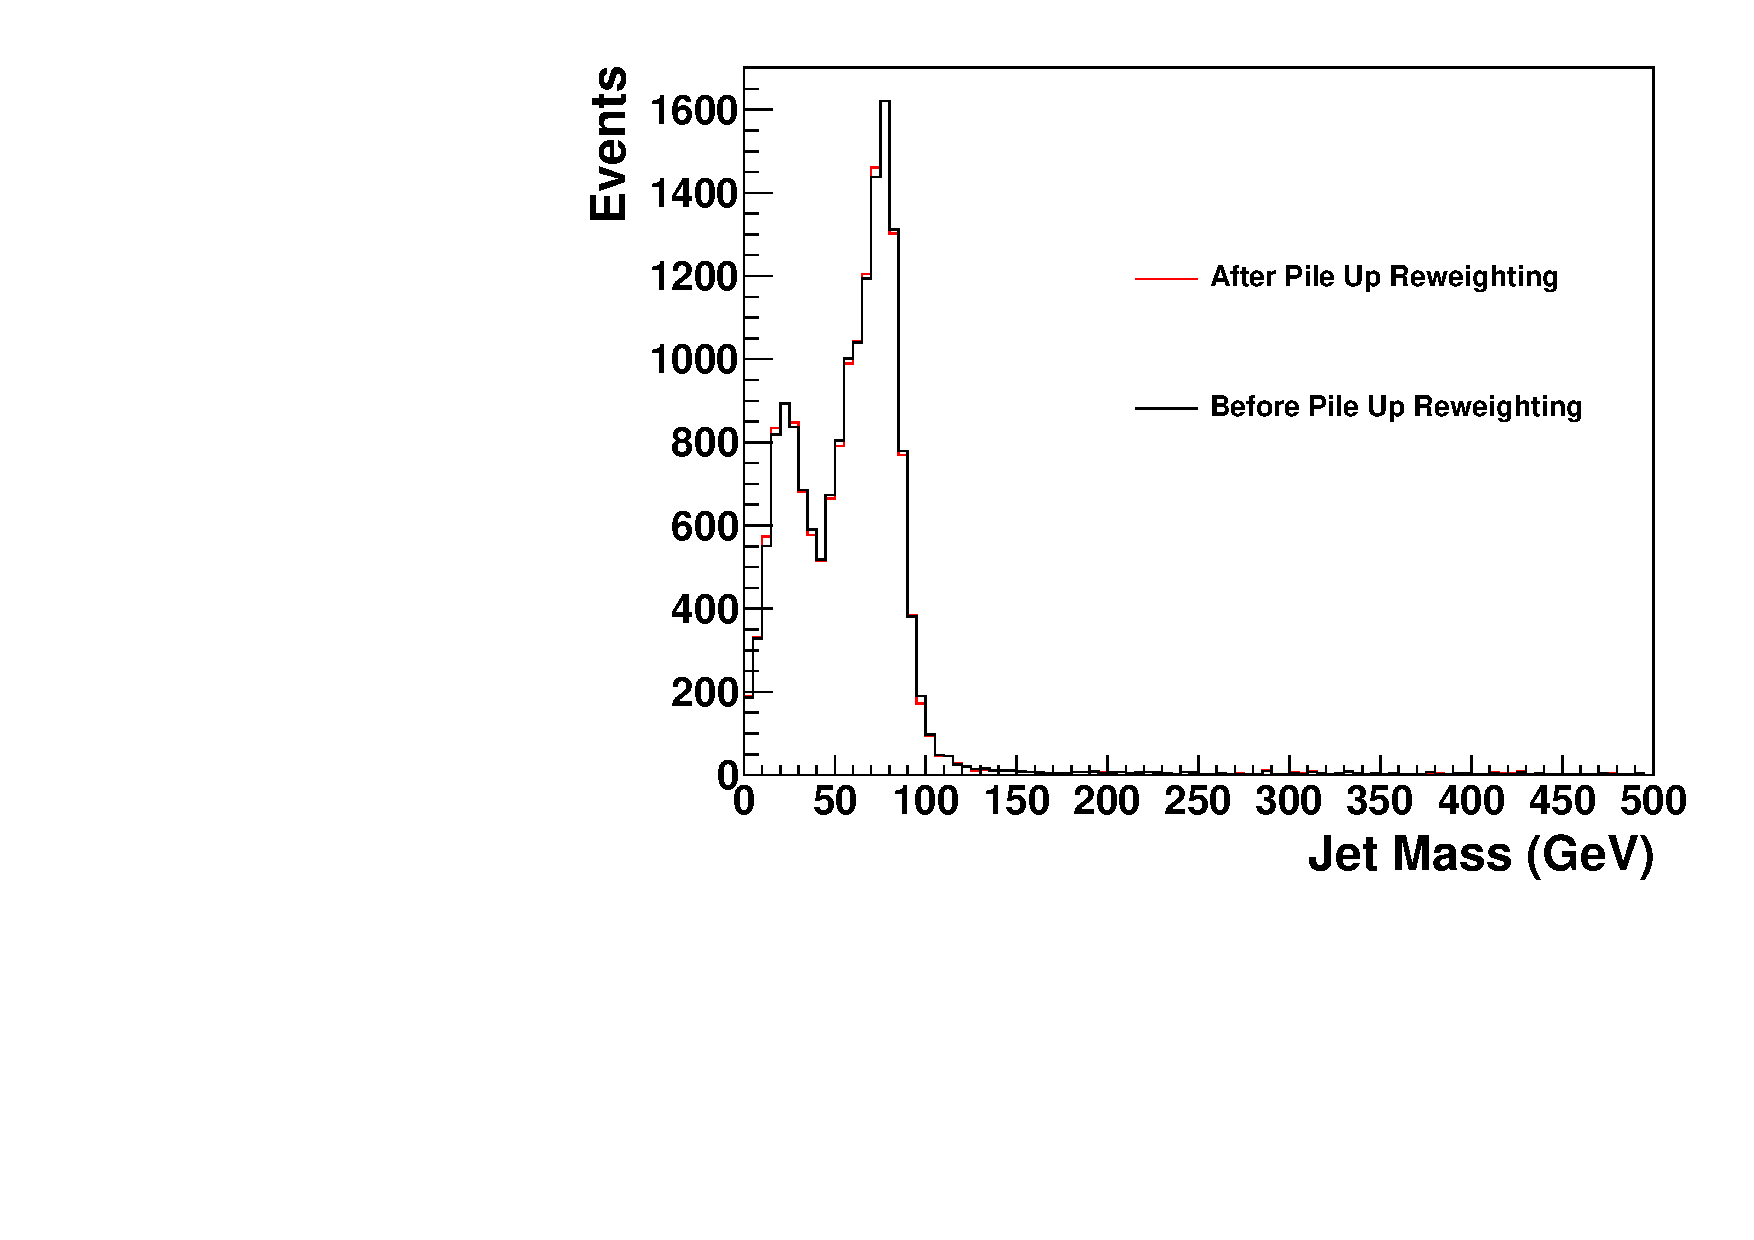
\includegraphics[width=0.48\textwidth]{EXO-12-024/figs/sig-pile-up/jetMassPileUp.pdf}
%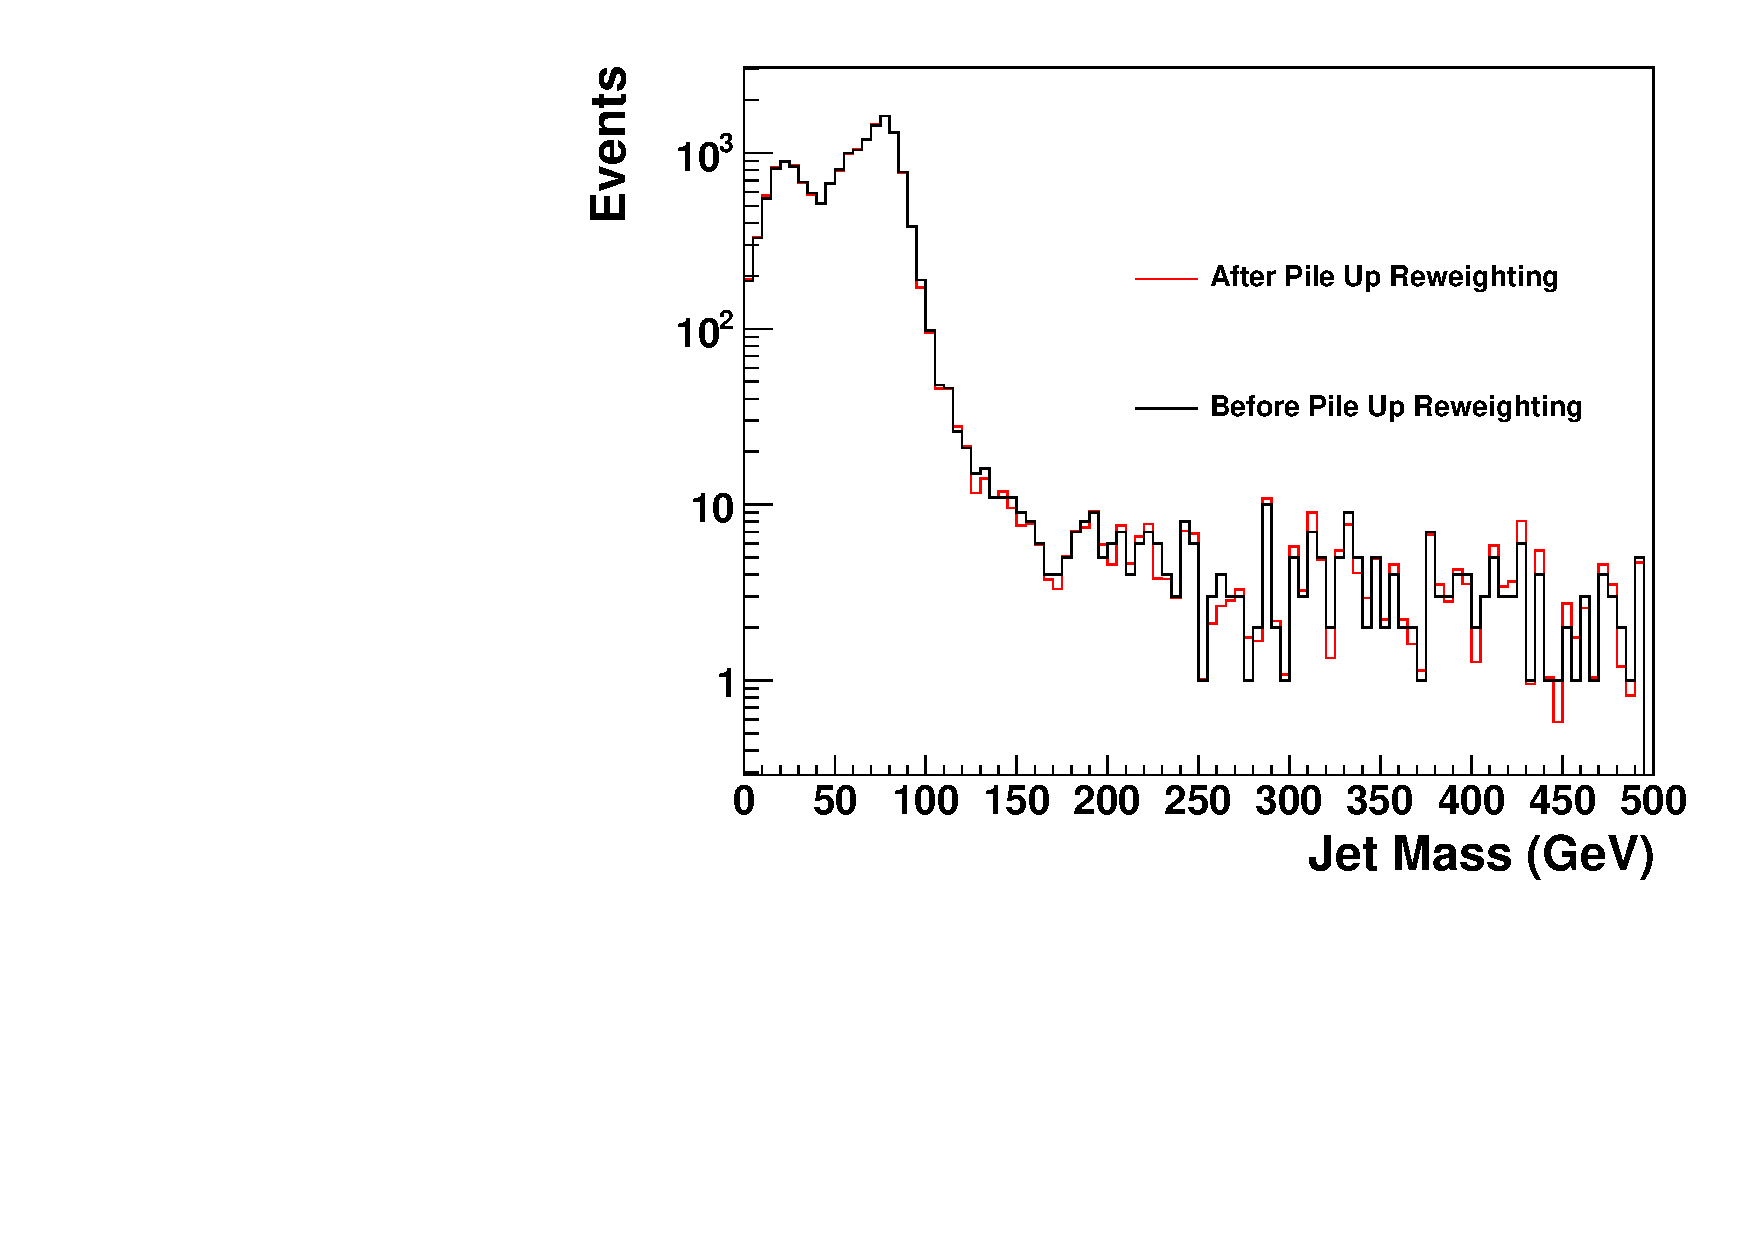
\includegraphics[width=0.48\textwidth]{EXO-12-024/figs/sig-pile-up/jetMassPileUpLog.pdf}
%\caption{Comparsion for jet mass distribution for $G_{RS} \to ZZ (3.0TeV)$. Plot on the right is the corresponding log scale plot.}
%\label{figs:sig-pile-up-jet-mass}
%\end{figure}

%\begin{figure}[htbp]
%\centering
%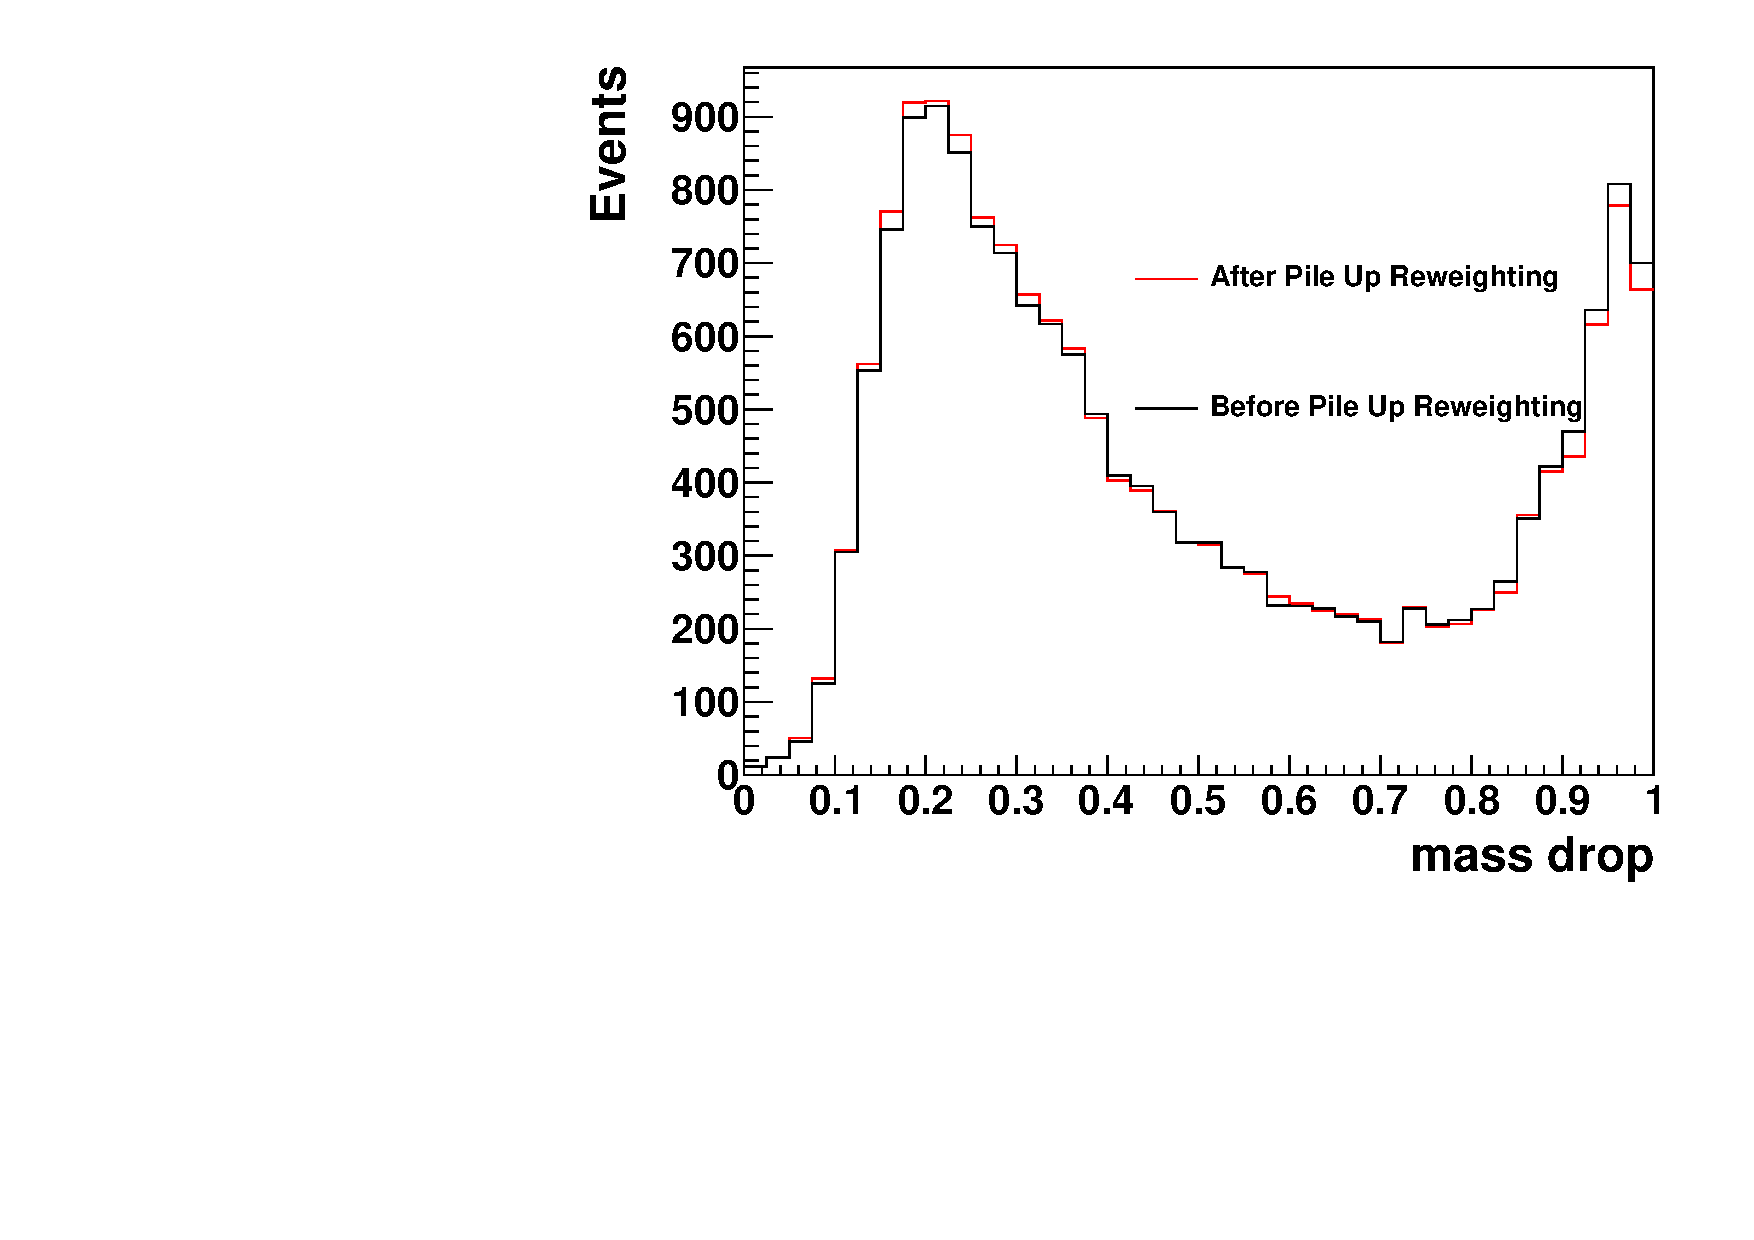
\includegraphics[width=0.48\textwidth]{EXO-12-024/figs/sig-pile-up/massDropPileUp.pdf}
%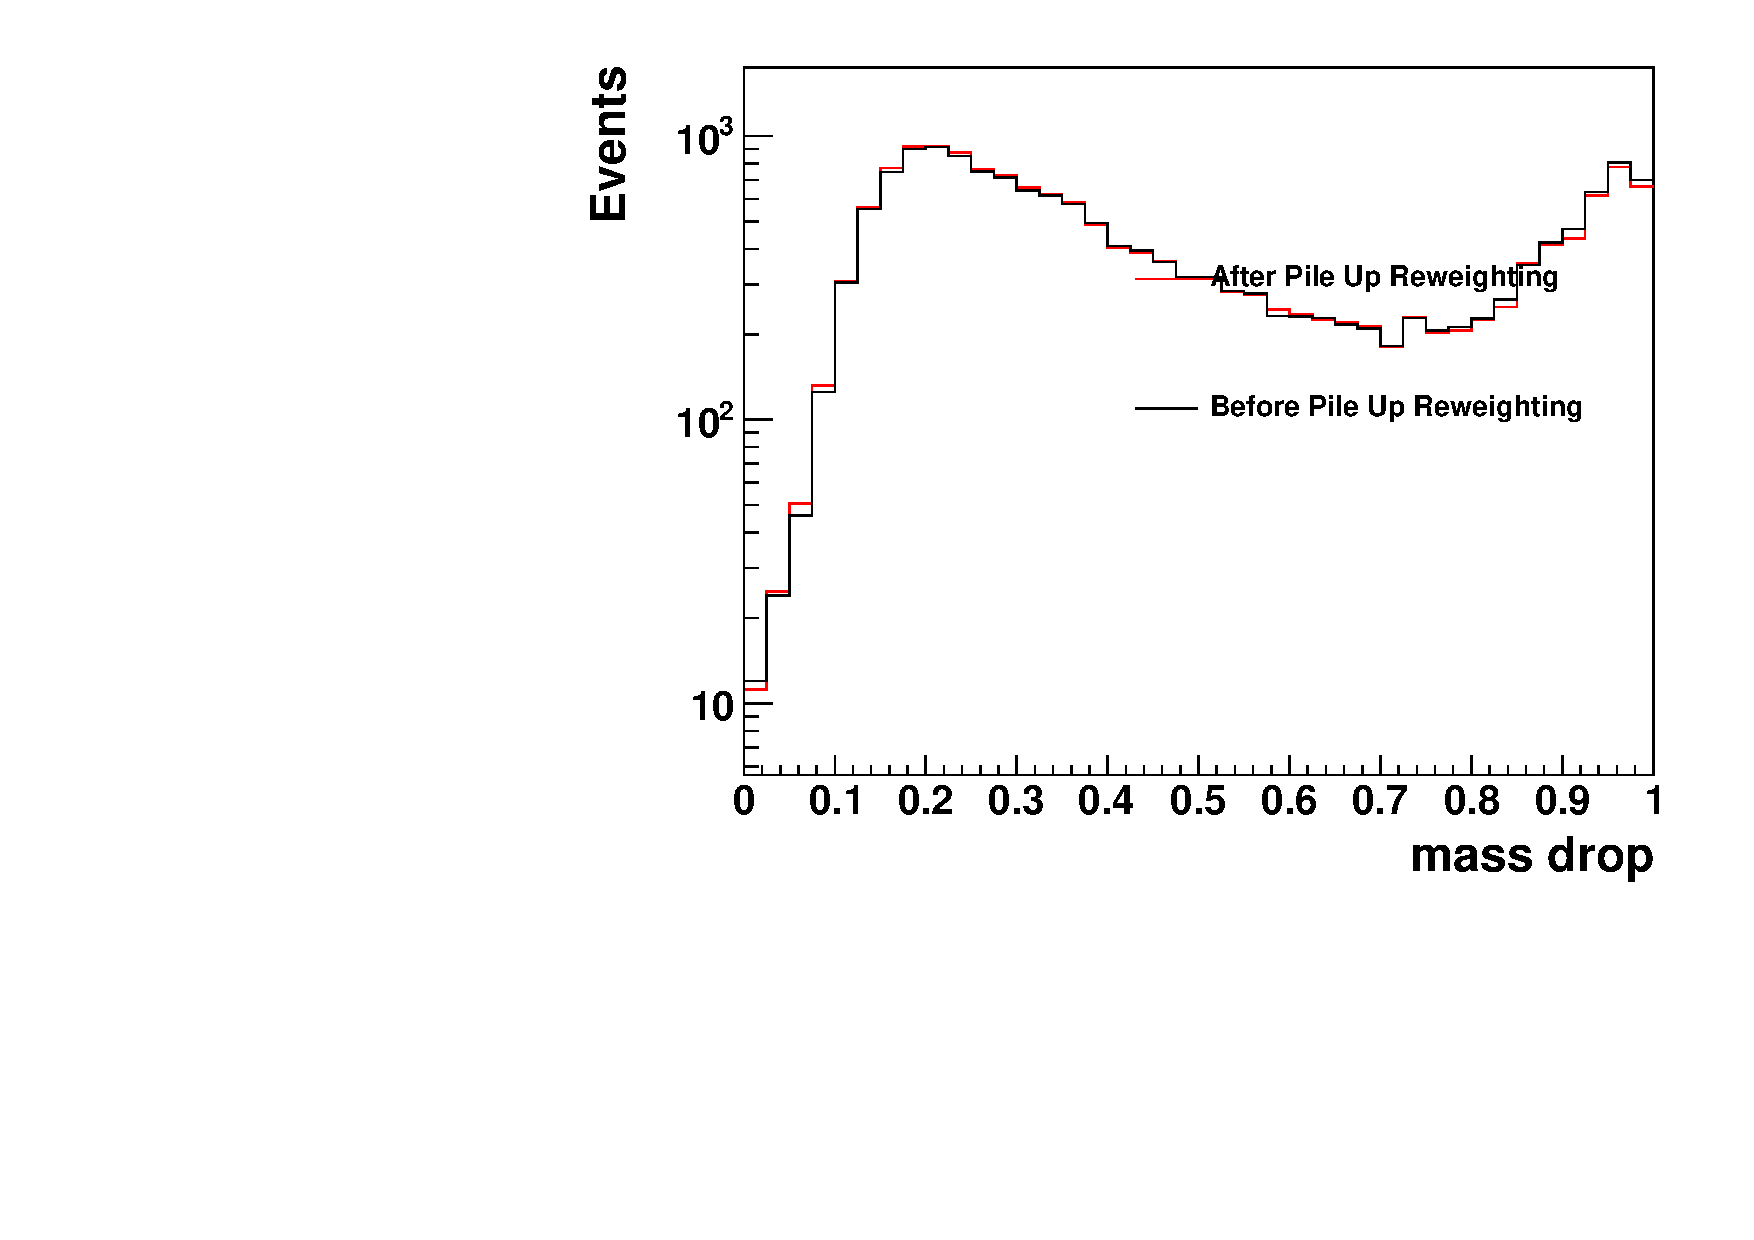
\includegraphics[width=0.48\textwidth]{EXO-12-024/figs/sig-pile-up/massDropPileUpLog.pdf}
%\caption{Comparsion for mass drop distribution for $G_{RS} \to ZZ (3.0TeV)$. Plot on the right is the corresponding log scale plot.}
%\label{figs:sig-pile-up-mass-drop}
%\end{figure}

%\begin{figure}[htbp]
%\centering
%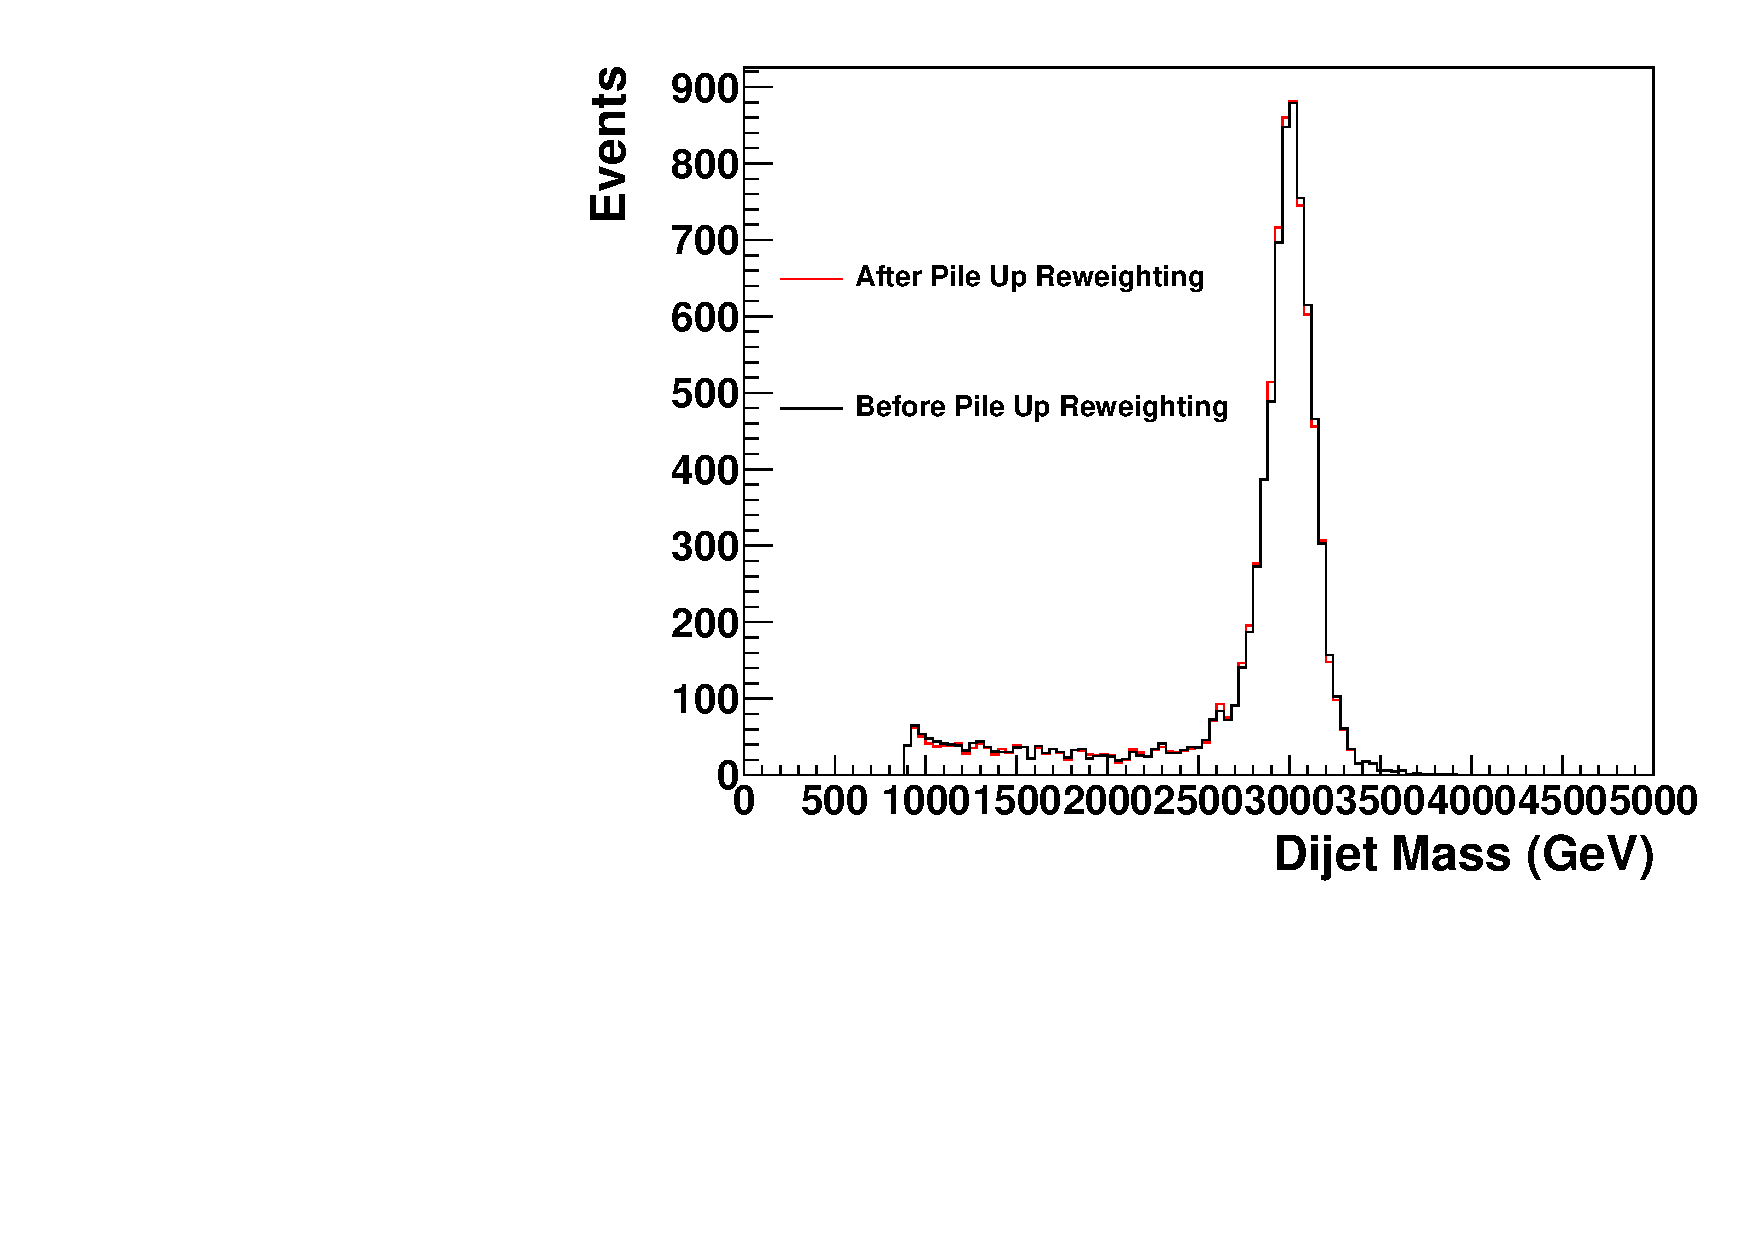
\includegraphics[width=0.88\textwidth]{EXO-12-024/figs/sig-pile-up/DijetMassPileUp.pdf}
%\caption{Comparsion for dijet mass distribution for $G_{RS} \to ZZ (3.0TeV)$. Plot on the right is the corresponding log scale plot.}
%\label{figs:sig-pile-up-dijetmass}
%\end{figure}

\clearpage

\subsection{Signal shape at high resonance mass}

\begin{figure}[!htpb]
\centering
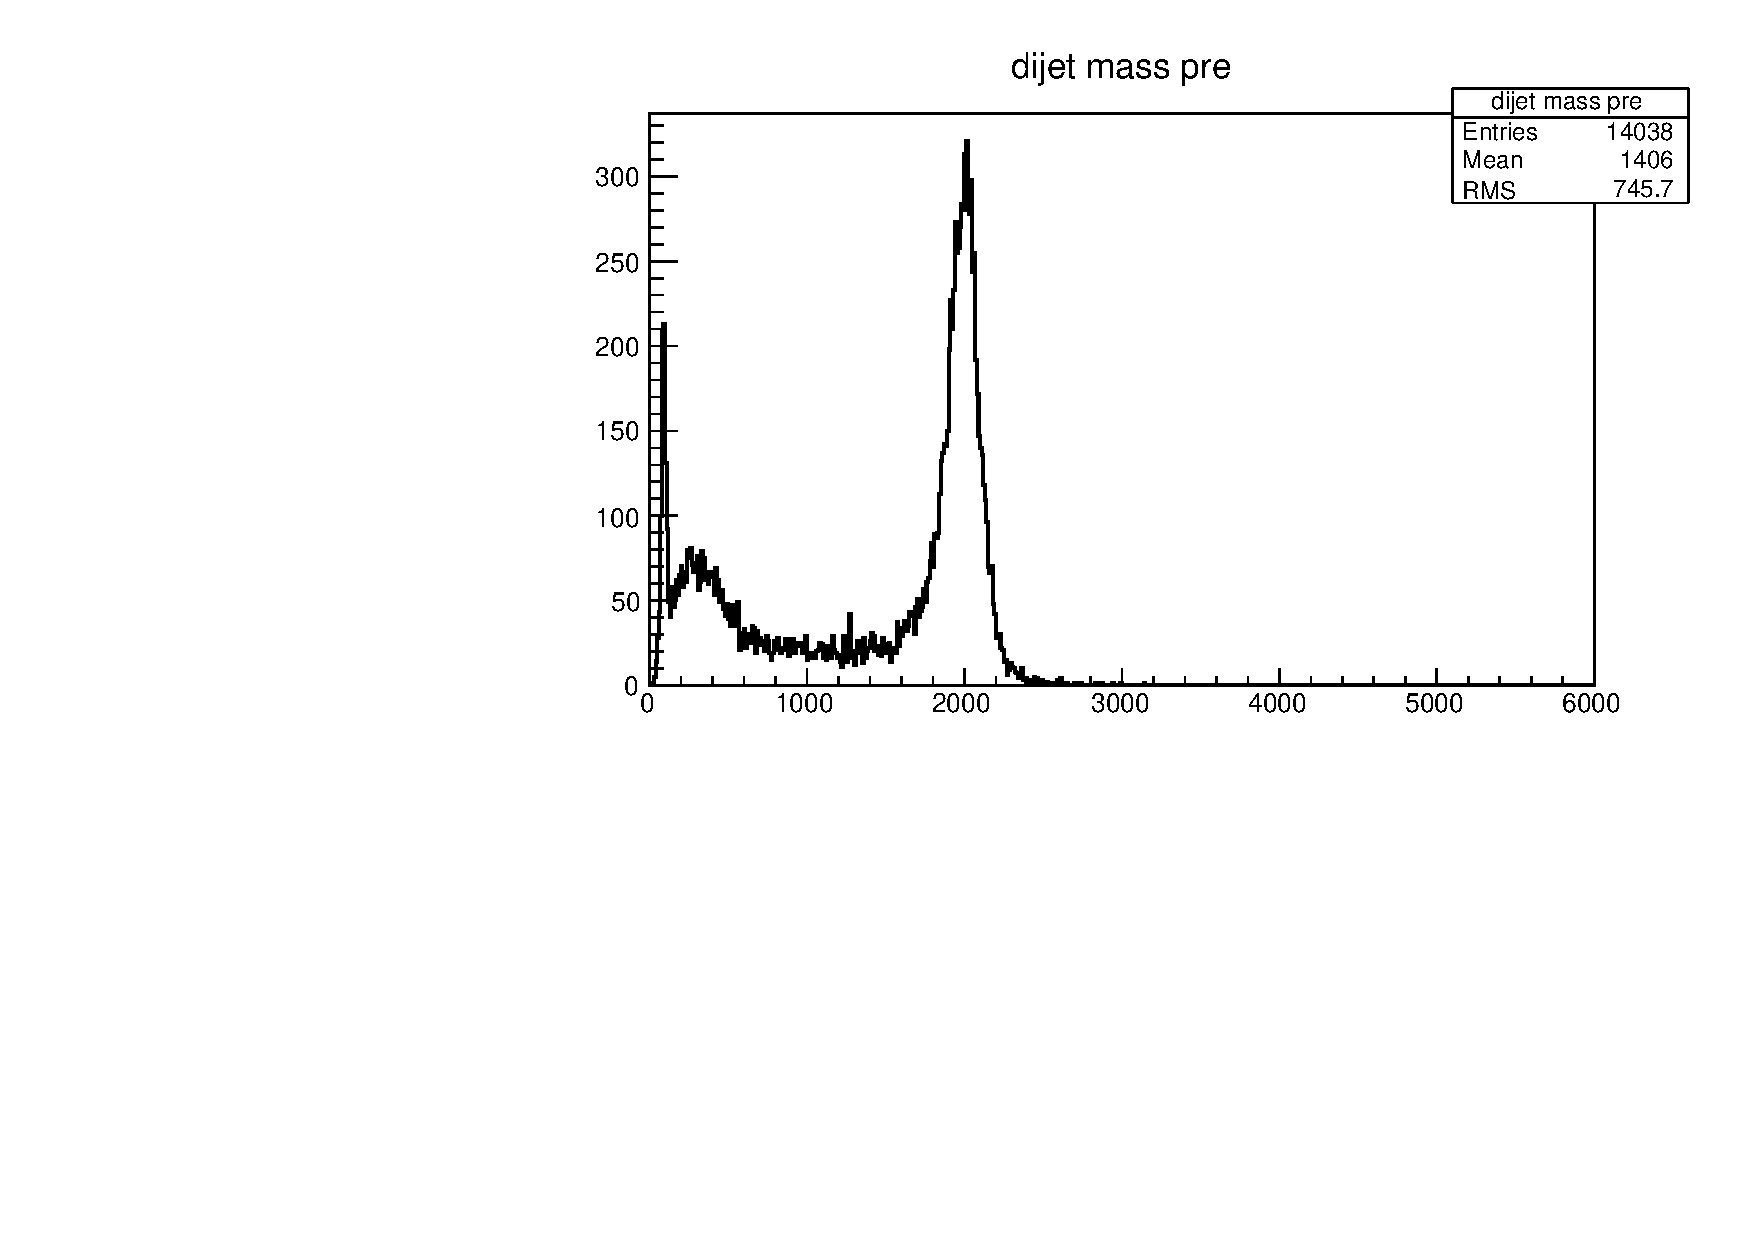
\includegraphics[width=0.48\textwidth]{EXO-12-024/figs/sig-high/Wprime2000-sig-shape.pdf} 
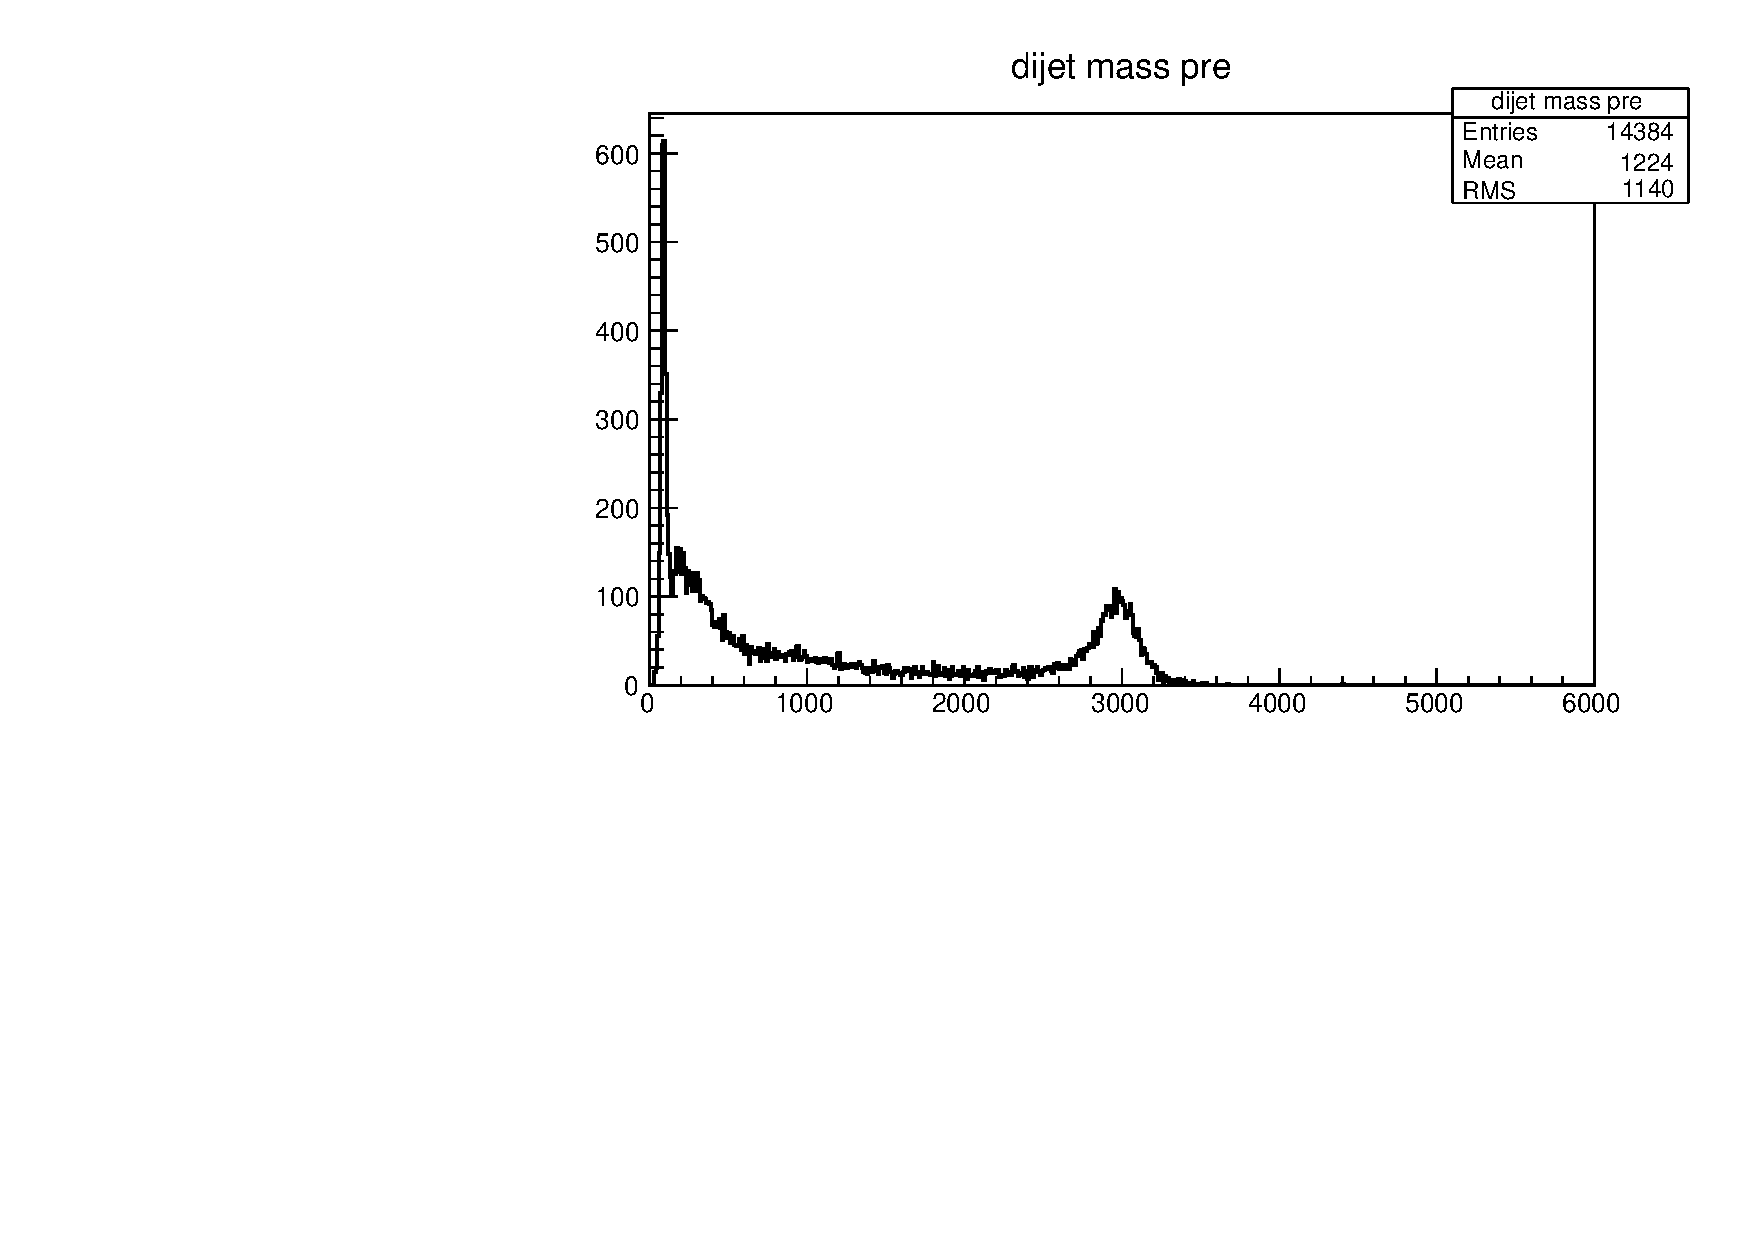
\includegraphics[width=0.48\textwidth]{EXO-12-024/figs/sig-high/Wprime3000-sig-shape.pdf} 
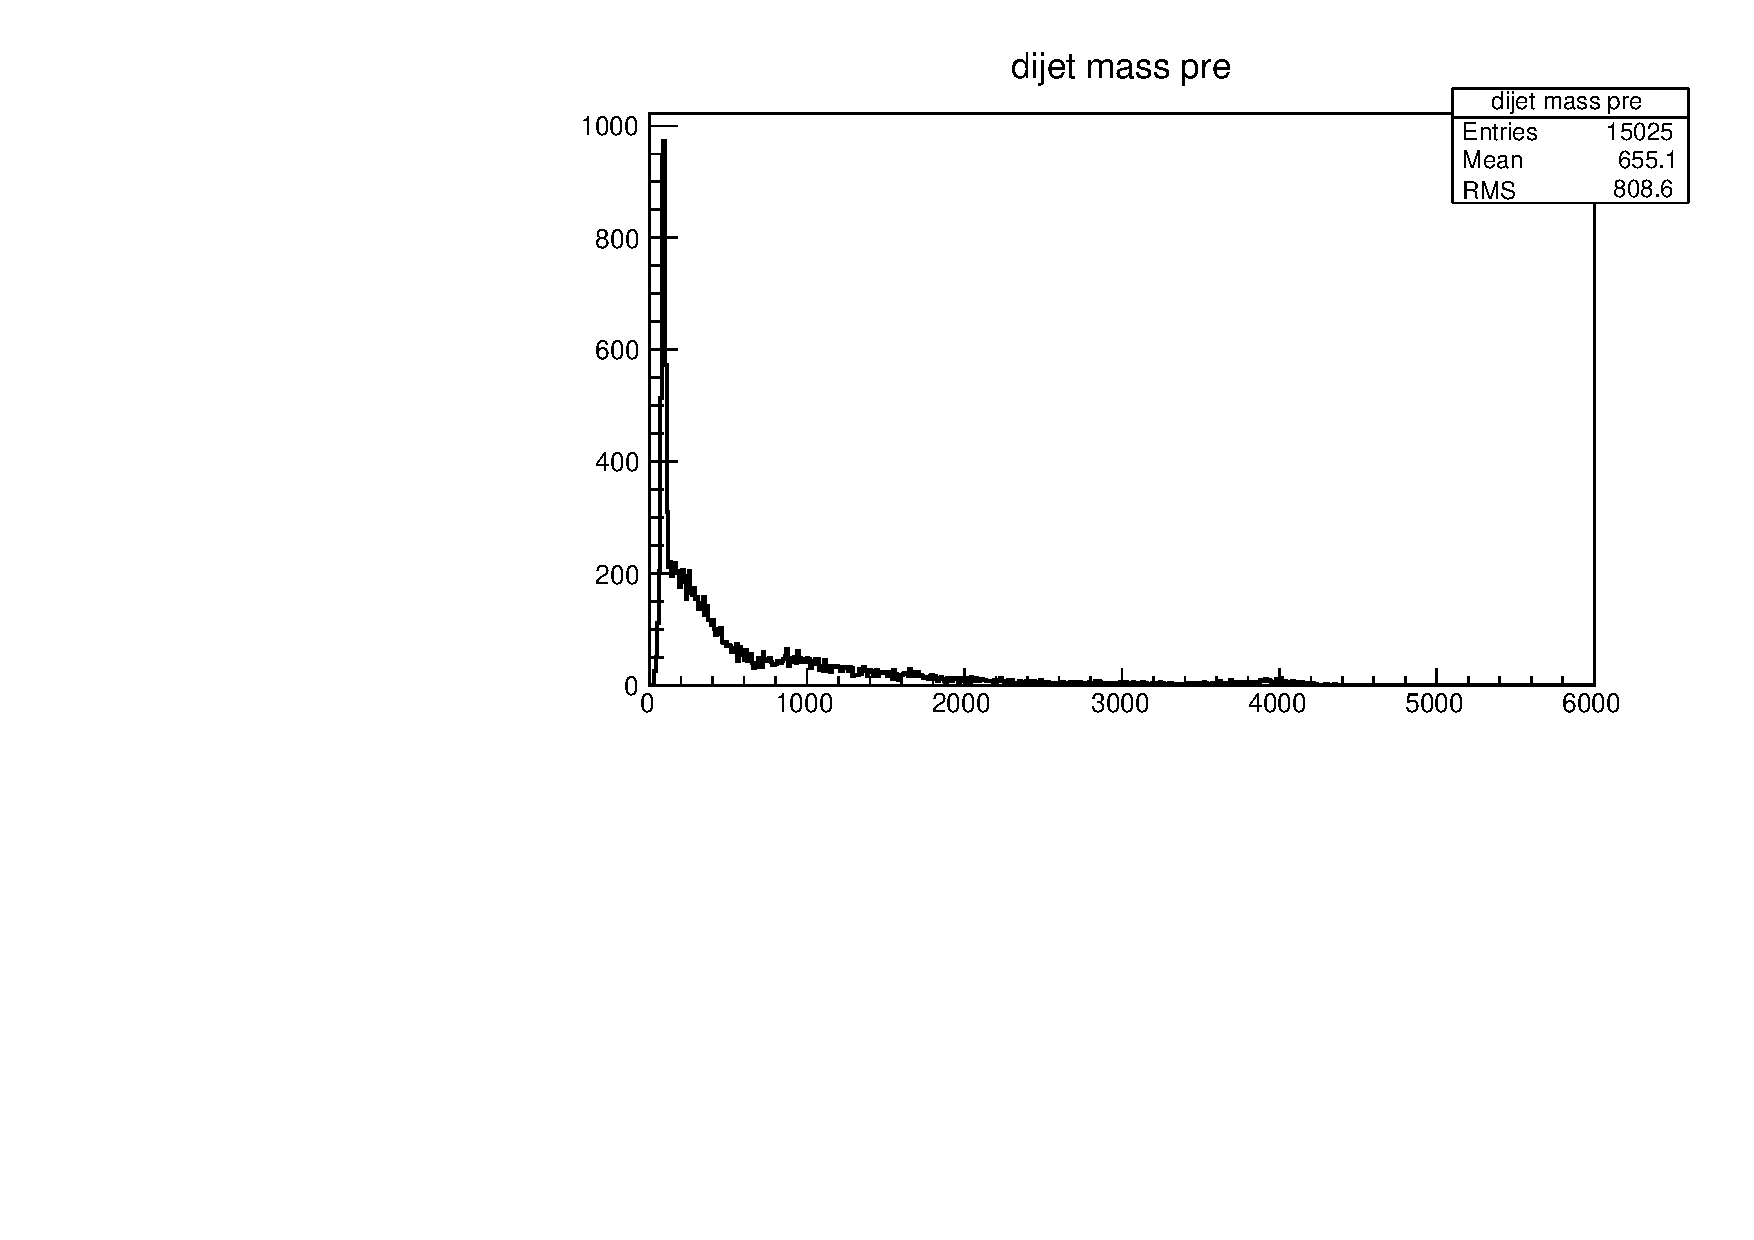
\includegraphics[width=0.48\textwidth]{EXO-12-024/figs/sig-high/Wprime4000-sig-shape-pre.pdf} 
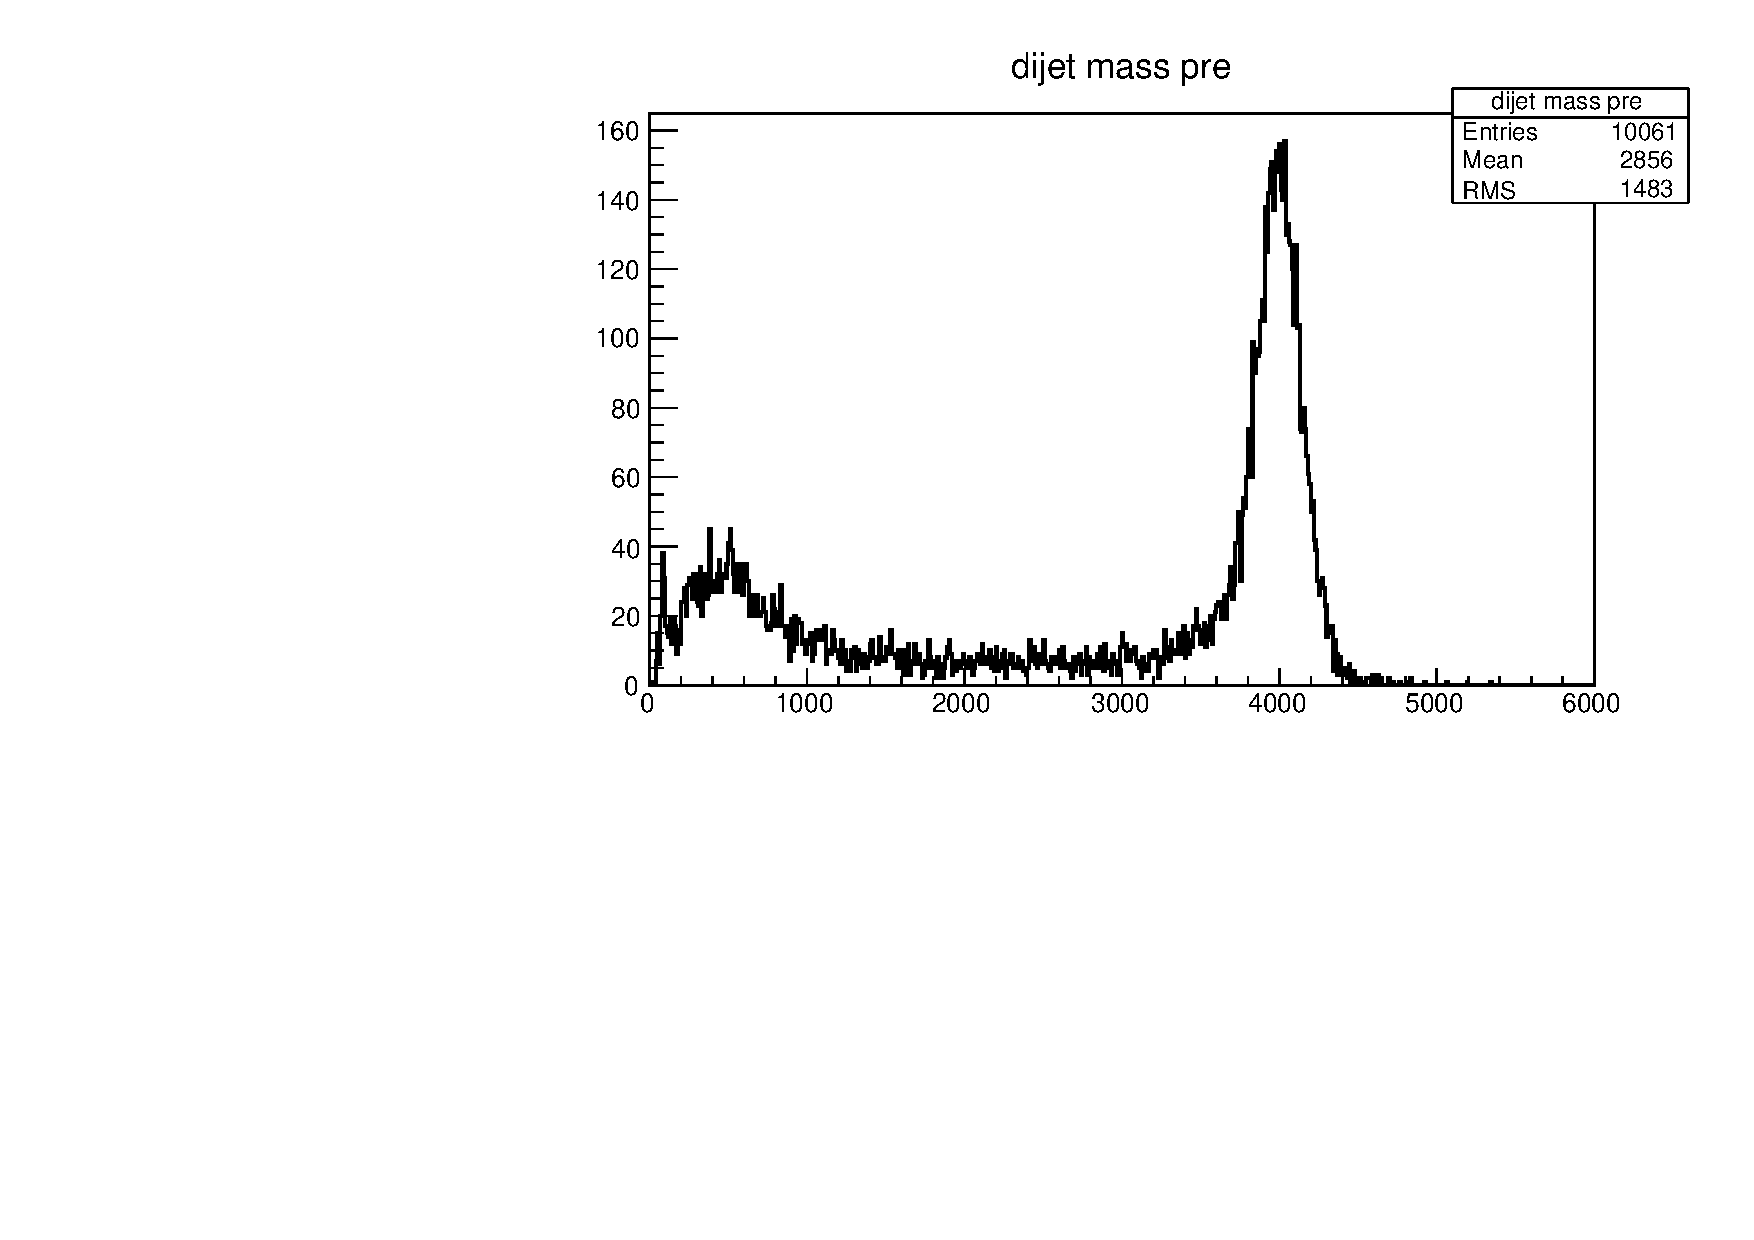
\includegraphics[width=0.48\textwidth]{EXO-12-024/figs/sig-high/RSGWWHerwig4000pre.pdf}
\caption{Comparsion for signal dijet mass distribution for $W' \to WZ$ at 2.0 TeV(top left), 3.0 TeV(top right), 4.0 TeV(bottom left). 
Plot on the right bottom is the dijet mass distribution for $G_{RS} \to WW$ at 4.0 TeV. }
\label{figs:sig-pile-up-dijetmass}
\end{figure}

%\subsection{Tagging efficiency w.r.t jet pt}
%\begin{figure*}[[h!tpb]]
%\centering
%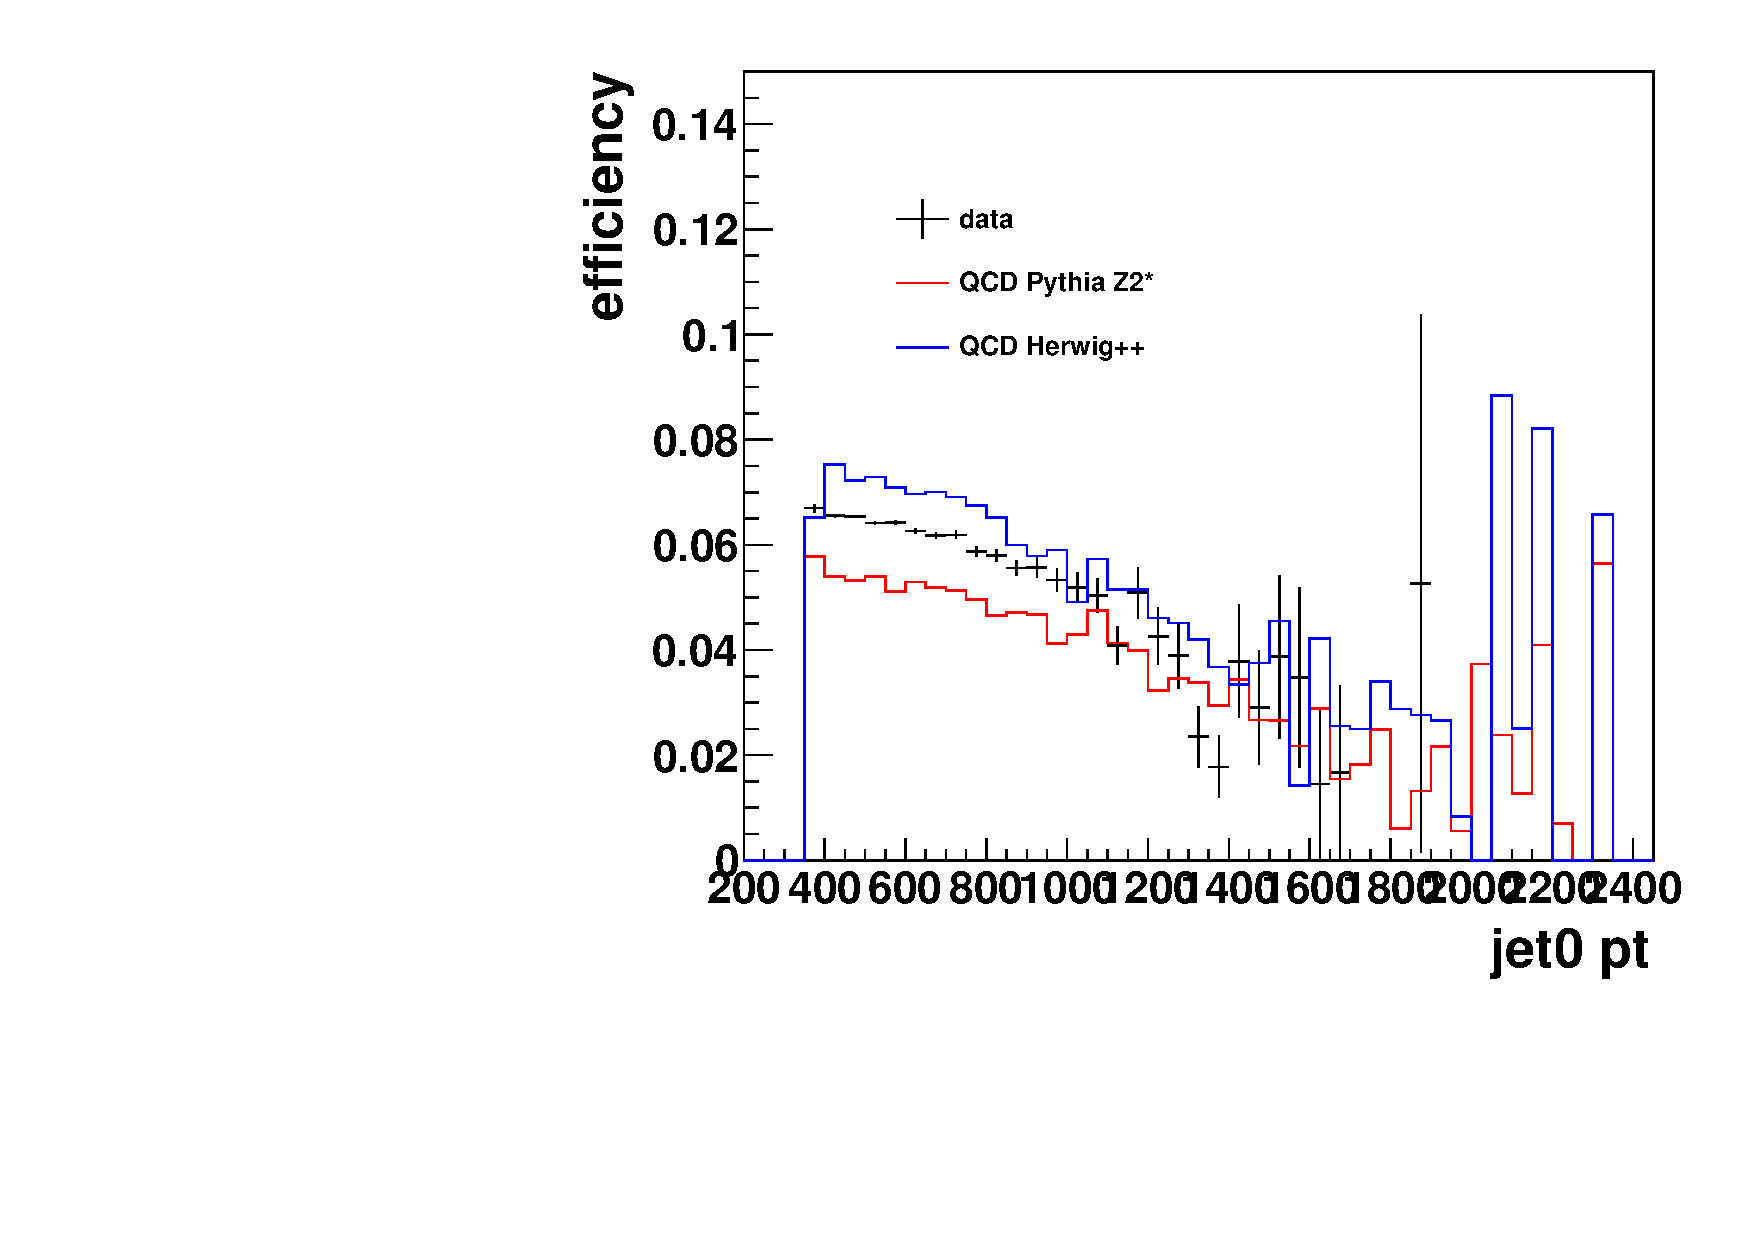
\includegraphics[width=0.48\textwidth]{EXO-12-024/figs/taggingpt/pt0_eff.pdf}
%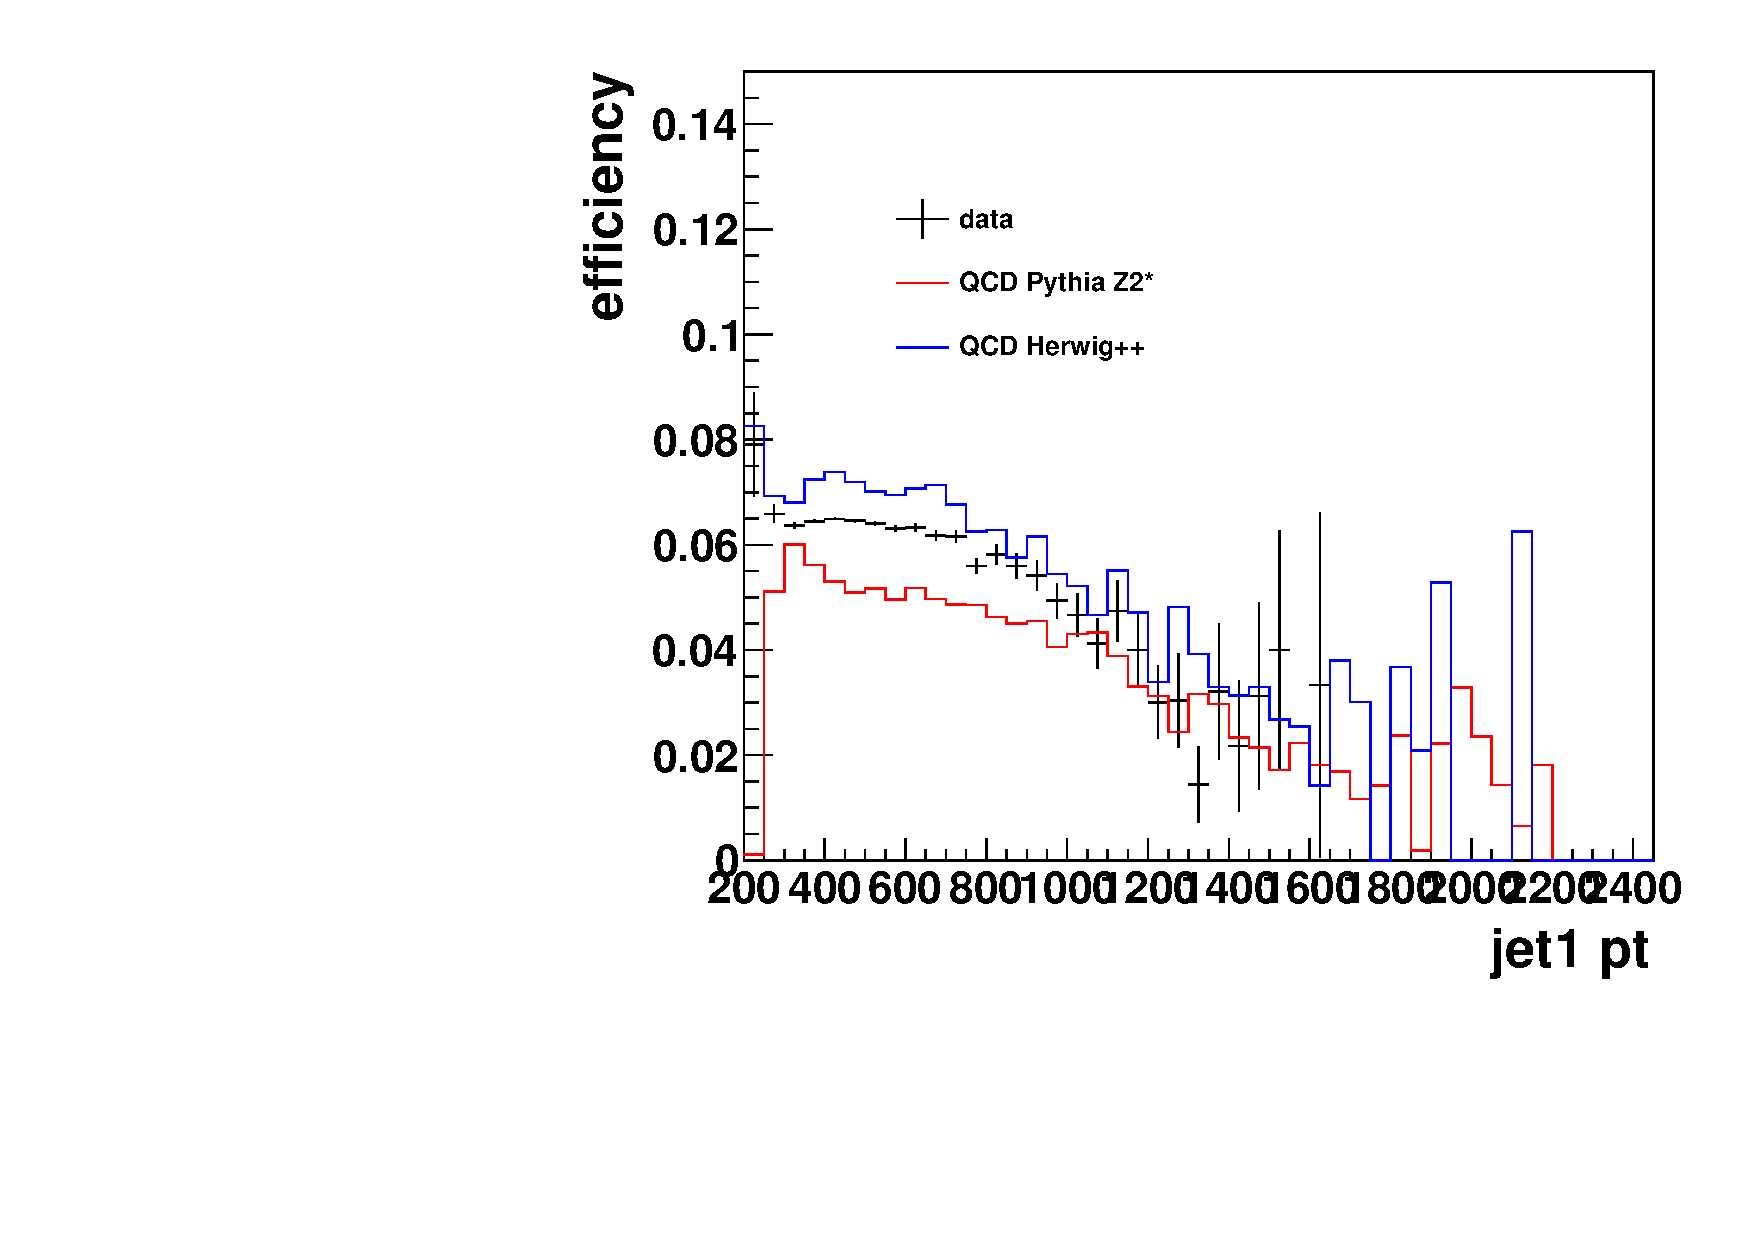
\includegraphics[width=0.48\textwidth]{EXO-12-024/figs/taggingpt/pt1_eff.pdf}
%\caption{Tagging efficiency of tagging leading jet only w.r.t to leading jet pt.Plot on the right is for the
%second leading jet.}
%\label{figs:sig-pile-up-dijetmass}
%\end{figure*}

\clearpage

\section{Event displays}
\label{appendix:events}
%\begin{figure}[htb]
%\begin{center}
%\includegraphics[width=0.8\textwidth,angle=0]{EXO-12-024/figs/event-display/pteven2-177074_1171400298_711_3DTower.pdf}
%\includegraphics[width=0.8\textwidth,angle=0]{EXO-12-024/figs/event-display/pteven2-177074_1171400298_711_Lego.pdf}
%\end{center}
%\caption{Event display of a nicely balanced double W/Z-tagged event with a dijet invariant mass of 1.043~\TeVcc .
%The transverse momenta of the two leading jets are 0.538~\TeVcc and 0.476~\TeVcc .
%The invariant mass of the two leading pruned CA8 jets is 94.41 \GeVcc and 80.75 \GeVcc .
%}
%\label{fig:eventdisplay1}
%\end{figure}

\begin{figure}[htb]
\begin{center}
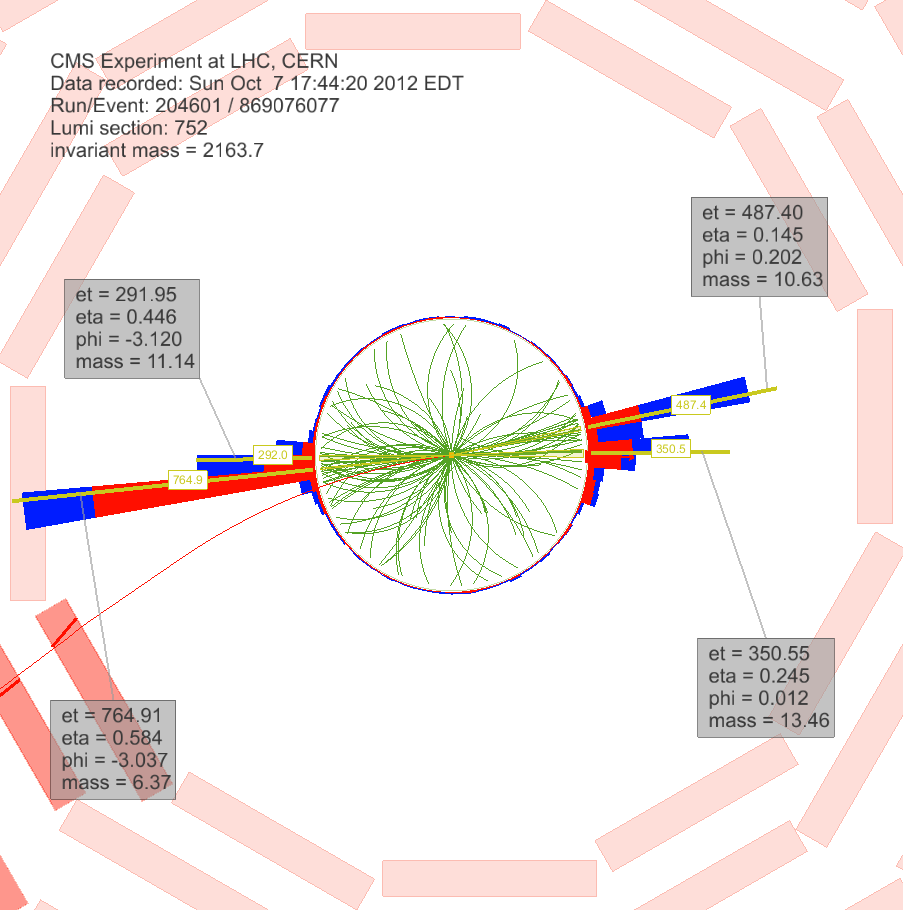
\includegraphics[width=0.6\textwidth,angle=0]{EXO-12-024/figs/event-display/highdoublemass/rho-phi-white.png}
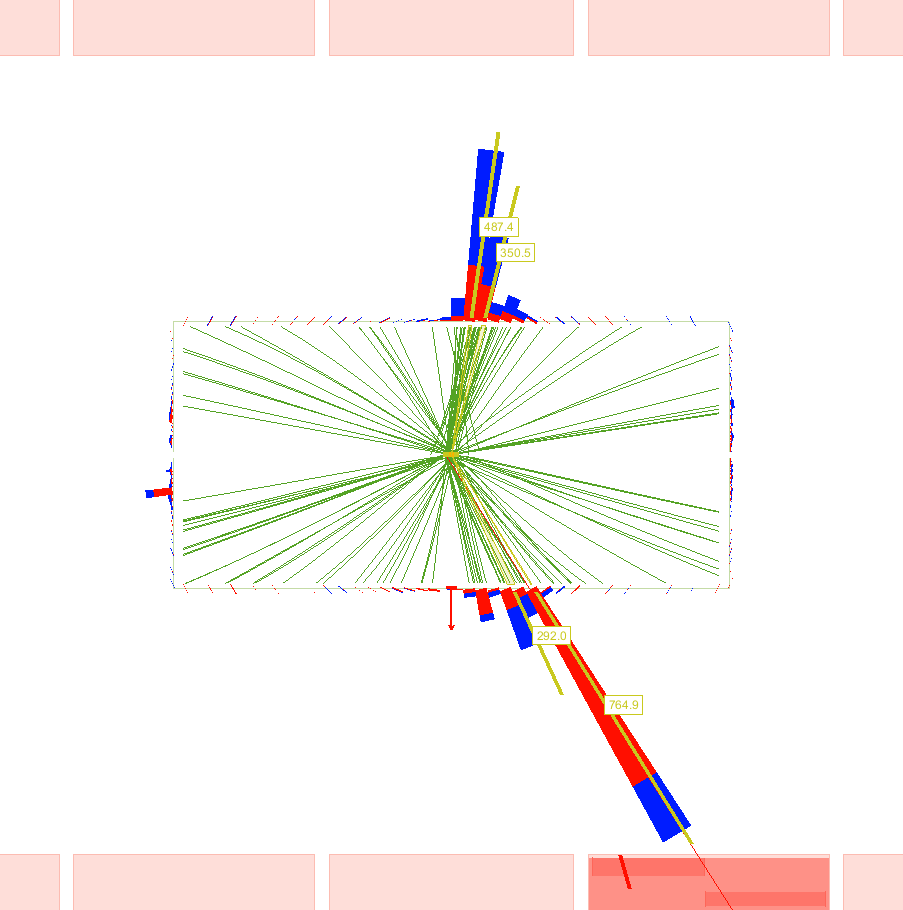
\includegraphics[width=0.6\textwidth,angle=0]{EXO-12-024/figs/event-display/highdoublemass/rho-z-white.png}
\end{center}
\caption{Event display of double W/Z-tagged event with the highest dijet invariant mass of 2.16~\TeVcc .
The transverse momenta of the two leading jets are 1.1~\TeVcc and 0.92~\TeVcc .
The invariant mass of the two leading pruned CA8 jets is 97.82 \GeVcc and 85.08 \GeVcc .
}
\label{fig:eventdisplay1}
\end{figure}

\begin{figure}[htb]
\begin{center}
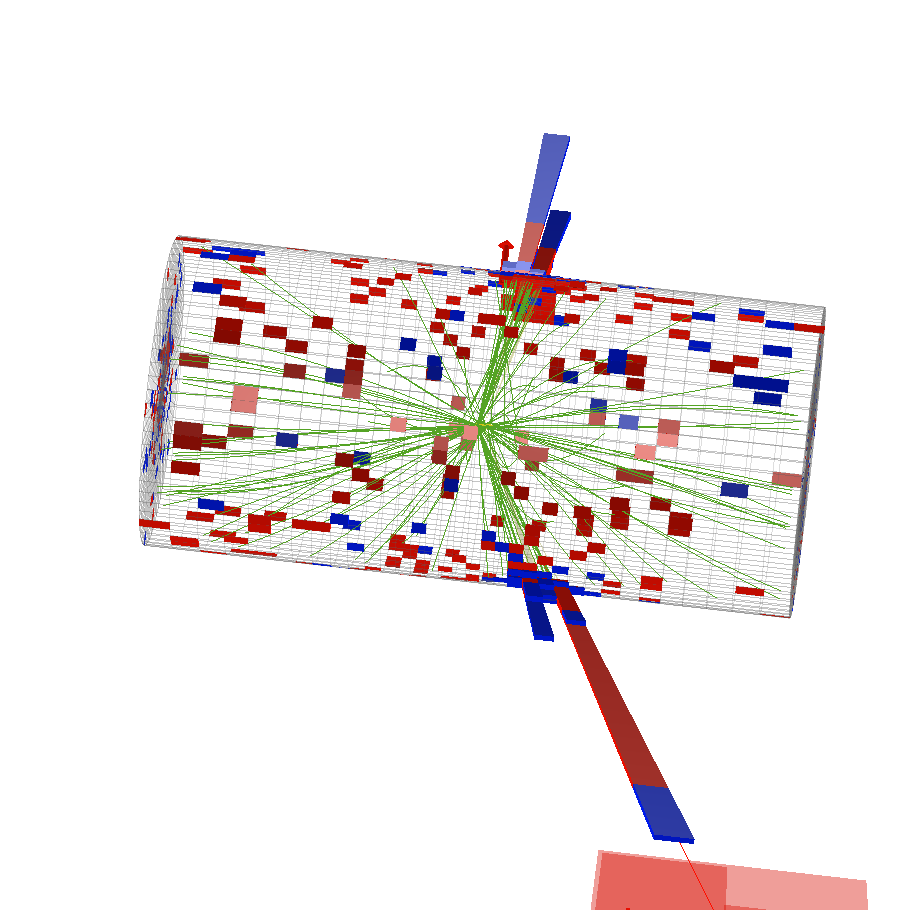
\includegraphics[width=0.6\textwidth,angle=0]{EXO-12-024/figs/event-display/highdoublemass/tower-white.png}
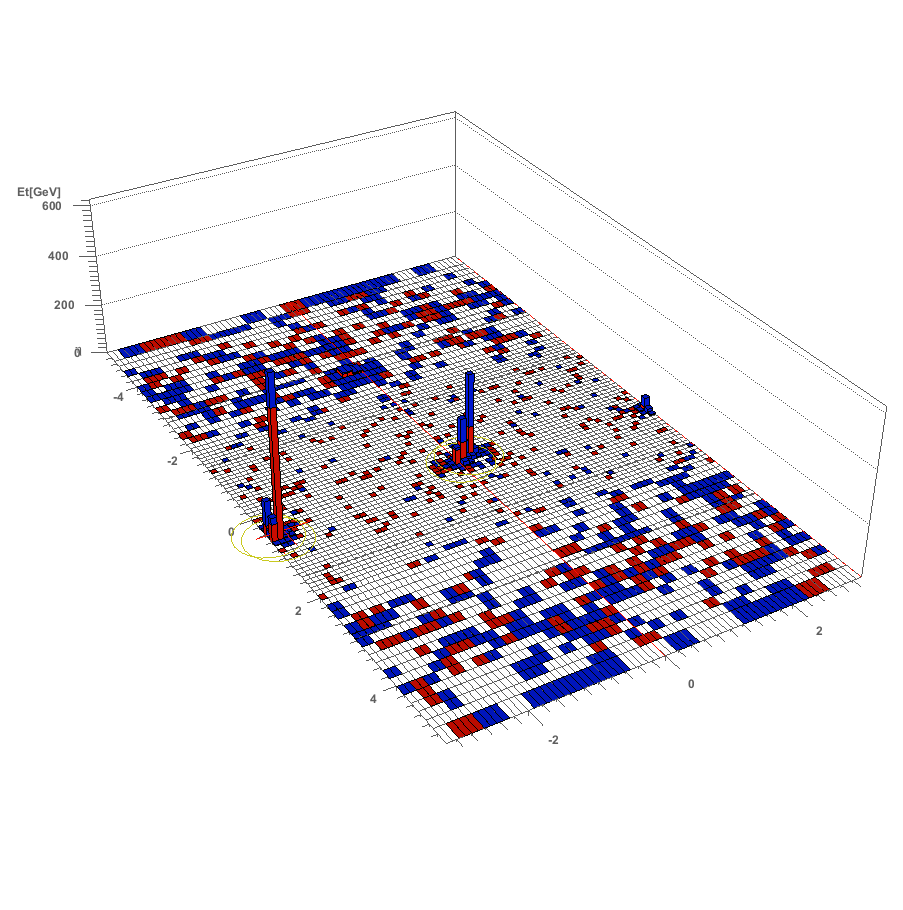
\includegraphics[width=0.6\textwidth,angle=0]{EXO-12-024/figs/event-display/highdoublemass/lego-white.png}
\end{center}
\caption{Event display of double W/Z-tagged event with the highest dijet invariant mass of 2.16~\TeVcc .
The transverse momenta of the two leading jets are 1.1~\TeVcc and 0.92~\TeVcc .
The invariant mass of the two leading pruned CA8 jets is 97.82 \GeVcc and 85.08 \GeVcc .
}
\label{fig:eventdisplay2}
\end{figure}

\begin{figure}[htb]
\begin{center}
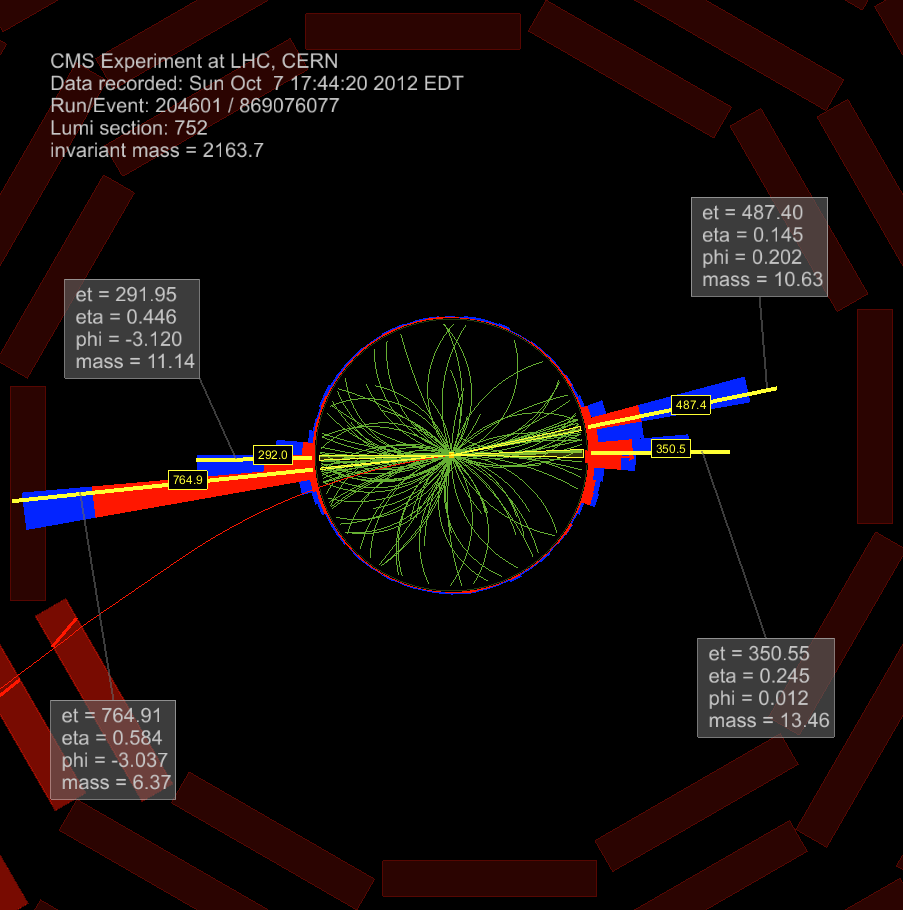
\includegraphics[width=0.6\textwidth,angle=0]{EXO-12-024/figs/event-display/highdoublemass/rho-phi-black.png}
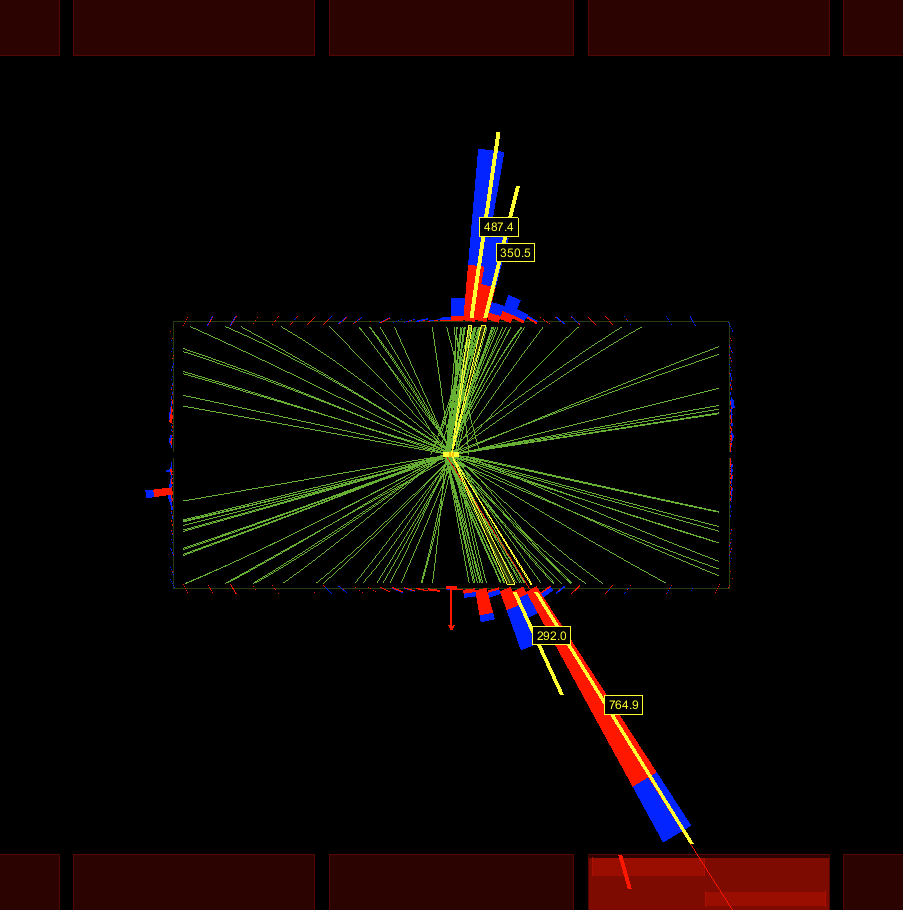
\includegraphics[width=0.6\textwidth,angle=0]{EXO-12-024/figs/event-display/highdoublemass/rho-z-black.png}
\end{center}
\caption{Event display of double W/Z-tagged event with the highest dijet invariant mass of 2.16~\TeVcc .
The transverse momenta of the two leading jets are 1.1~\TeVcc and 0.92~\TeVcc .
The invariant mass of the two leading pruned CA8 jets is 97.82 \GeVcc and 85.08 \GeVcc .
}
\label{fig:eventdisplay3}
\end{figure}

\begin{figure}[htb]
\begin{center}
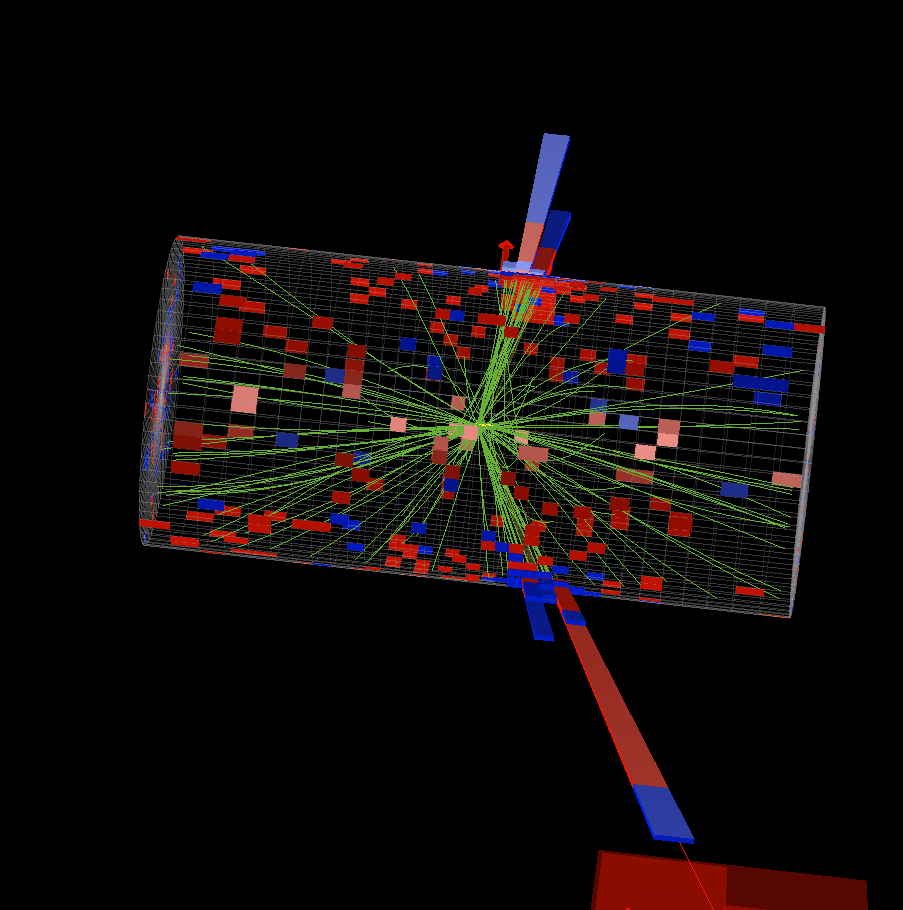
\includegraphics[width=0.6\textwidth,angle=0]{EXO-12-024/figs/event-display/highdoublemass/tower-black.png}
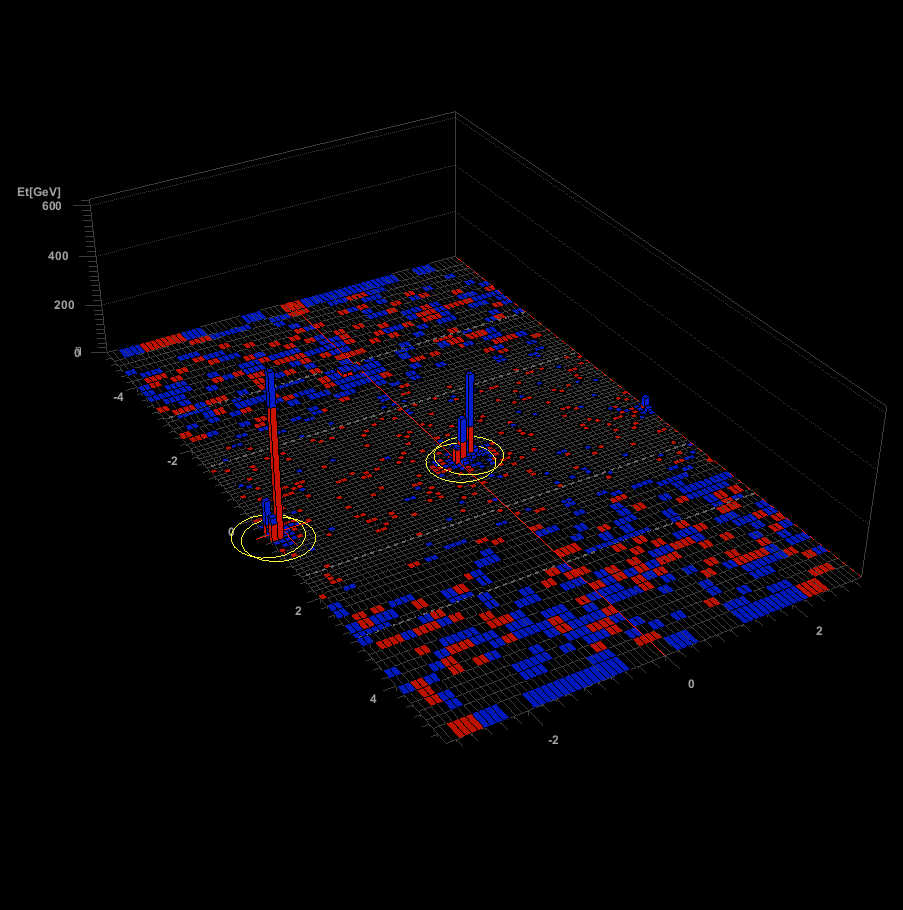
\includegraphics[width=0.6\textwidth,angle=0]{EXO-12-024/figs/event-display/highdoublemass/lego-black.png}
\end{center}
\caption{Event display of double W/Z-tagged event with the highest dijet invariant mass of 2.16~\TeVcc .
The transverse momenta of the two leading jets are 1.1~\TeVcc and 0.92~\TeVcc .
The invariant mass of the two leading pruned CA8 jets is 97.82 \GeVcc and 85.08 \GeVcc .
}
\label{fig:eventdisplay4}
\end{figure}

\begin{figure}[htb]
\begin{center}
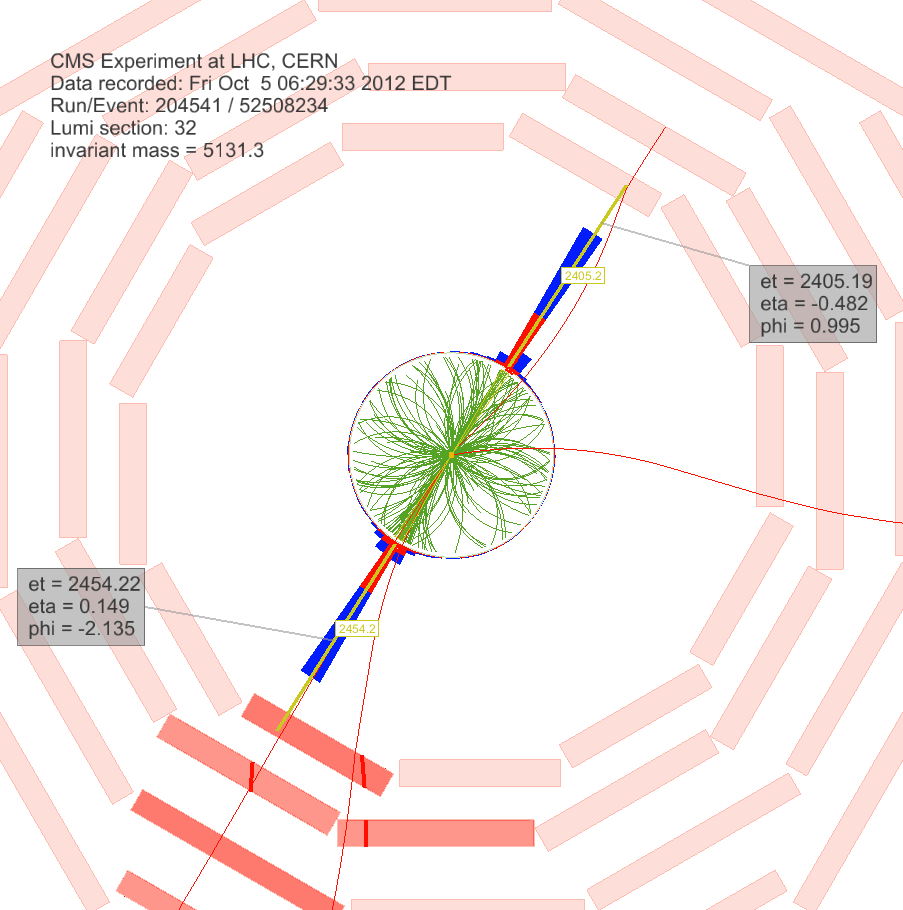
\includegraphics[width=0.6\textwidth,angle=0]{EXO-12-024/figs/event-display/prehighest/rho-phi-white.png}
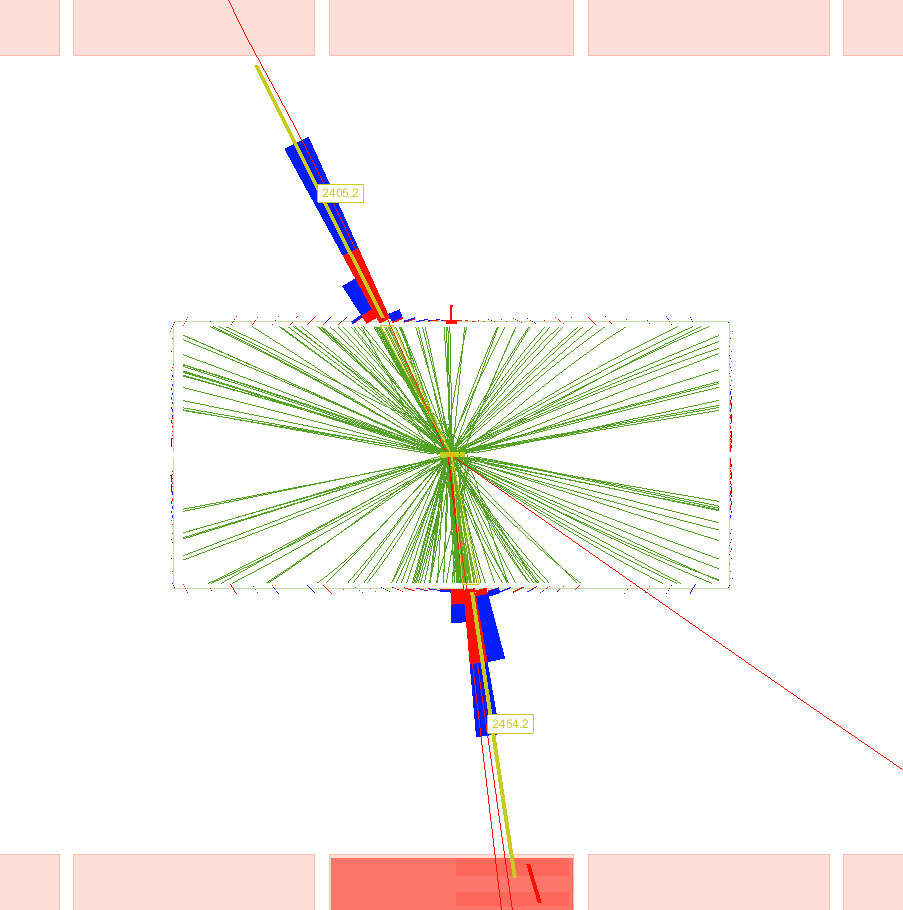
\includegraphics[width=0.6\textwidth,angle=0]{EXO-12-024/figs/event-display/prehighest/rho-z-white.png}
\end{center}
\caption{Event display of event with the highest dijet invariant mass of 5.13~\TeVcc .
The transverse momenta of the two leading AK5 jets are 2.45~\TeVcc and 2.40~\TeVcc .
}
\label{fig:eventdisplay11}
\end{figure}

\begin{figure}[htb]
\begin{center}
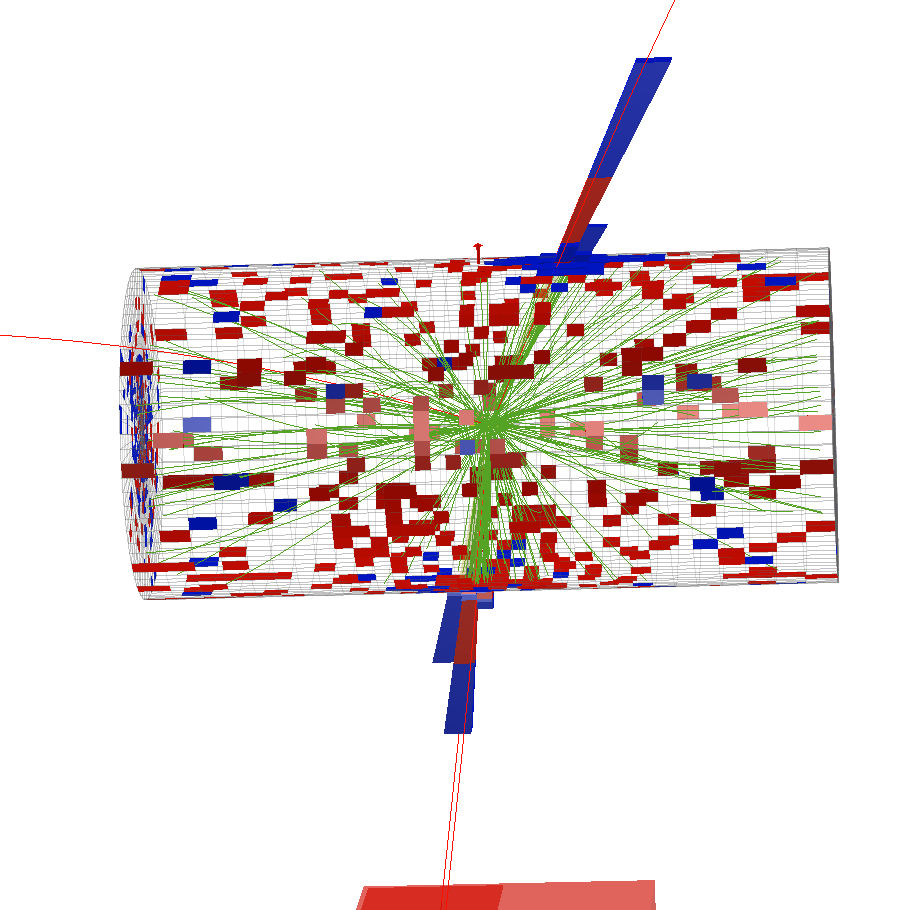
\includegraphics[width=0.6\textwidth,angle=0]{EXO-12-024/figs/event-display/prehighest/tower-white.png}
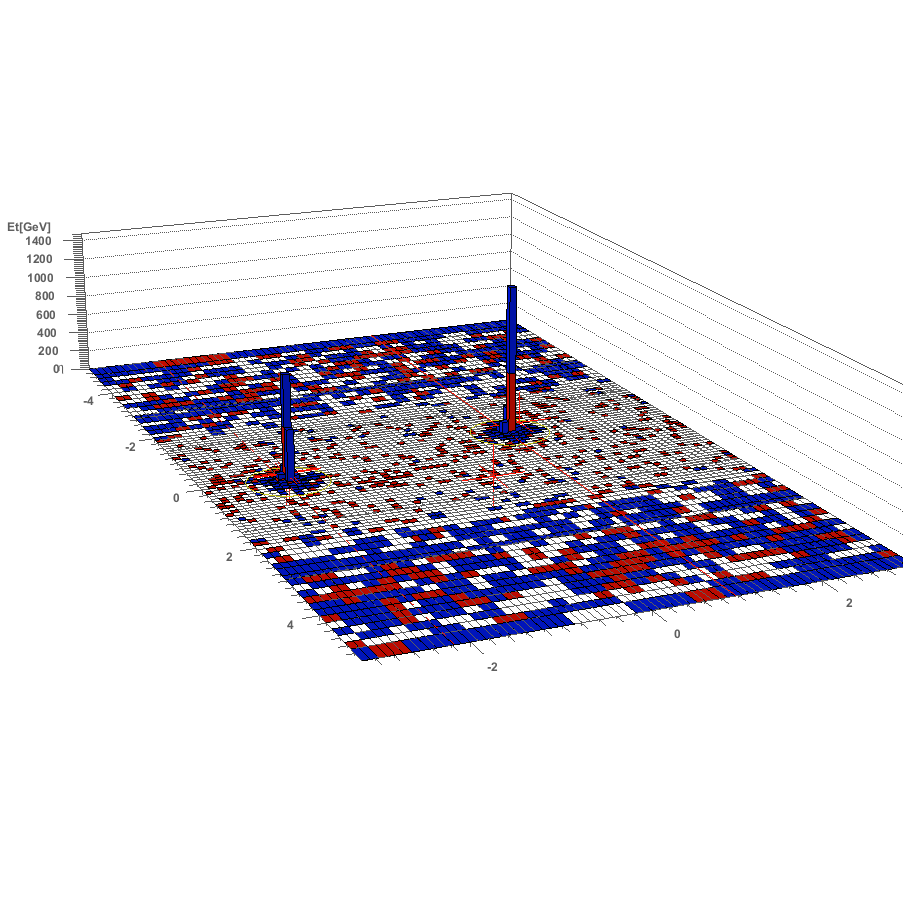
\includegraphics[width=0.6\textwidth,angle=0]{EXO-12-024/figs/event-display/prehighest/lego-white.png}
\end{center}
\caption{Event display of event with the highest dijet invariant mass of 5.13~\TeVcc .
The transverse momenta of the two leading AK5 jets are 2.45~\TeVcc and 2.40~\TeVcc .
}
\label{fig:eventdisplay12}
\end{figure}

\begin{figure}[htb]
\begin{center}
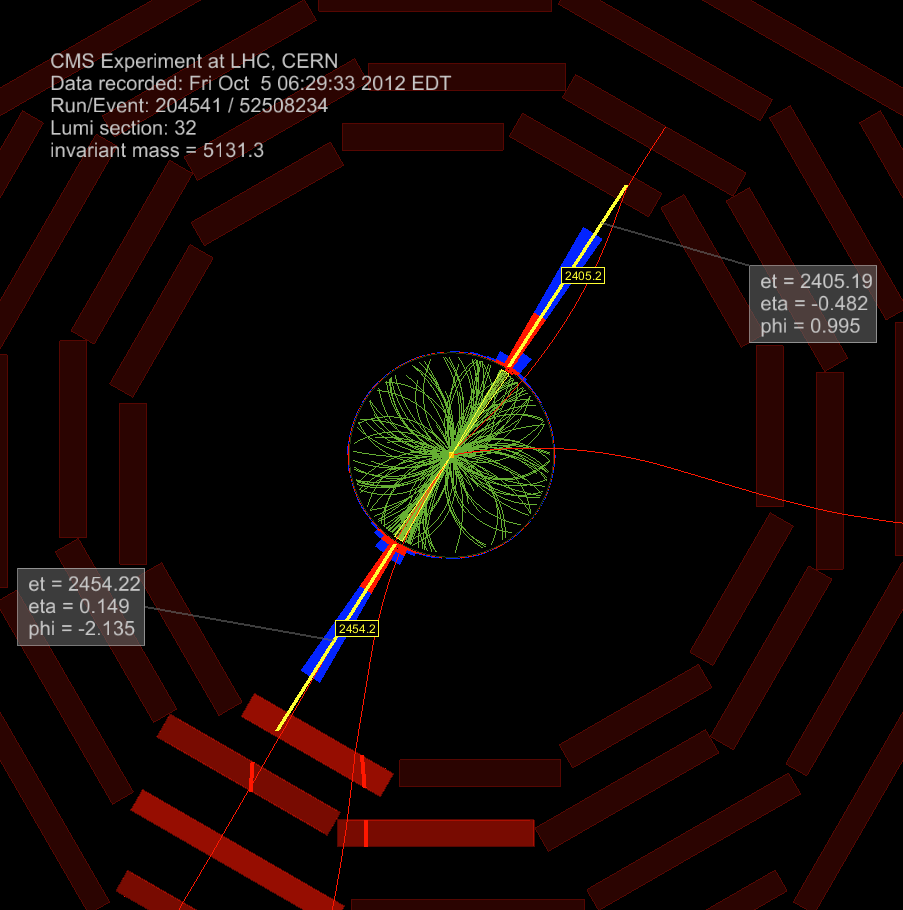
\includegraphics[width=0.6\textwidth,angle=0]{EXO-12-024/figs/event-display/prehighest/rho-phi-black.png}
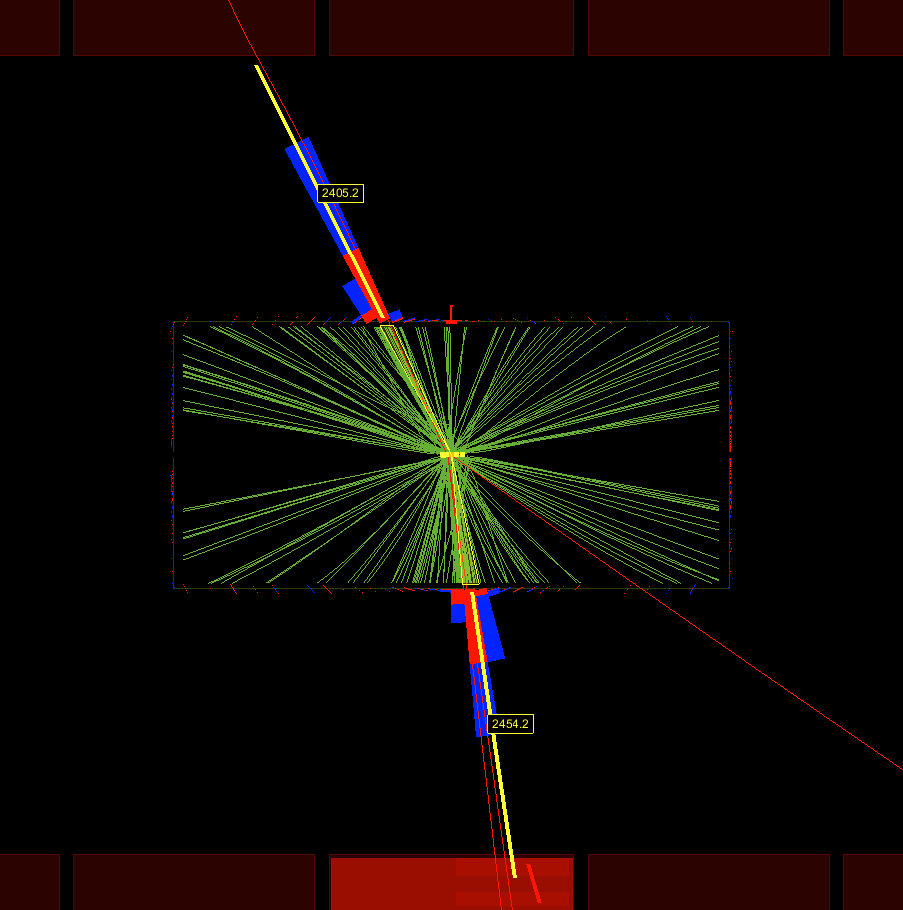
\includegraphics[width=0.6\textwidth,angle=0]{EXO-12-024/figs/event-display/prehighest/rho-z-black.png}
\end{center}
\caption{Event display of event with the highest dijet invariant mass of 5.13~\TeVcc .
The transverse momenta of the two leading AK5 jets are 2.45~\TeVcc and 2.40~\TeVcc .
}
\label{fig:eventdisplay13}
\end{figure}

\begin{figure}[htb]
\begin{center}
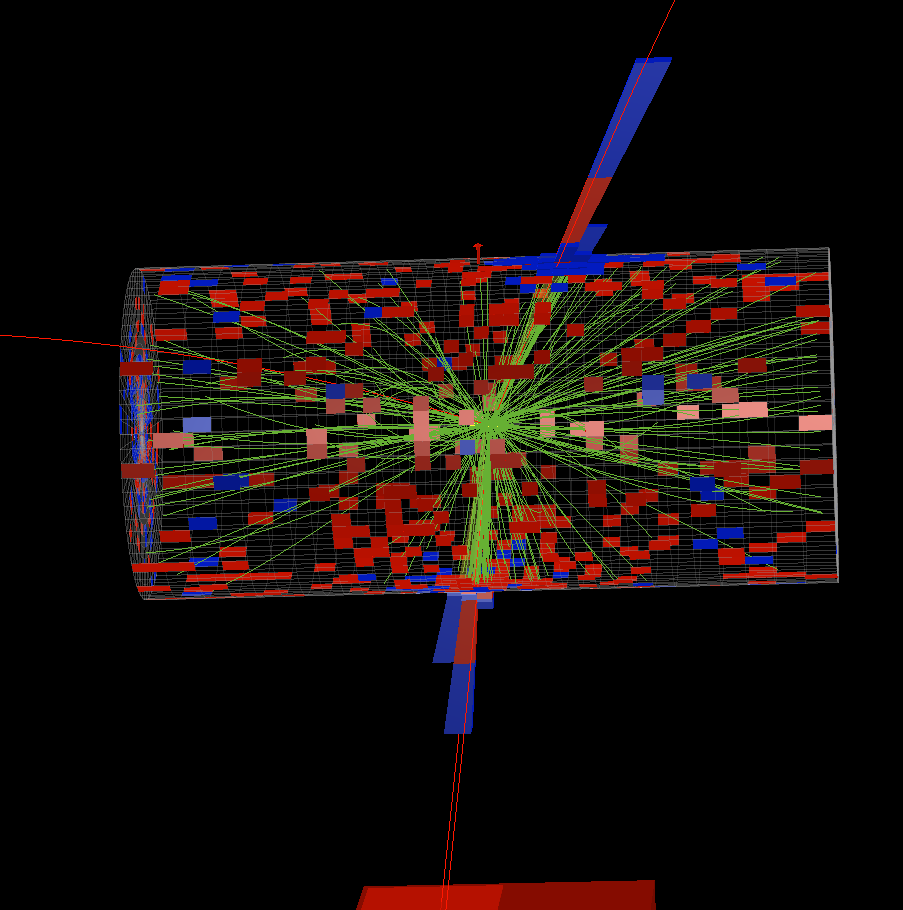
\includegraphics[width=0.6\textwidth,angle=0]{EXO-12-024/figs/event-display/prehighest/tower-black.png}
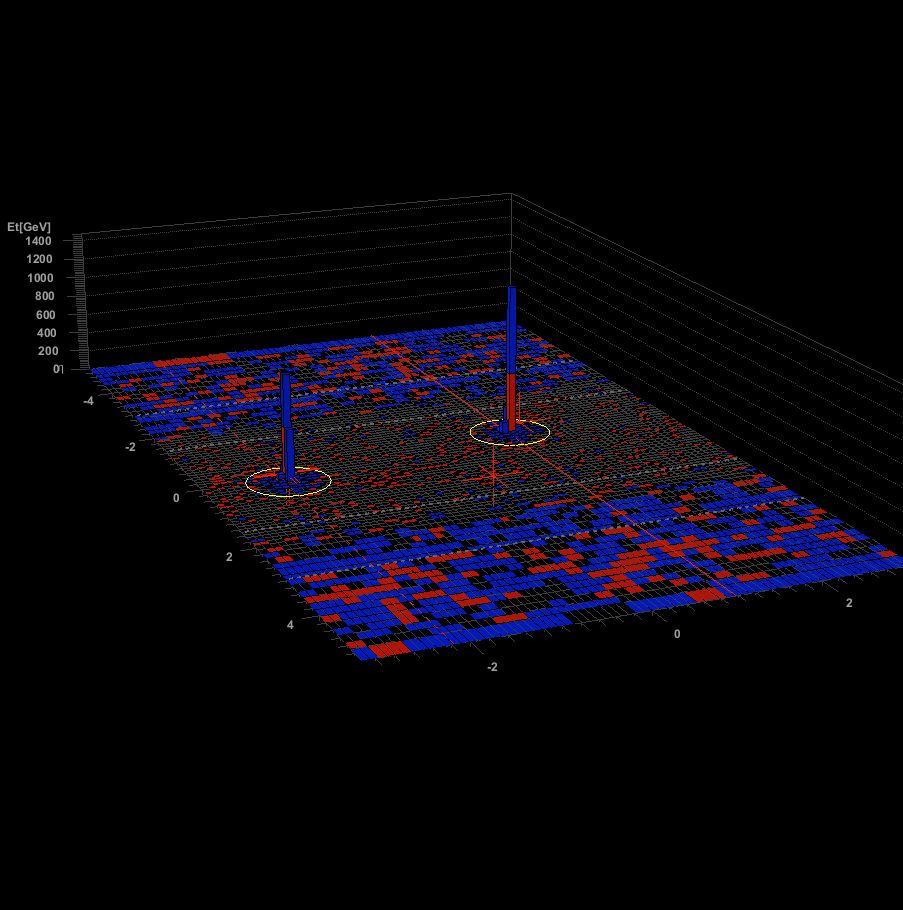
\includegraphics[width=0.6\textwidth,angle=0]{EXO-12-024/figs/event-display/prehighest/lego-black.png}
\end{center}
\caption{Event display of event with the highest dijet invariant mass of 5.13~\TeVcc .
The transverse momenta of the two leading AK5 jets are 2.45~\TeVcc and 2.40~\TeVcc .
}
\label{fig:eventdisplay14}
\end{figure}

\clearpage

%\subsection{Cross checks for the bump at 2 TeV}

%\begin{figure}[htb]
%\begin{center}
%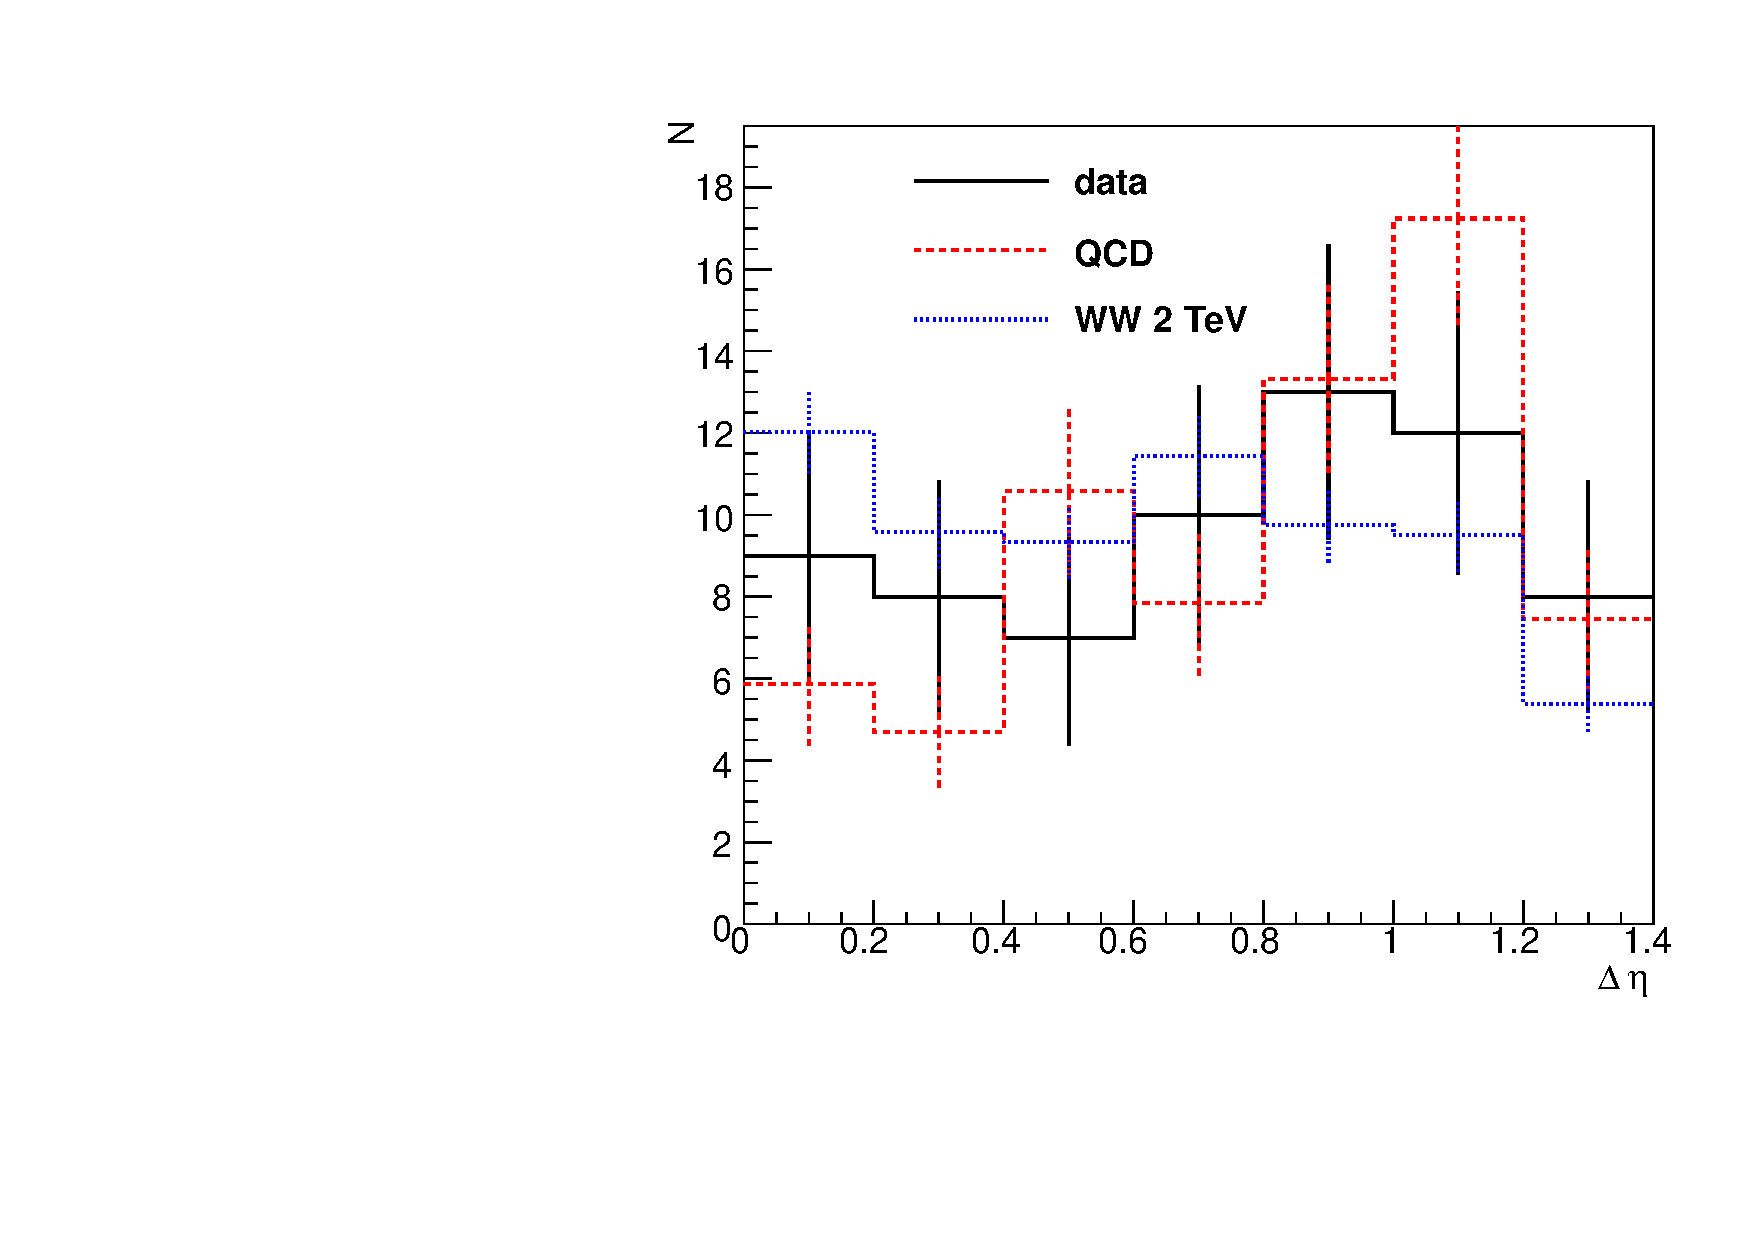
\includegraphics[width=0.48\textwidth,angle=0]{EXO-12-024/figs/appendix/data2012_v3_deta_2mtag_2mdtag_deta.pdf}
%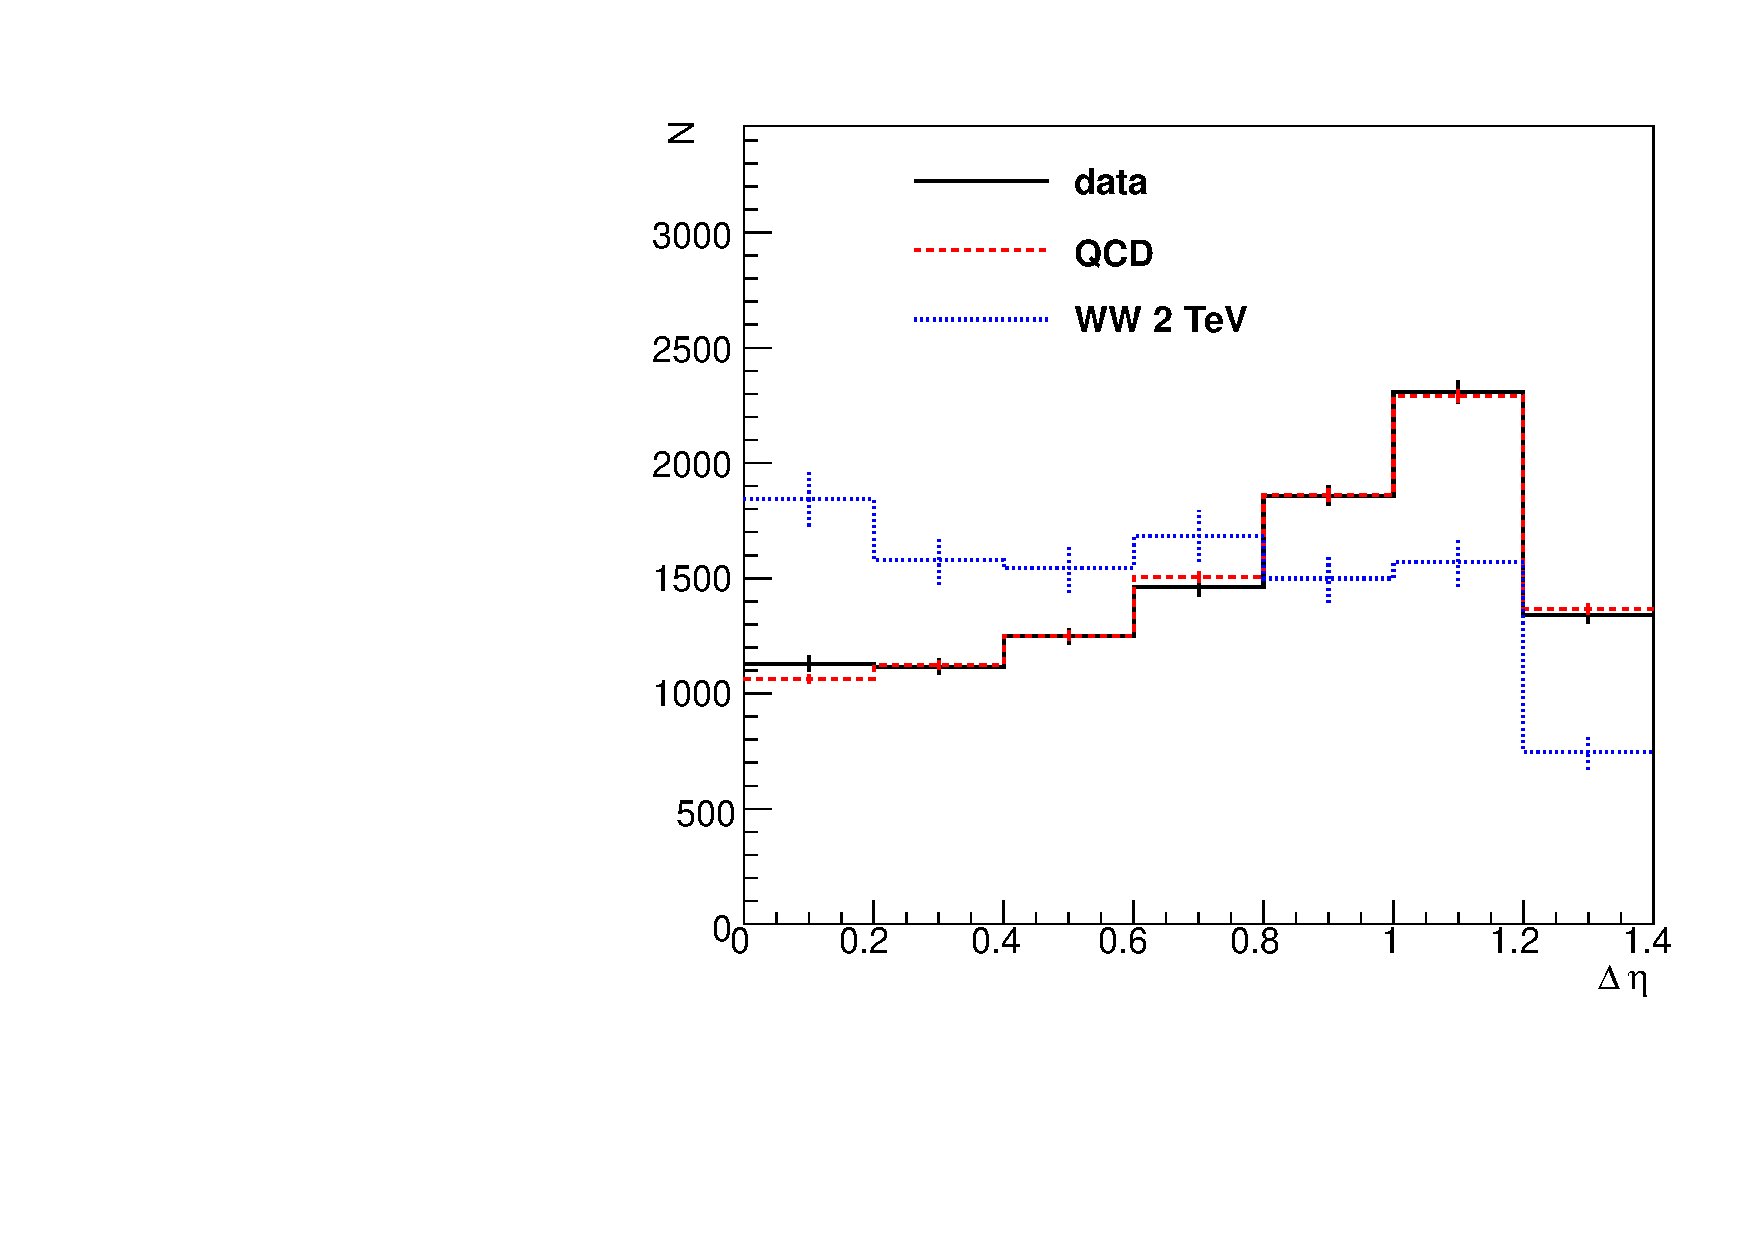
\includegraphics[width=0.48\textwidth,angle=0]{EXO-12-024/figs/appendix/data2012_v3_deta_1mtag_0mdtag_deta.pdf}
%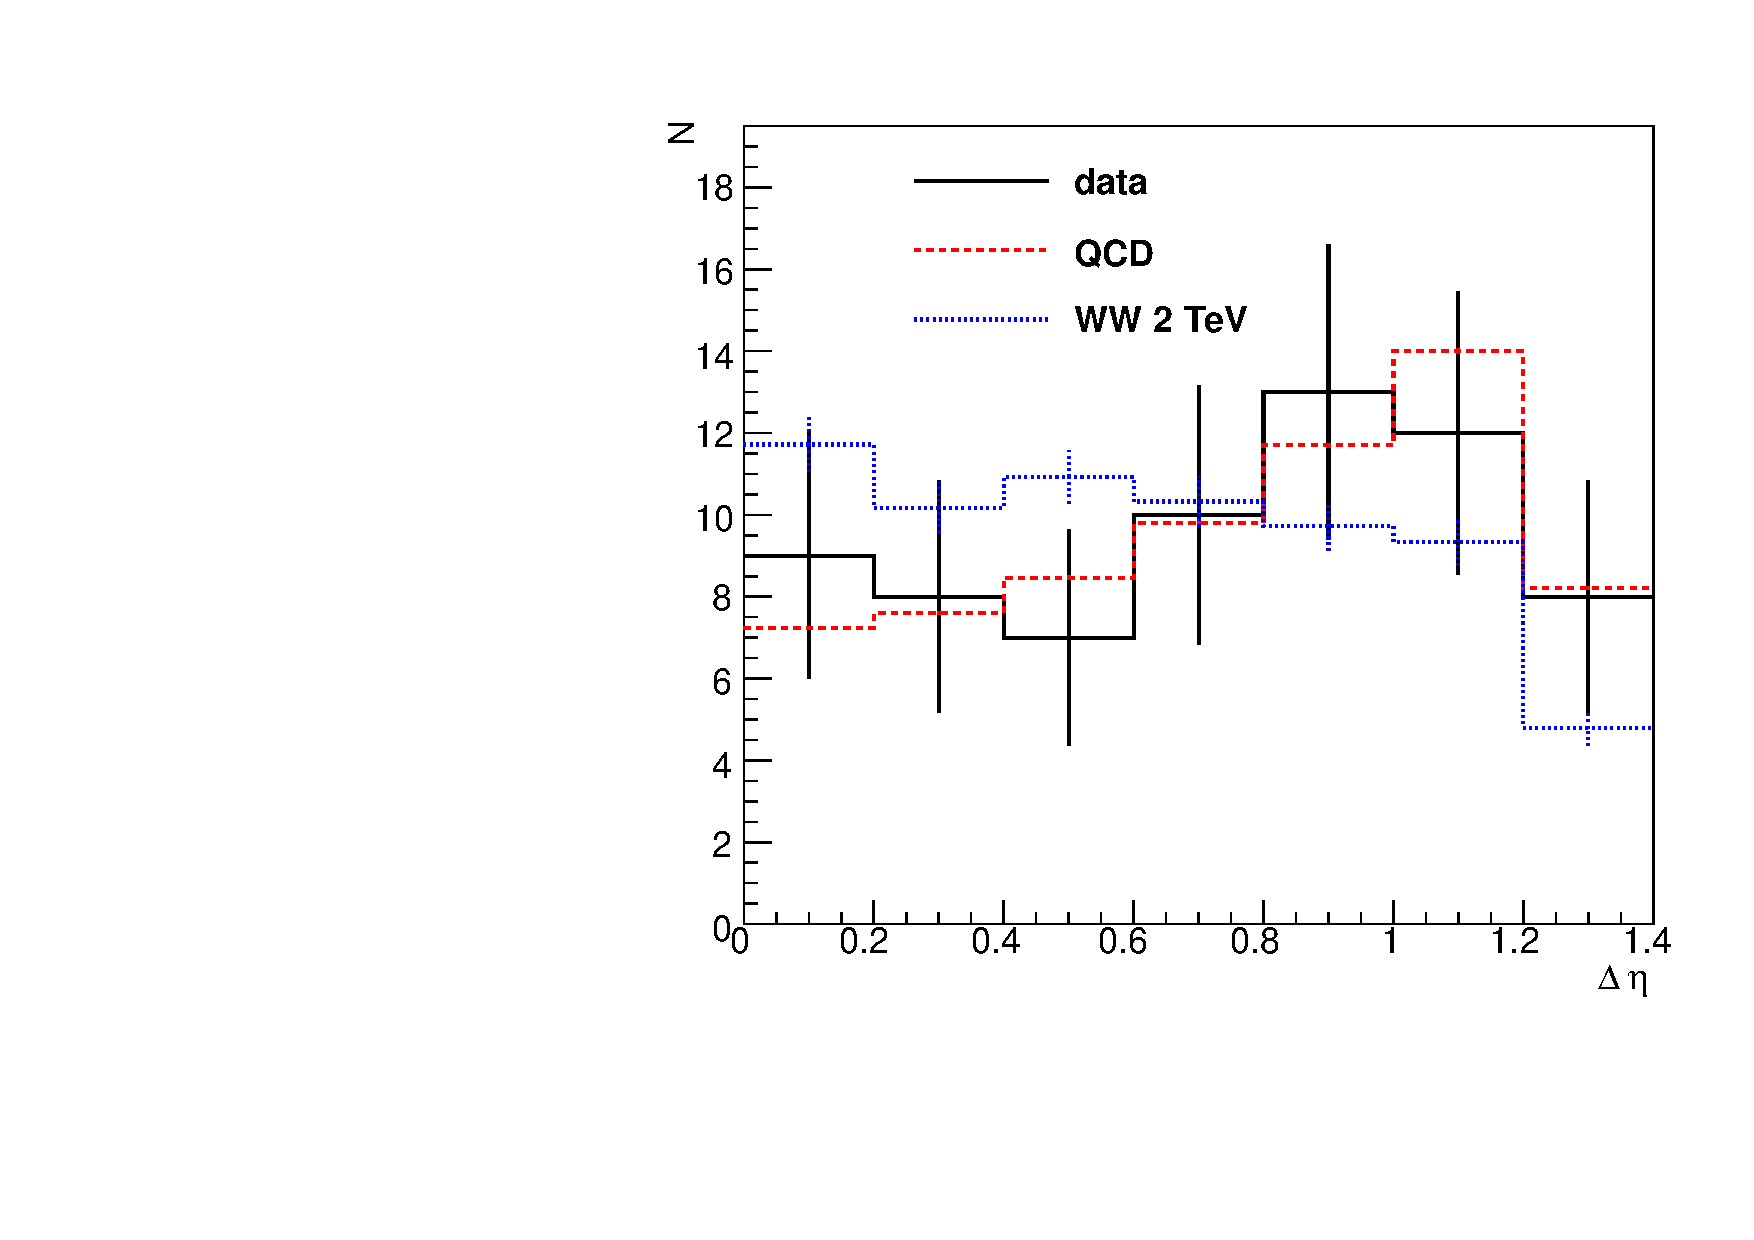
\includegraphics[width=0.48\textwidth,angle=0]{EXO-12-024/figs/appendix/data2012_v3_deta_2mtag_2mdtag_0mtag_deta.pdf}
%\end{center}
%\caption{Difference of the pseudo-rapidities of the two leading jets for events with dijet mass larger than 1.6~TeV, 
%comparing data, Madgraph+Pythia6 QCD MC and Herwig++ $G_{RS}$ to WW with a mass of 2~TeV MC.
%Top-left: Data+MC are required to have 2-tags. Top-right: Data+MC are required to 0-tags.
%Bottom: Data are required to have 2-tags, MC are required to have 0-tags.}
%\label{fig:app}
%\end{figure}

%\begin{figure}[htb]
%\begin{center}
%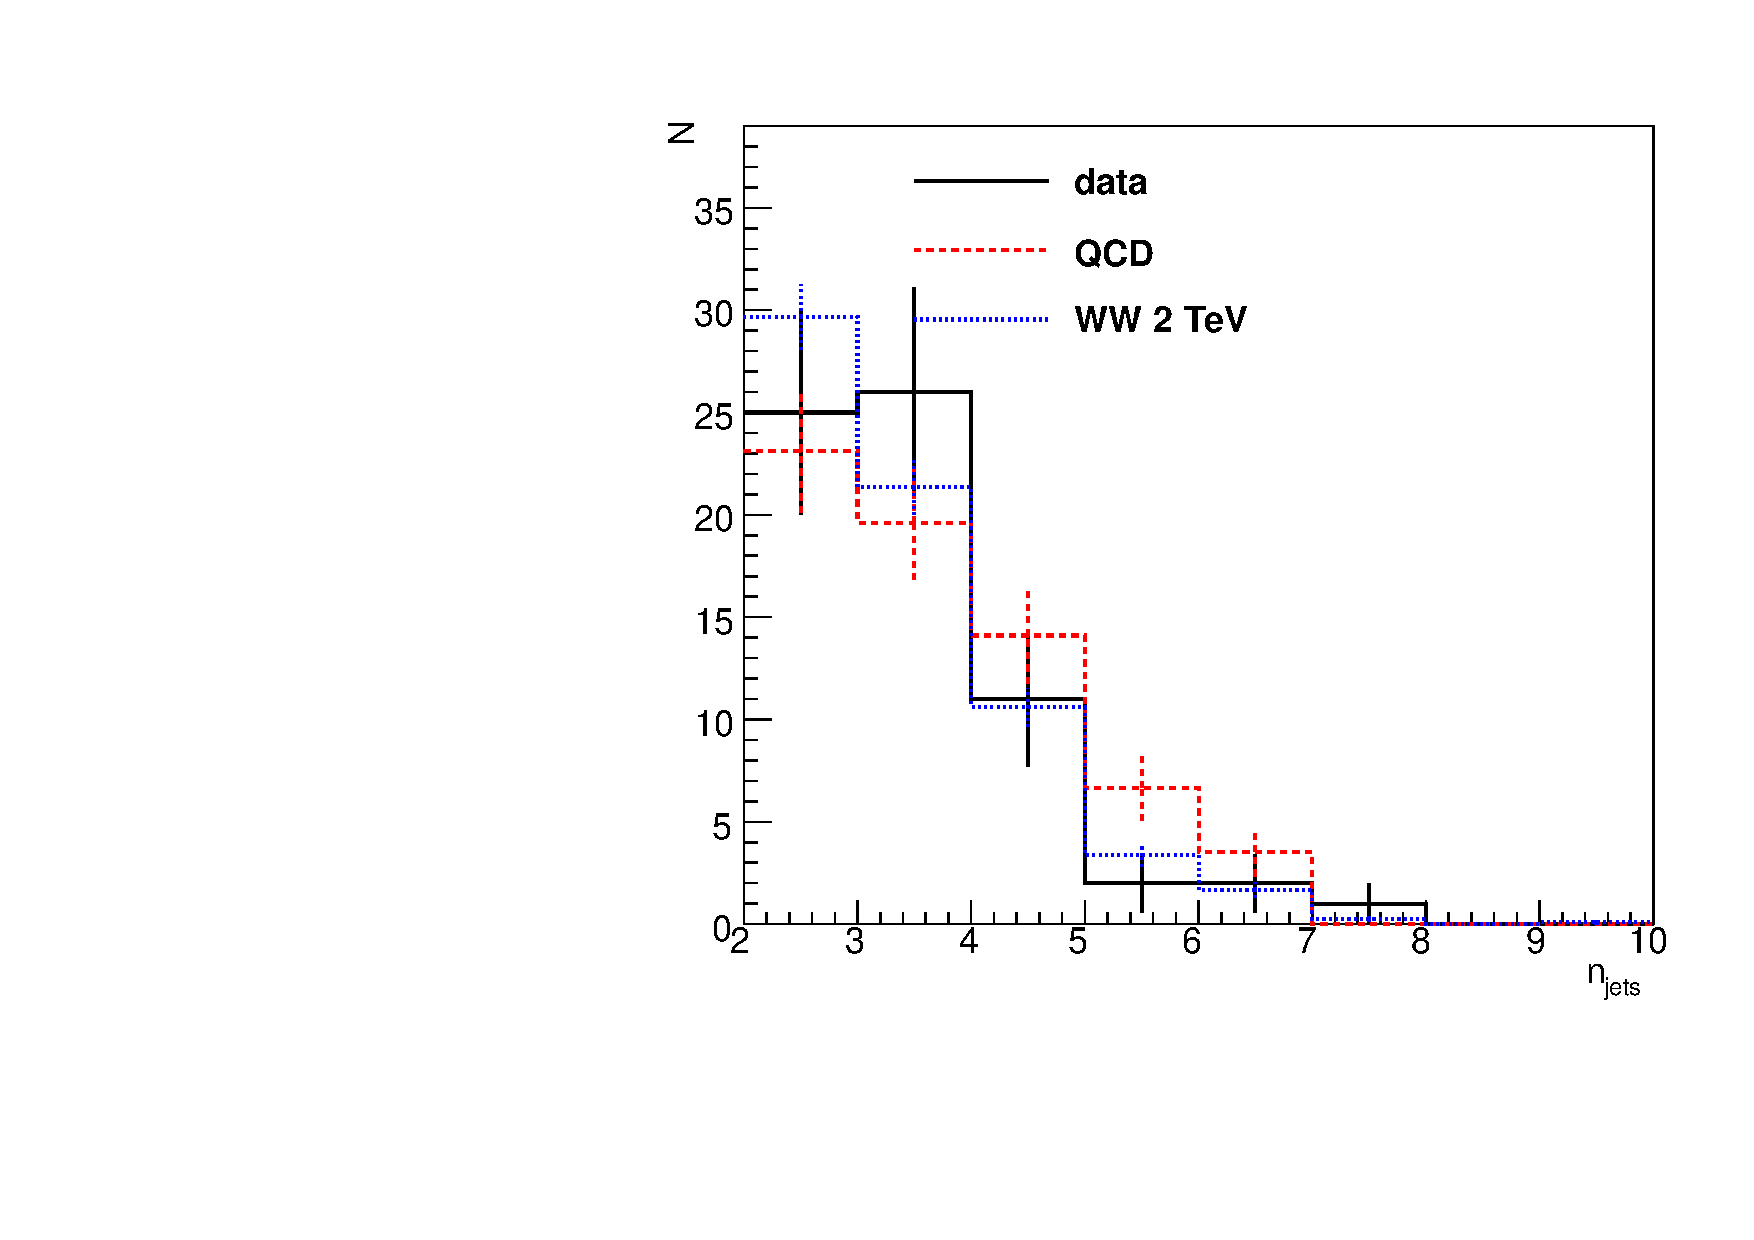
\includegraphics[width=0.48\textwidth,angle=0]{EXO-12-024/figs/appendix/data2012_v2_njets_2mtag_2mdtag_njets.pdf}
%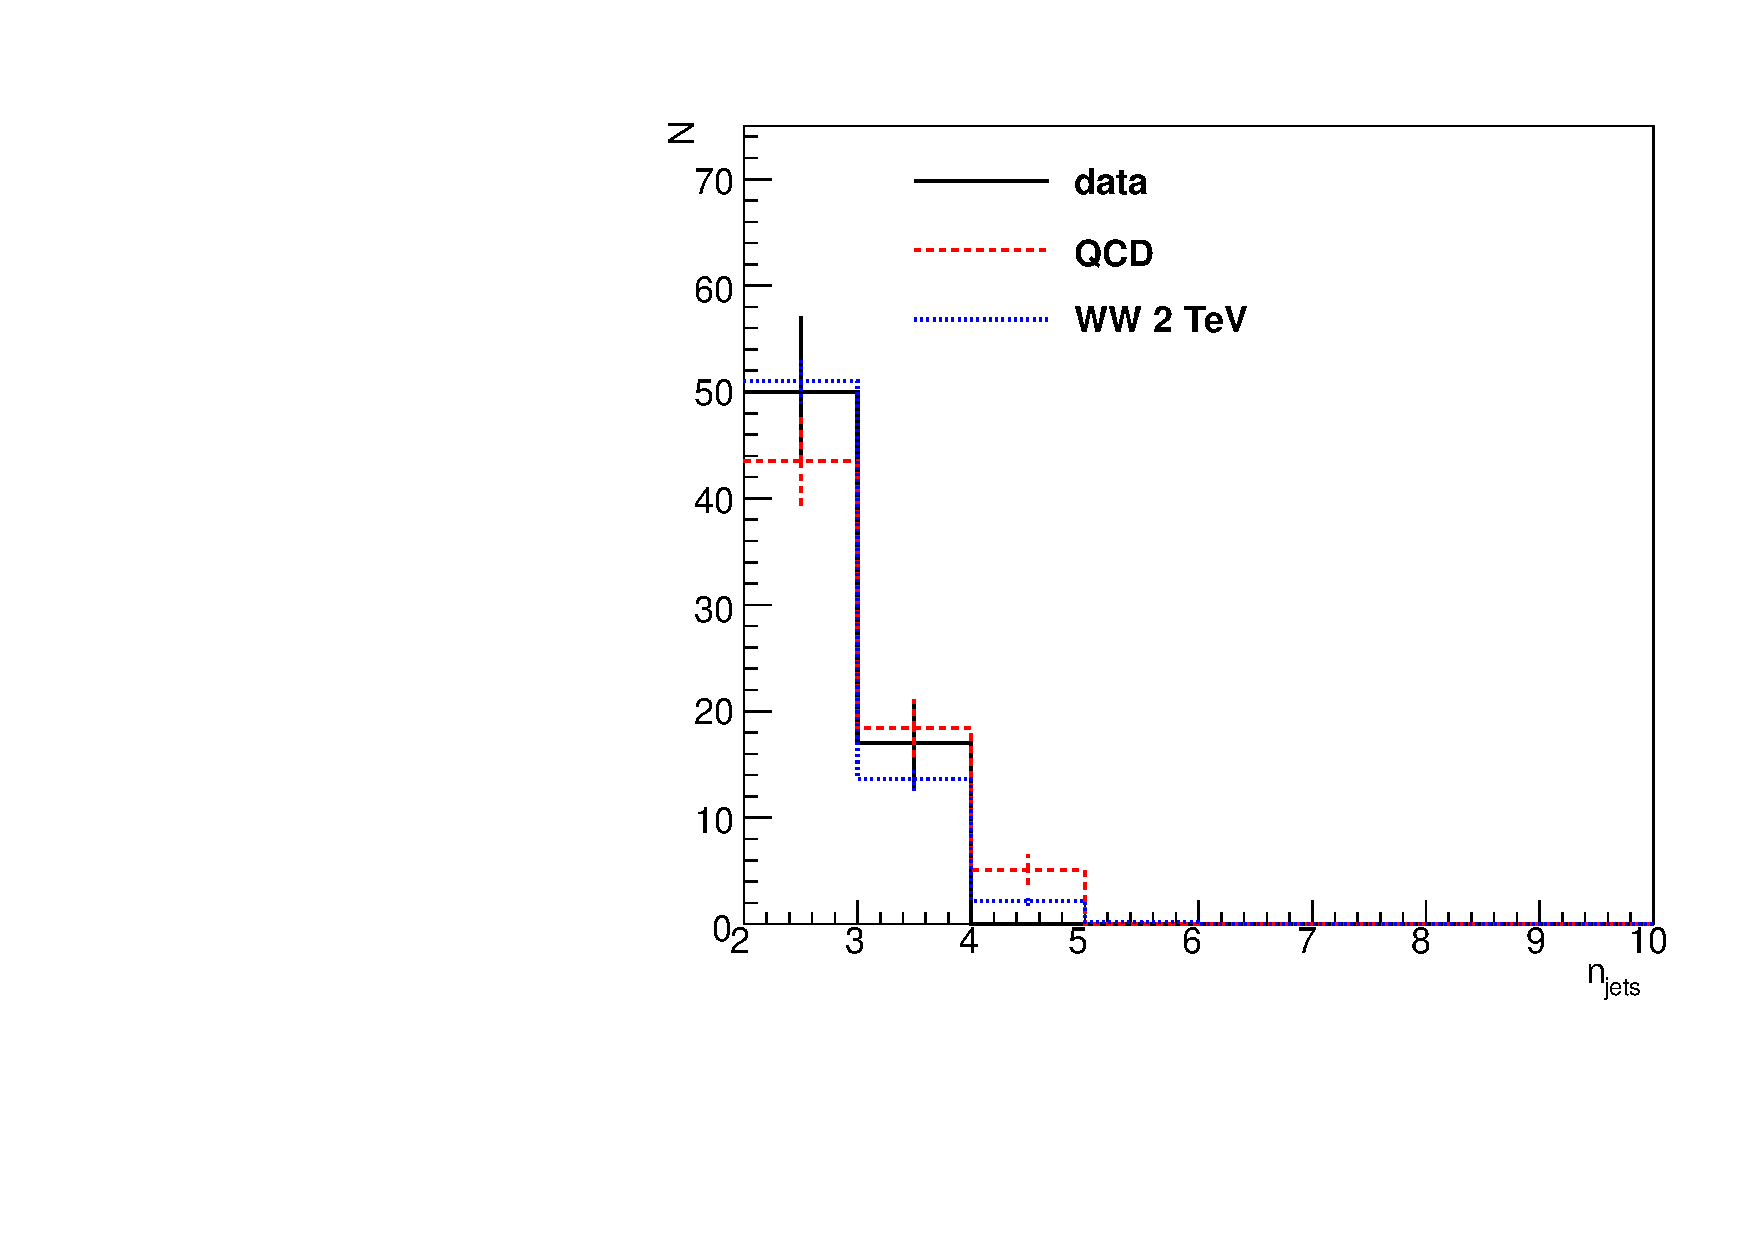
\includegraphics[width=0.48\textwidth,angle=0]{EXO-12-024/figs/appendix/data2012_v3_njetsCA8_2mtag_2mdtag_njetsCA8.pdf}
%\end{center}
%\caption{Comparison of data, Madgraph+Pythia6 QCD MC and Herwig++ $G_{RS}$ to WW with a mass of 2~TeV MC
%for events with dijet mass larger than 1.6~TeV.
%Left: Number of reconstructed AK5 jets with $p_T>30$~GeV.
%Right: Number of reconstructed pruned CA8 jets with $p_T>100$~GeV.}
%\label{fig:app}
%\end{figure}

%\clearpage
%\subsection{limits for other six categories}
%To investigate the bump at 2.0 \TeVcc, we perform the tests on other six categories 
%to get limits. 
%
%\begin{itemize}
%\item (a) neither of the two leading jets passes the jet mass cut($ [70 GeV, 100 GeV]$) 
%\item (b) only one of the two leading jets passes the jet mass cut, but neither passes the massdrop cut
%\item (c) only one jet passes the jet mass cut and massdrop cut
%\item (d) two leading jets pass the jet mass cut, both fail the massdrop cut
%\item (d) two leading jets pass the jet mass cut, but one fails the massdrop cut
%\item (e) two leading jets pass all the cuts  
%\end{itemize}
%
%
%\begin{figure}[htb]
%\begin{center}
%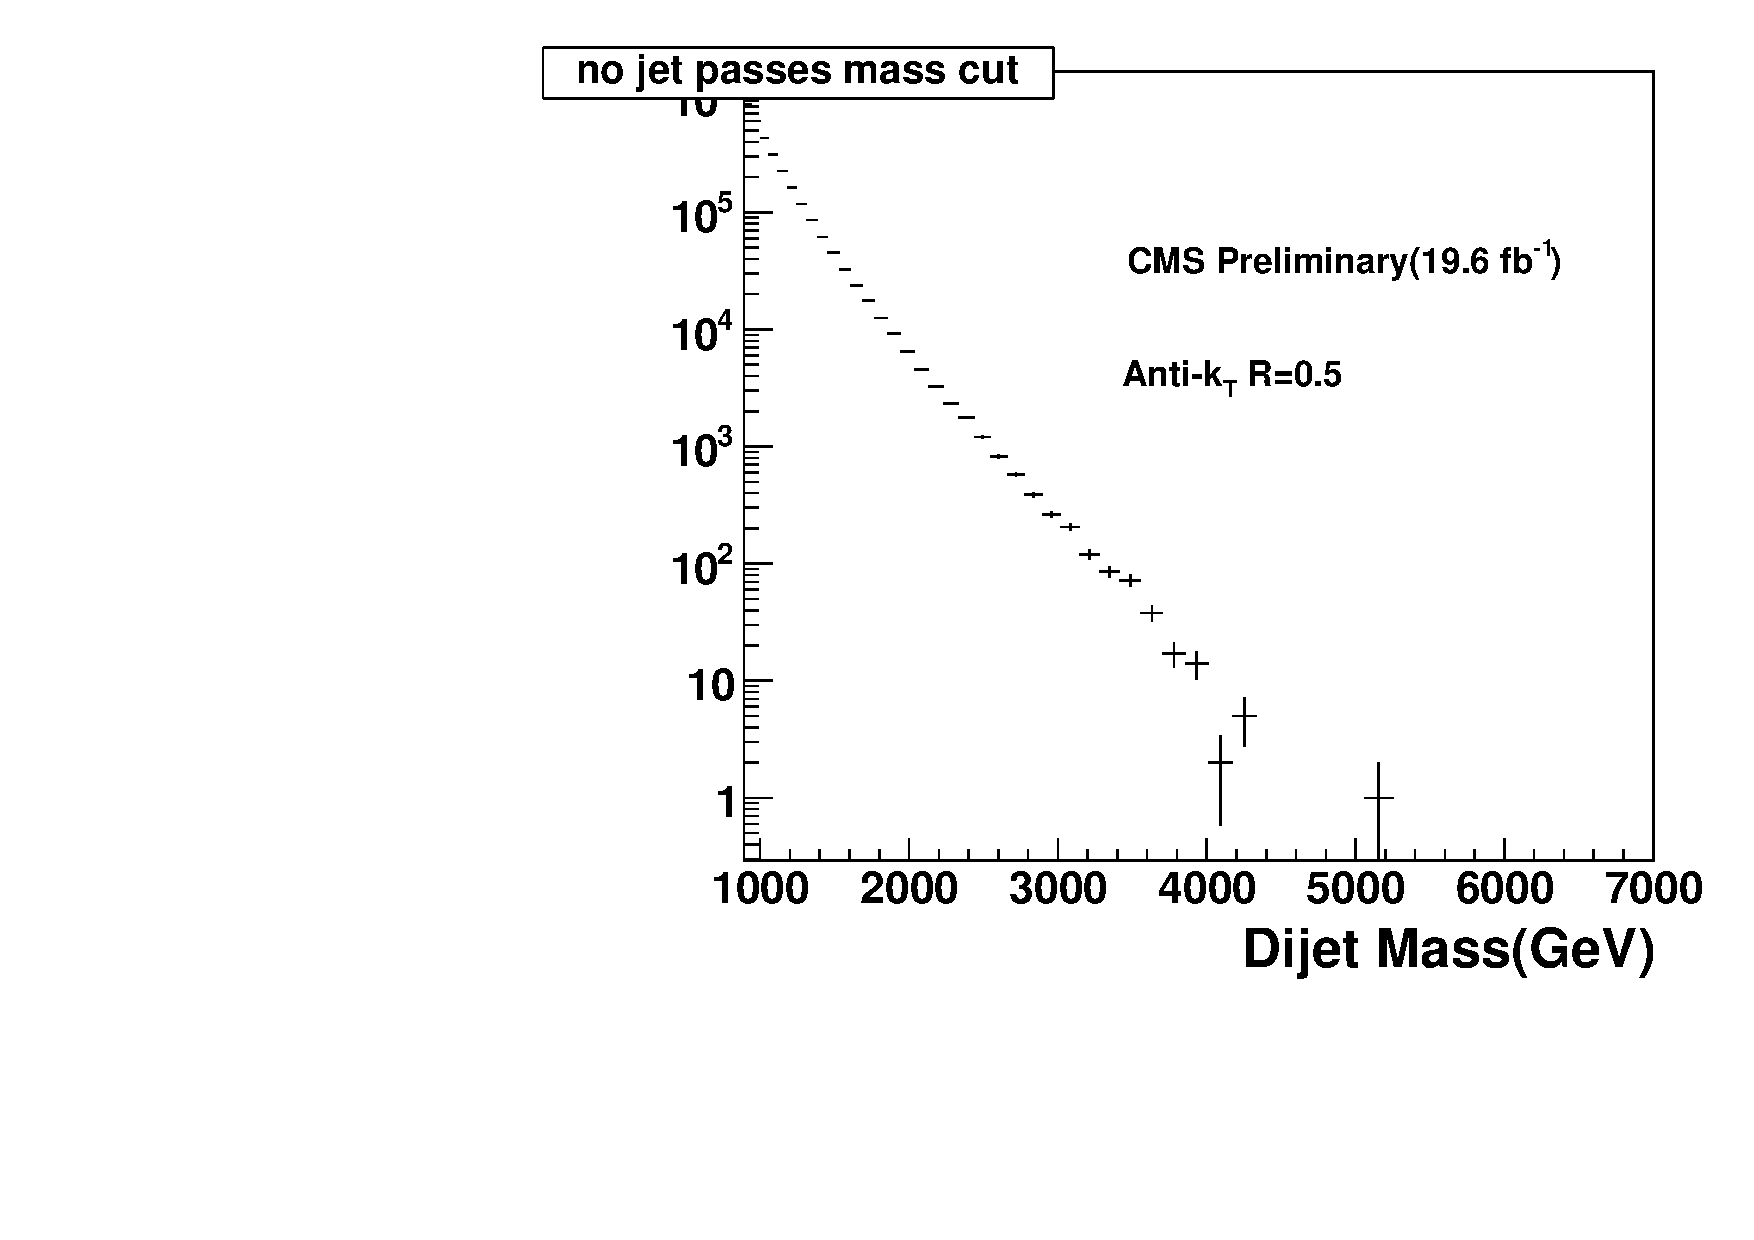
\includegraphics[width=0.48\textwidth,angle=0]{EXO-12-024/figs/VVCheck/noMassrebin.pdf}
%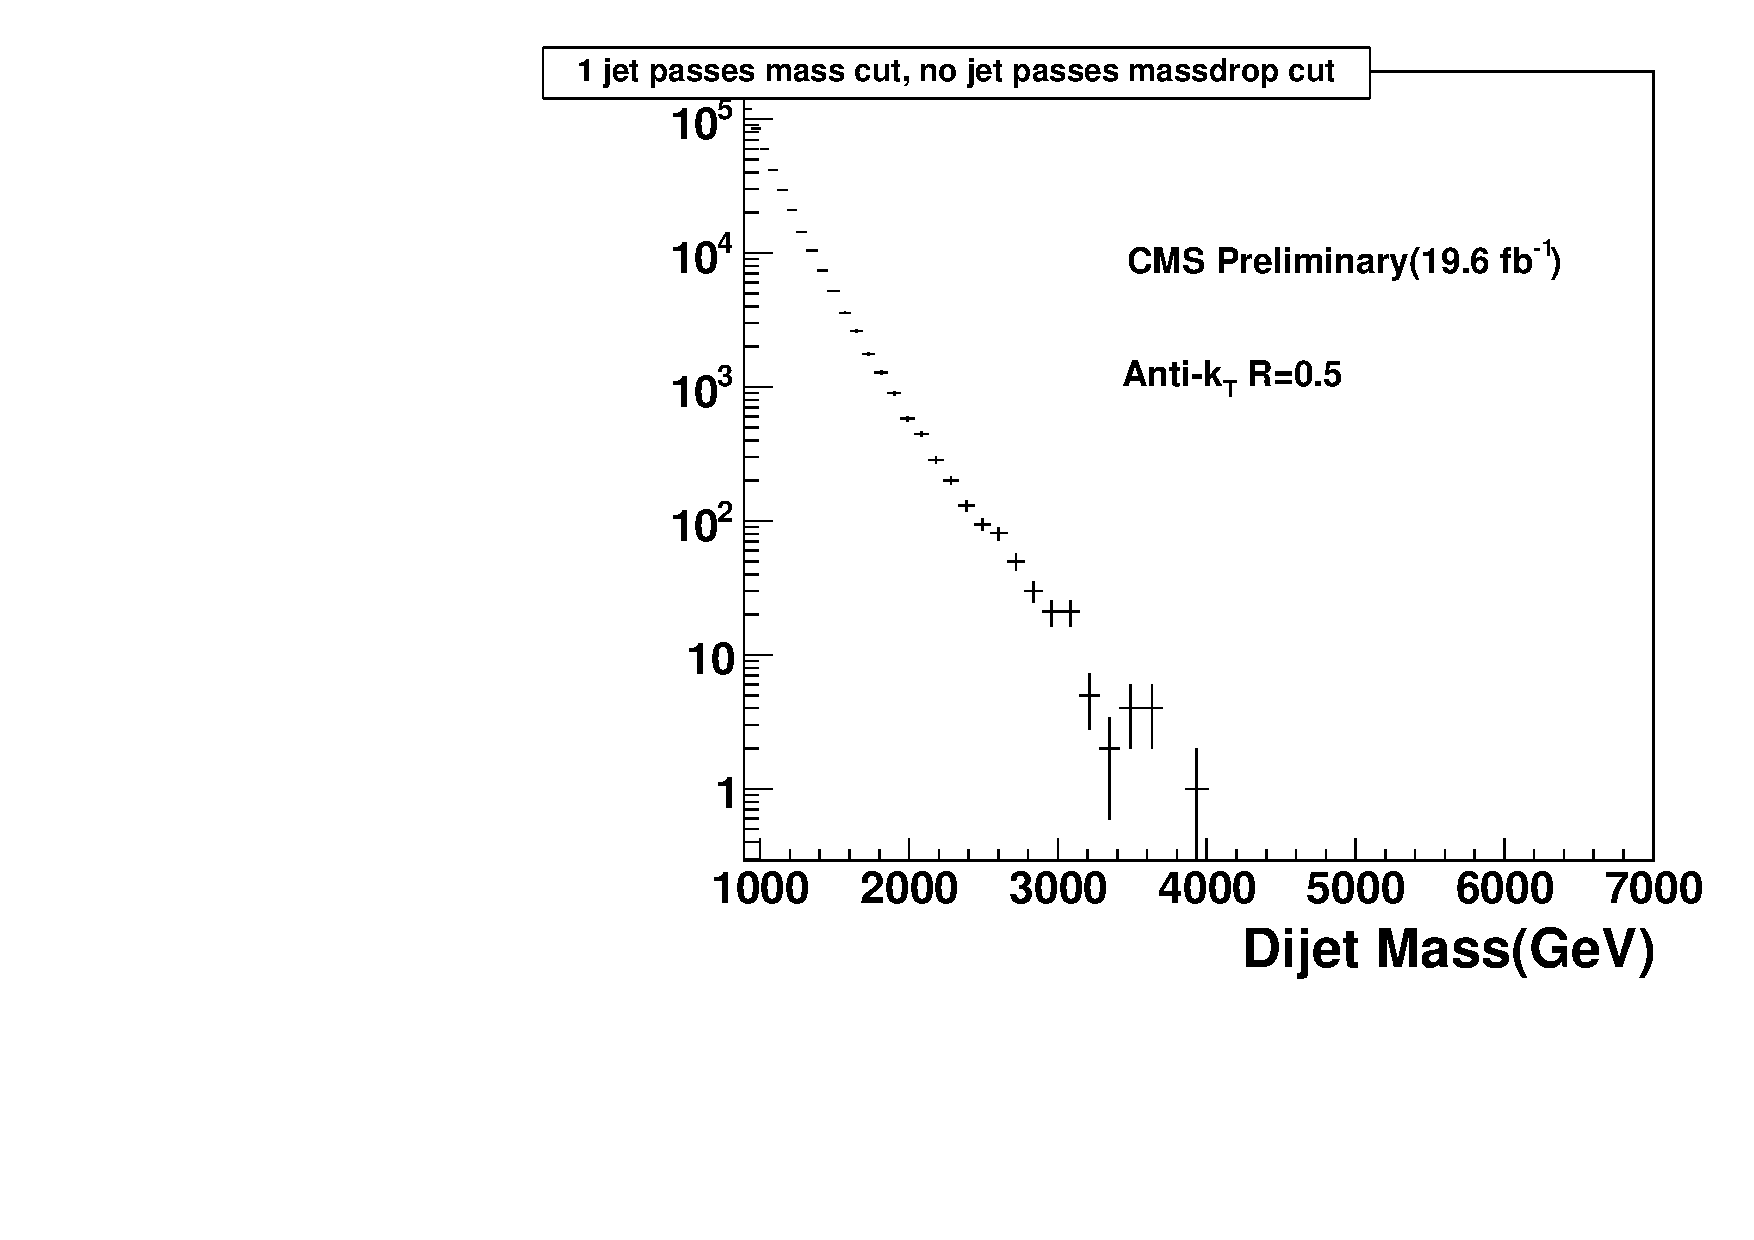
\includegraphics[width=0.48\textwidth,angle=0]{EXO-12-024/figs/VVCheck/singleMassNoDroprebin.pdf}
%\end{center}
%\caption{Dijet mass distribution}
%\label{fig:ab}
%\end{figure}
%
%\begin{figure}[htb]
%\begin{center}
%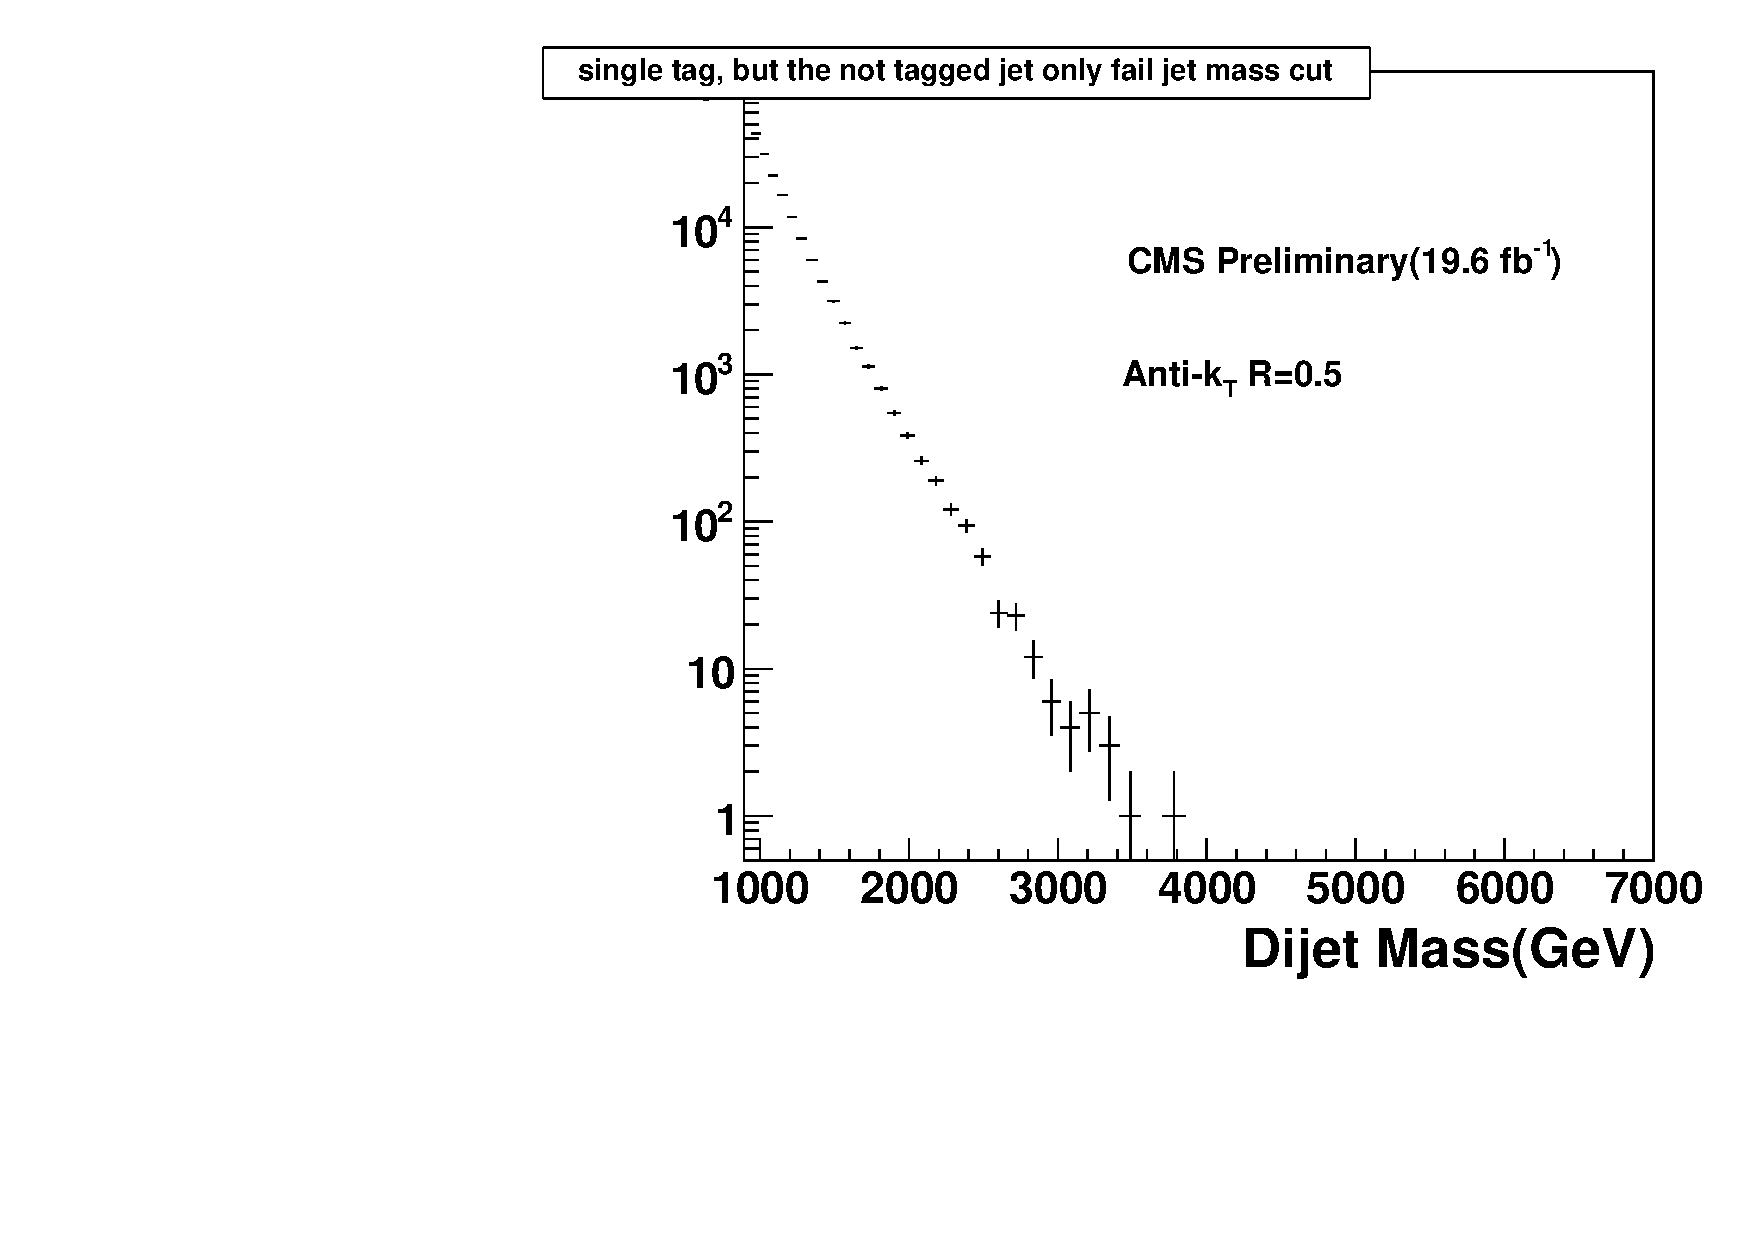
\includegraphics[width=0.48\textwidth,angle=0]{EXO-12-024/figs/VVCheck/singleTagExclusiverebin.pdf}
%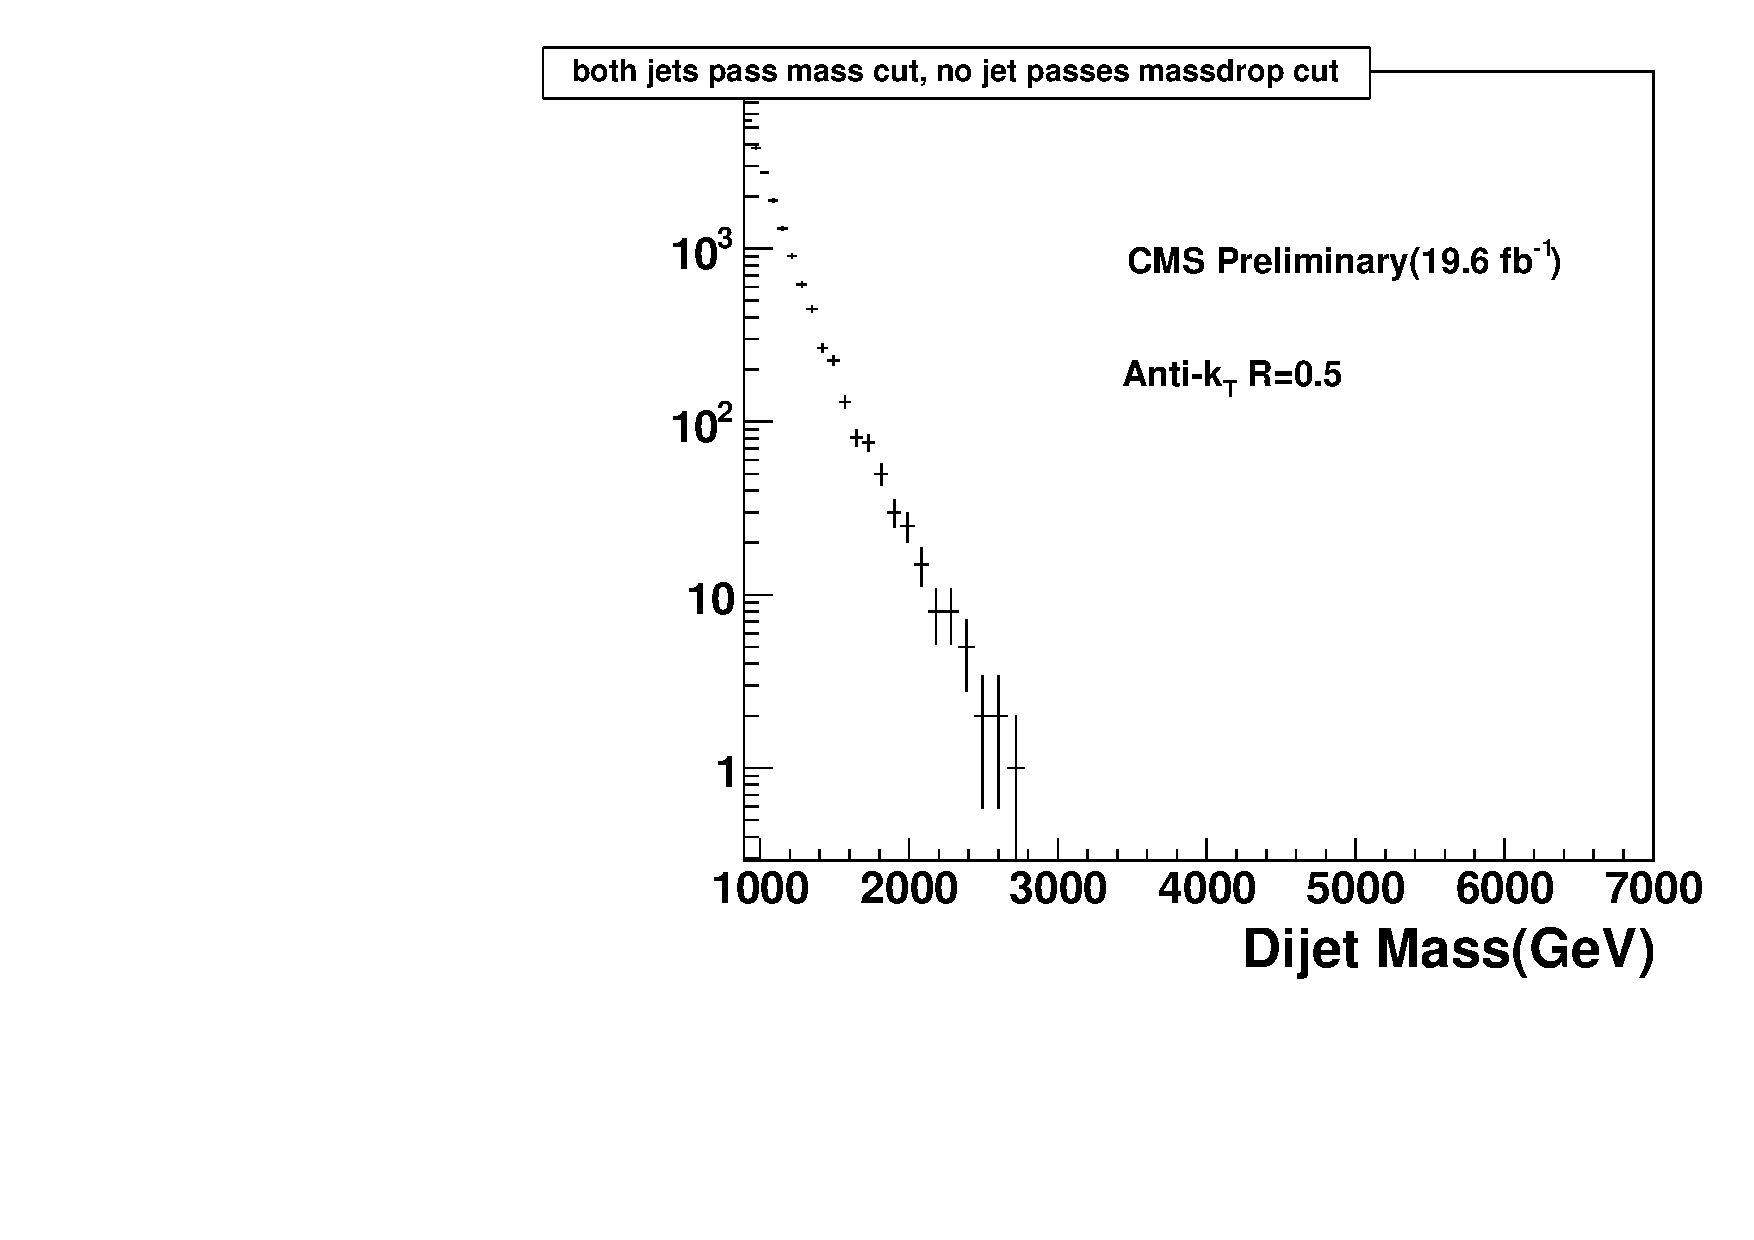
\includegraphics[width=0.48\textwidth,angle=0]{EXO-12-024/figs/VVCheck/doubleMassNoDroprebin.pdf}
%\end{center}
%\caption{Dijet mass distribution}
%\label{fig:cd}
%\end{figure}
%
%\begin{figure}[htb]
%\begin{center}
%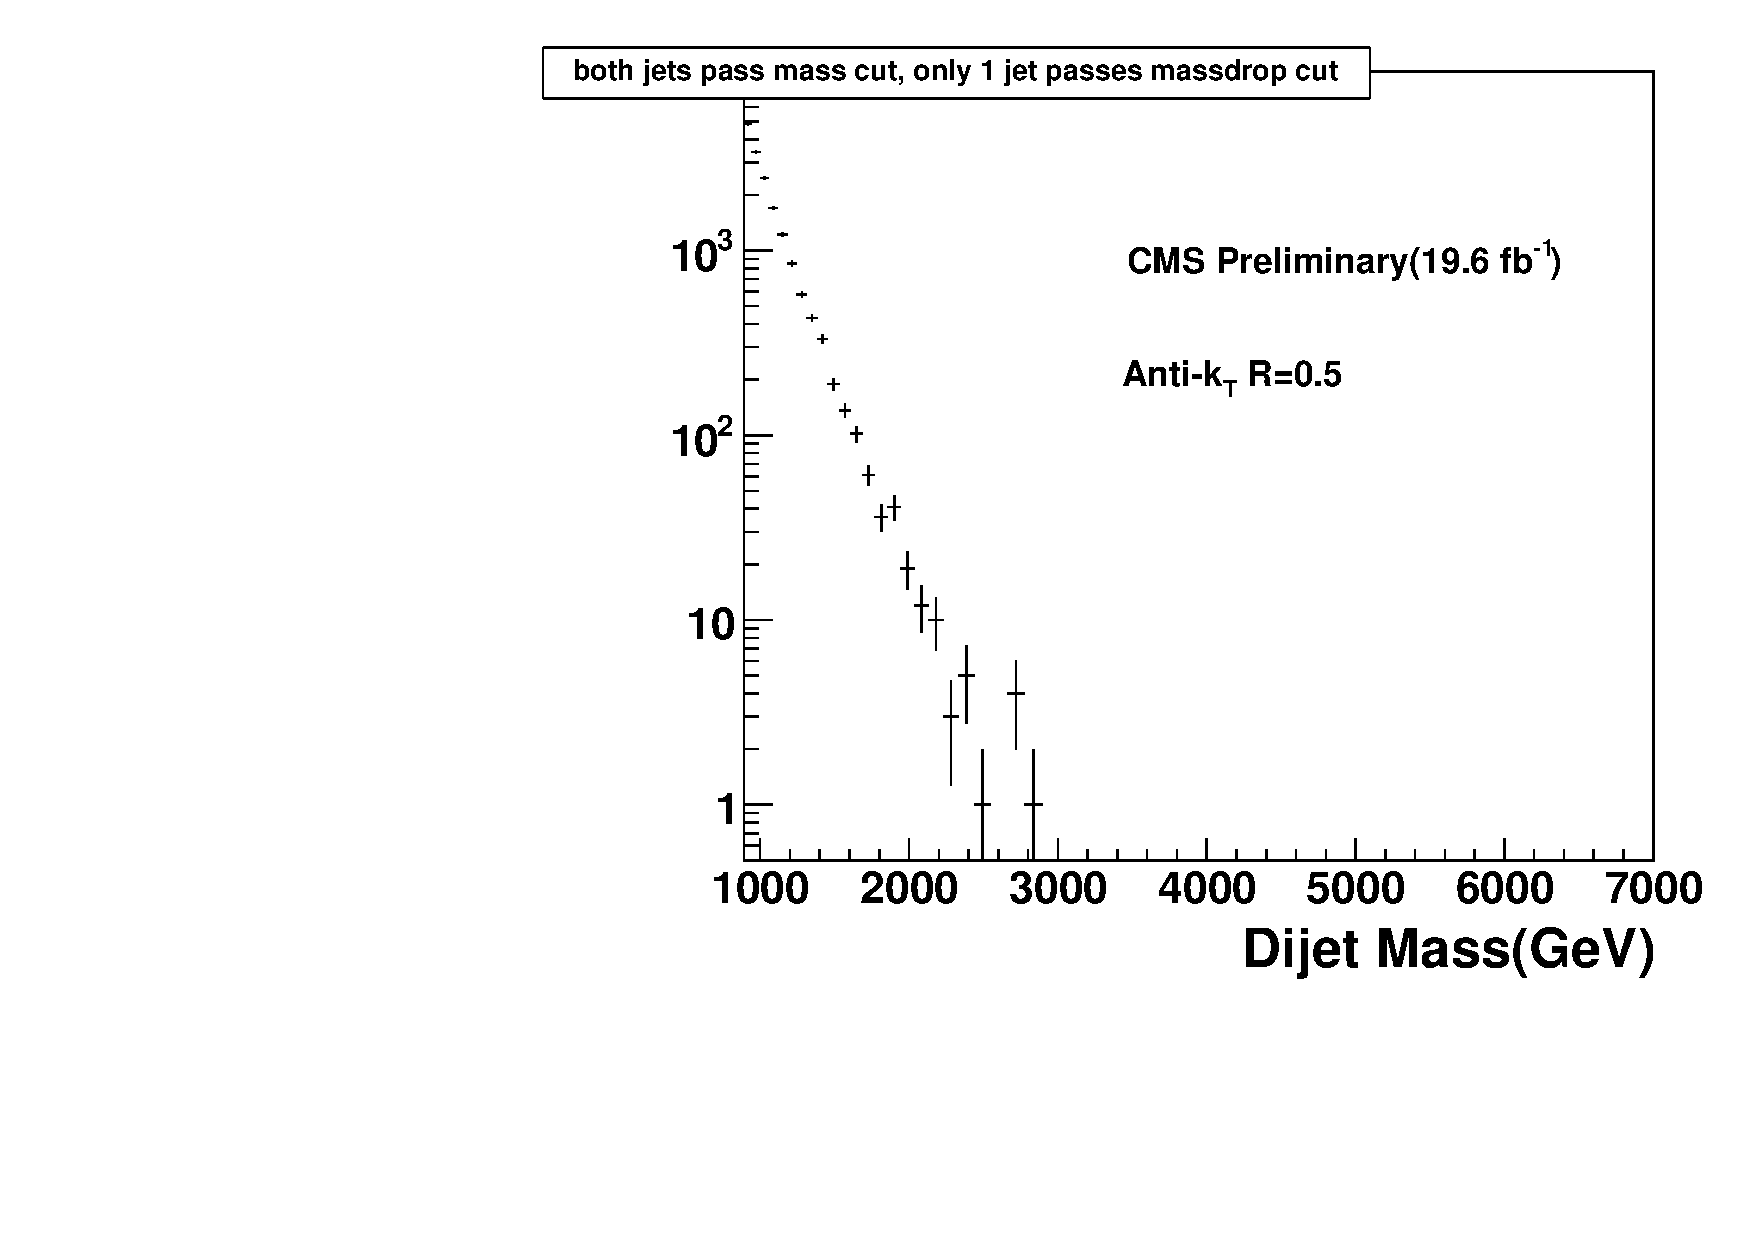
\includegraphics[width=0.48\textwidth,angle=0]{EXO-12-024/figs/VVCheck/doubleMassSingleDroprebin.pdf}
%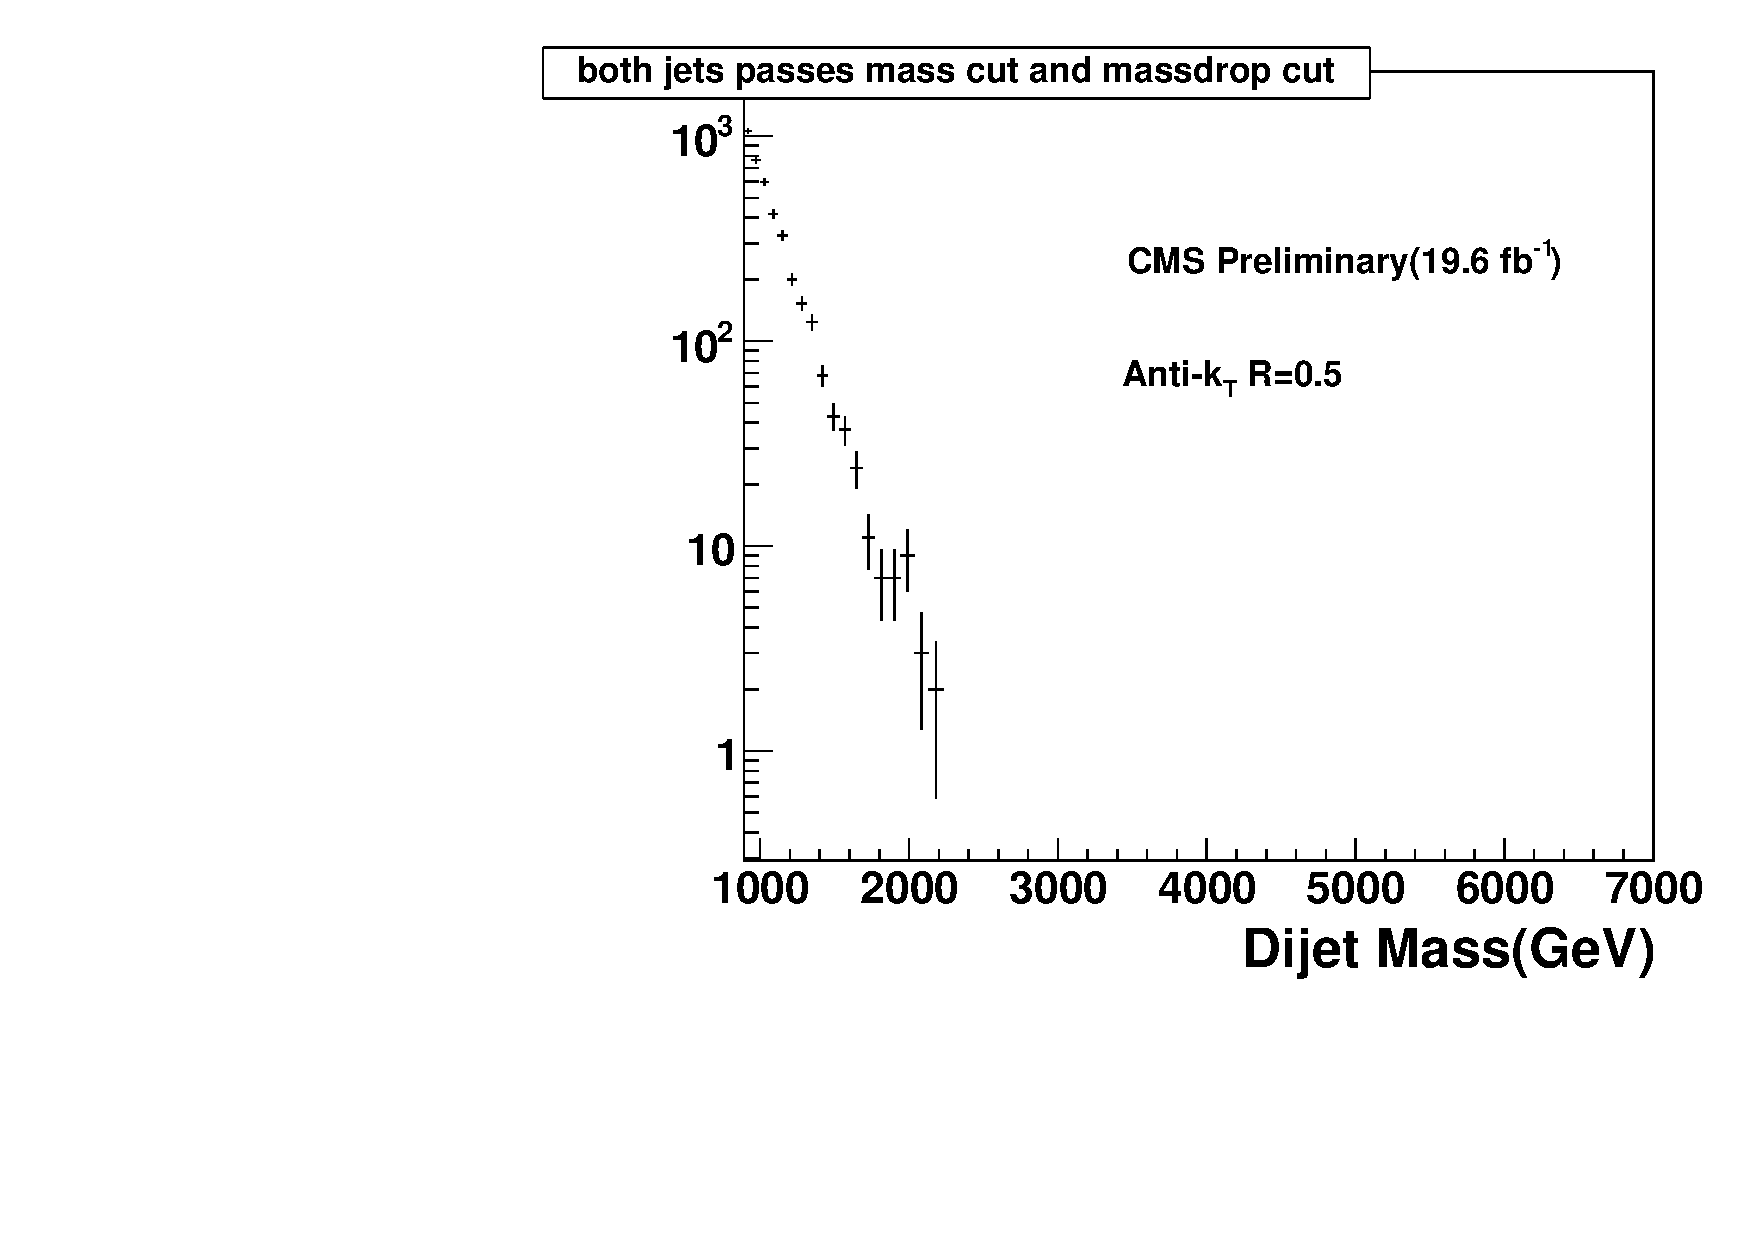
\includegraphics[width=0.48\textwidth,angle=0]{EXO-12-024/figs/VVCheck/doubleMassDoubleDroprebin.pdf}
%\end{center}
%\caption{Dijet mass distribution}
%\label{fig:ef}
%\end{figure}
%
%
%\begin{figure}[htb]
%\begin{center} 
%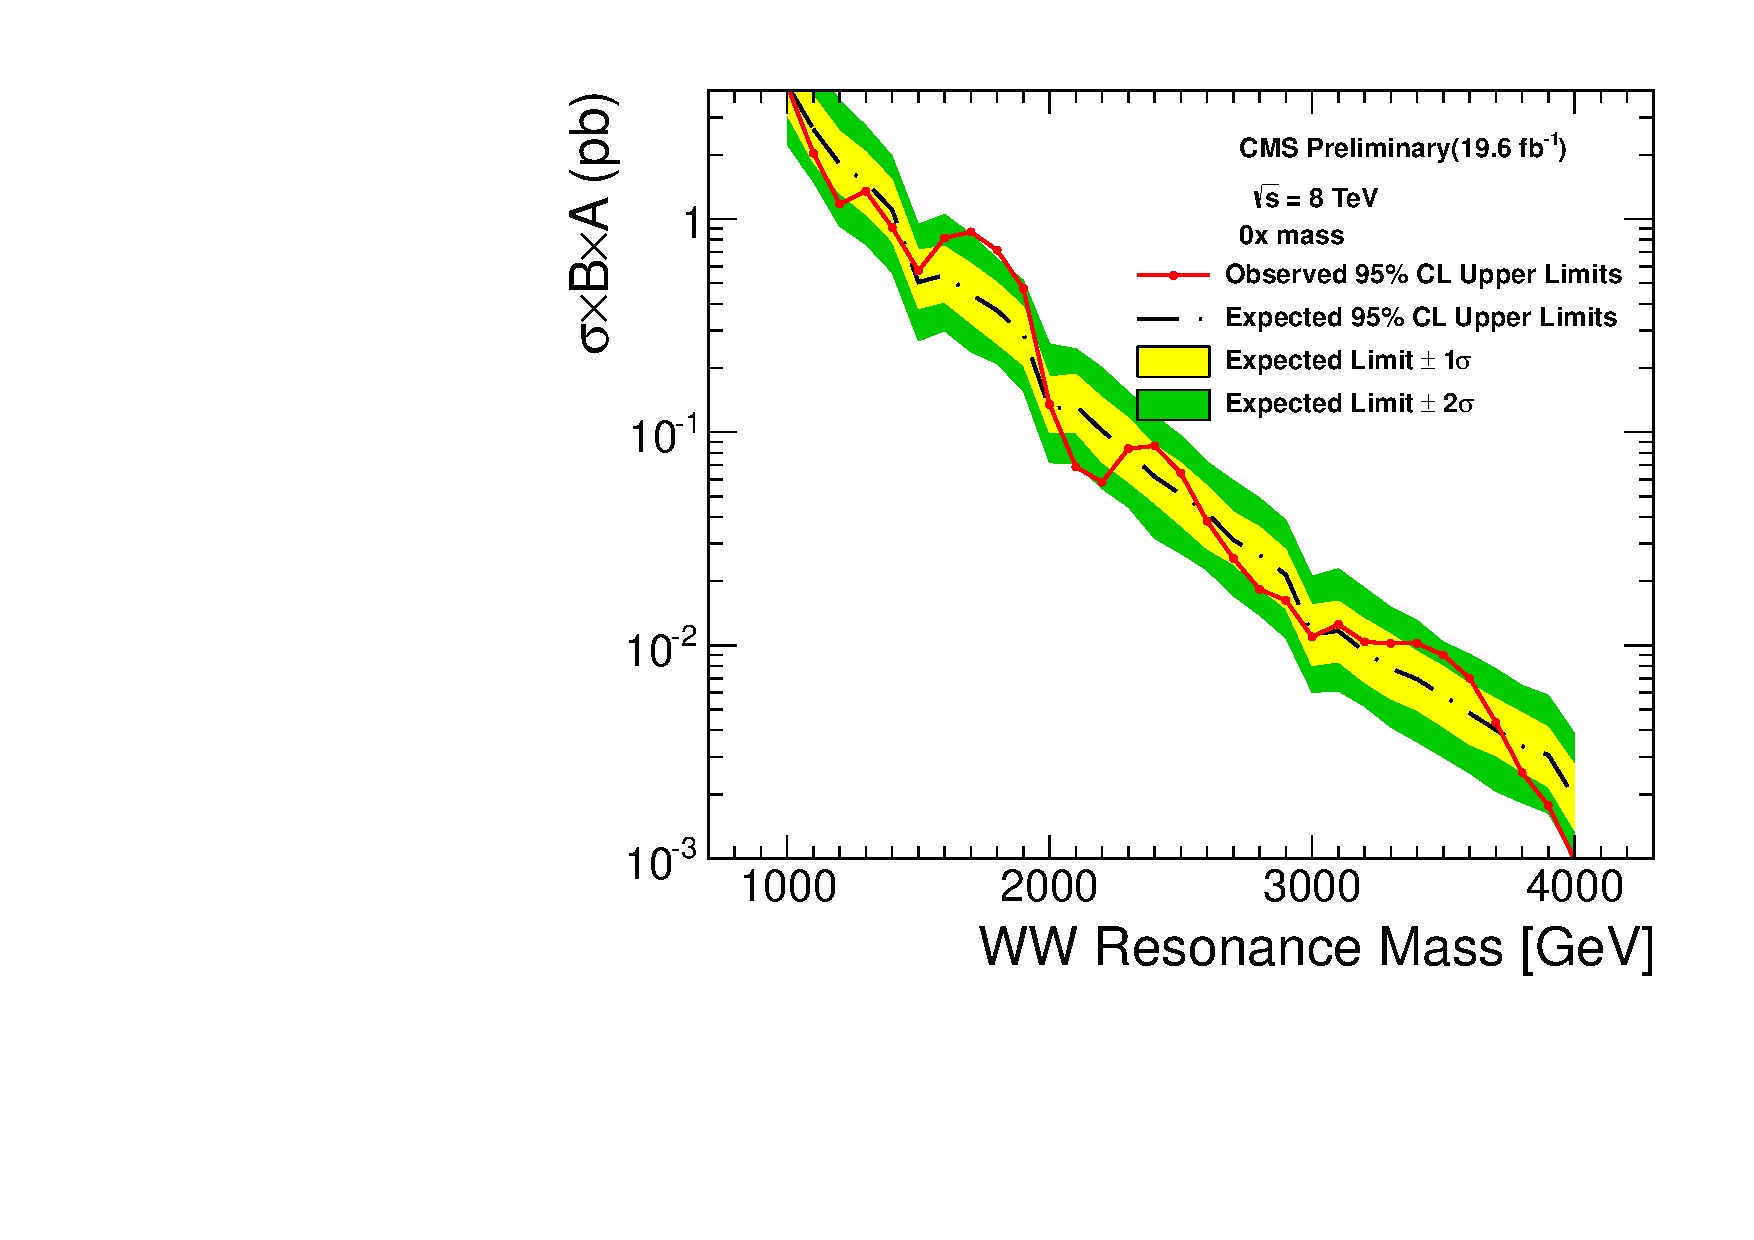
\includegraphics[width=0.48\textwidth,angle=0]{EXO-12-024/figs/VVCheck/RSGWWherwig_0xMass_limit_obsexp.pdf}
%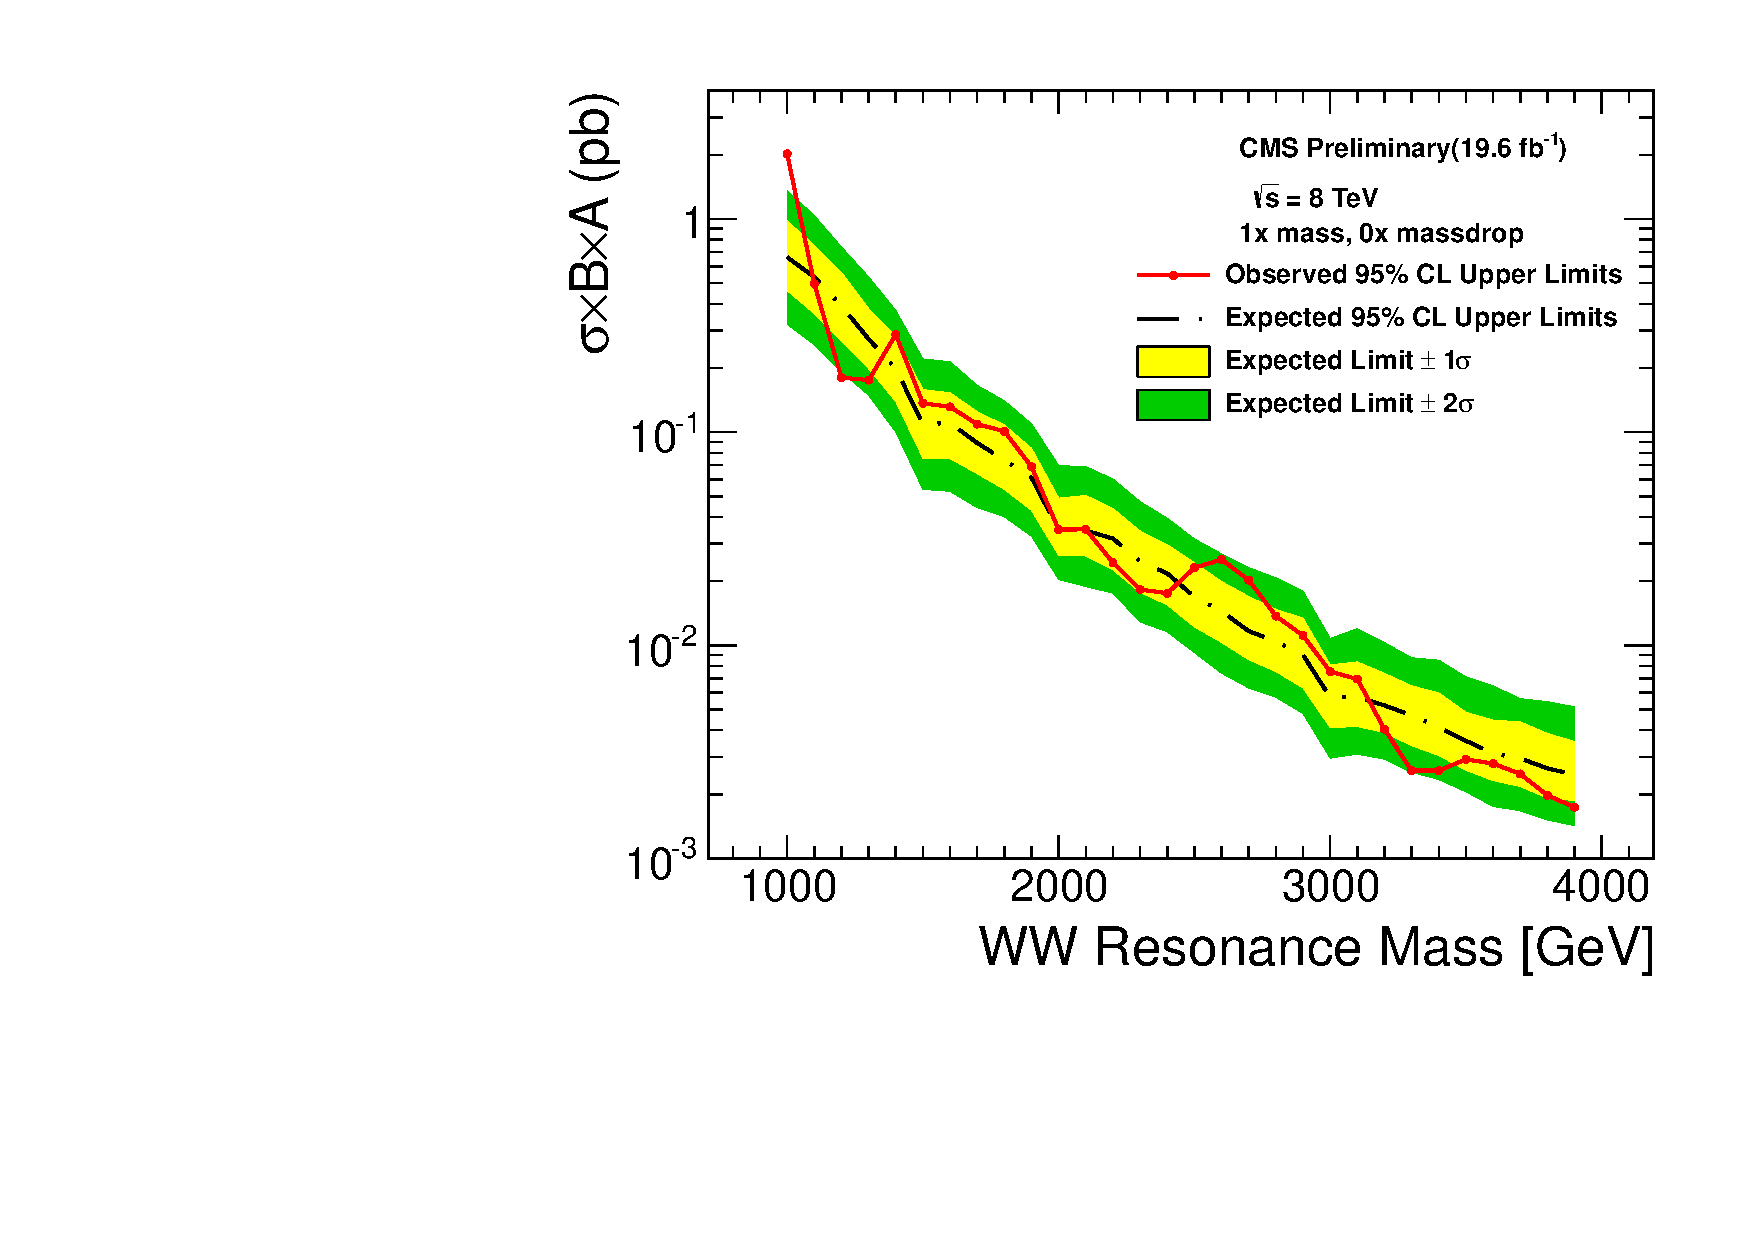
\includegraphics[width=0.48\textwidth,angle=0]{EXO-12-024/figs/VVCheck/RSGWWherwig_1xMass0xMassdrop_limit_obsexp.pdf}
%\end{center}
%\caption{limits for categories a and b}
%\label{fig:ablimit} 
%\end{figure}
%
%
%\begin{figure}[htb]
%\begin{center} 
%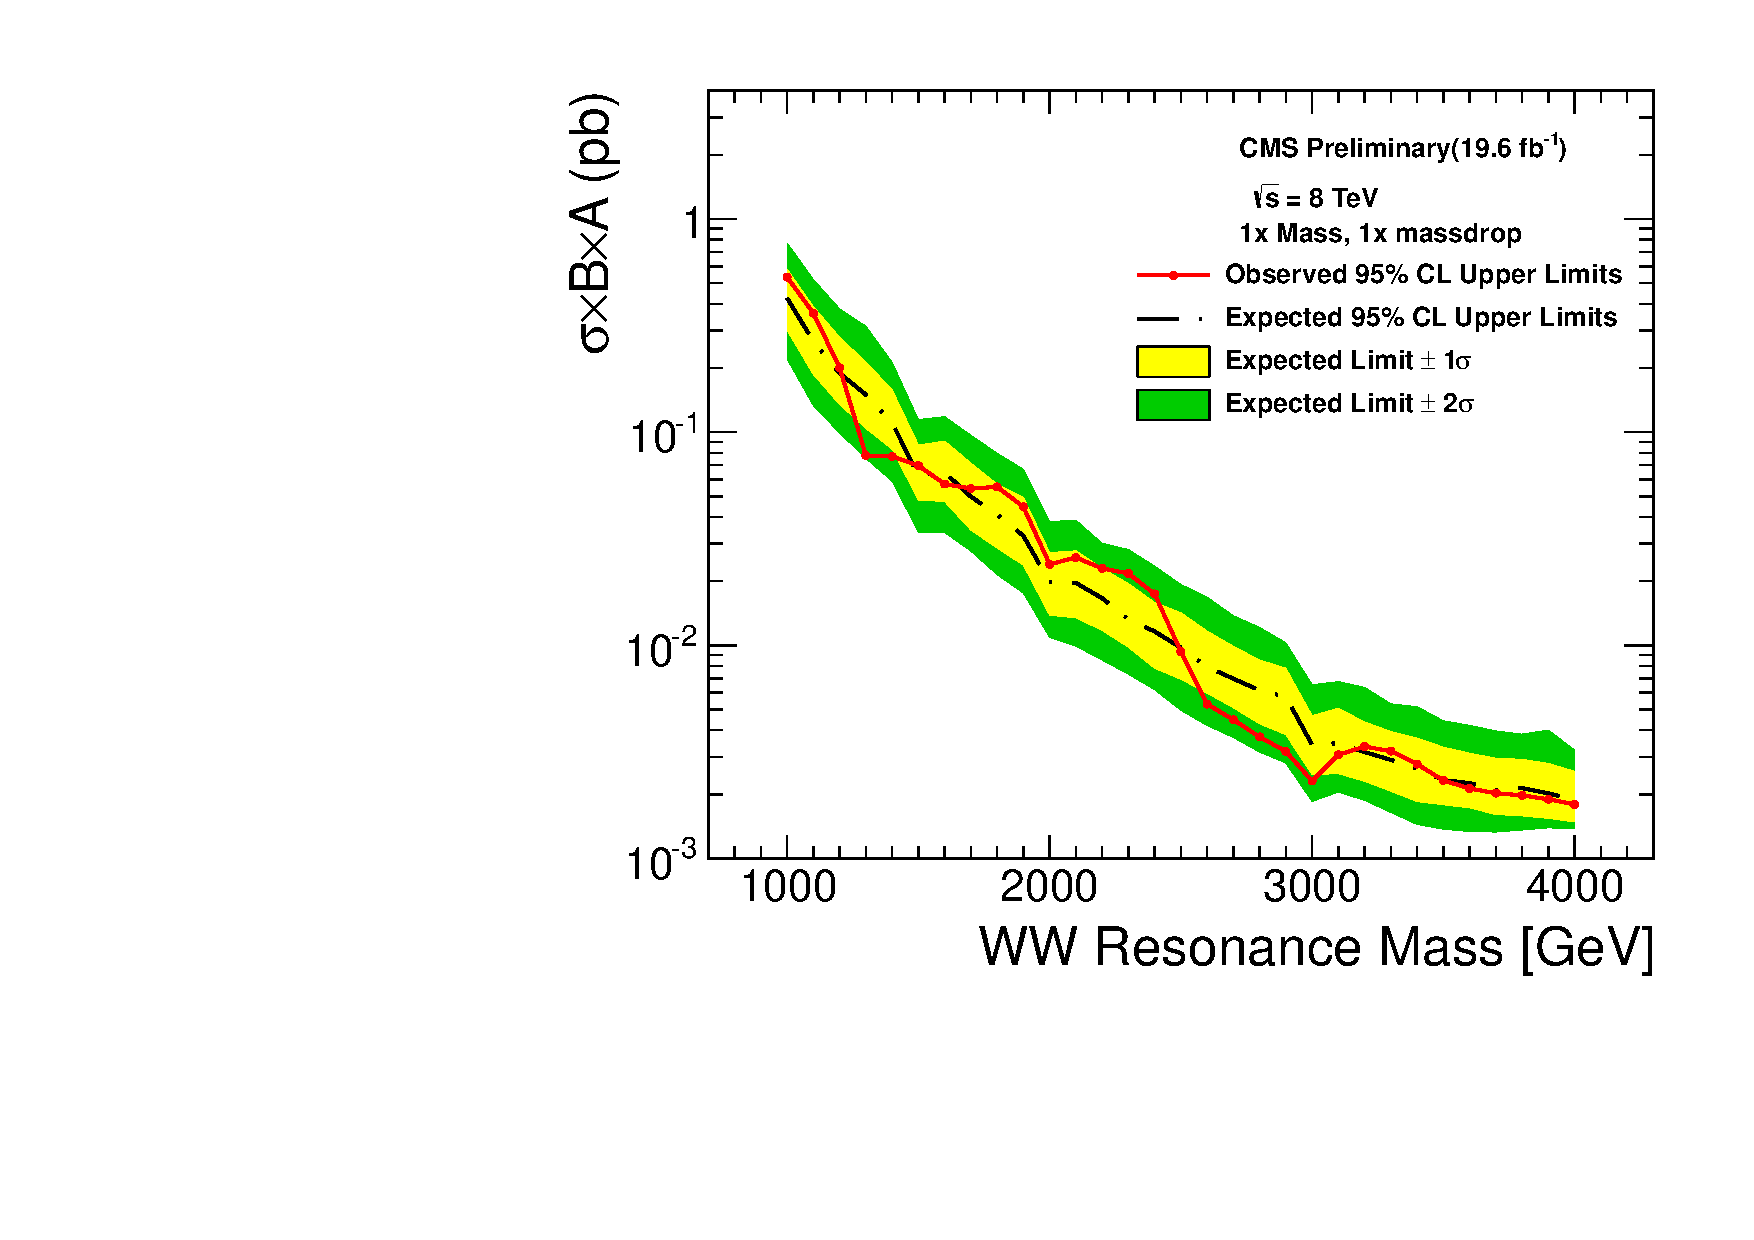
\includegraphics[width=0.48\textwidth,angle=0]{EXO-12-024/figs/VVCheck/RSGWWherwig_1xMass1xMassdrop_limit_obsexp.pdf}
%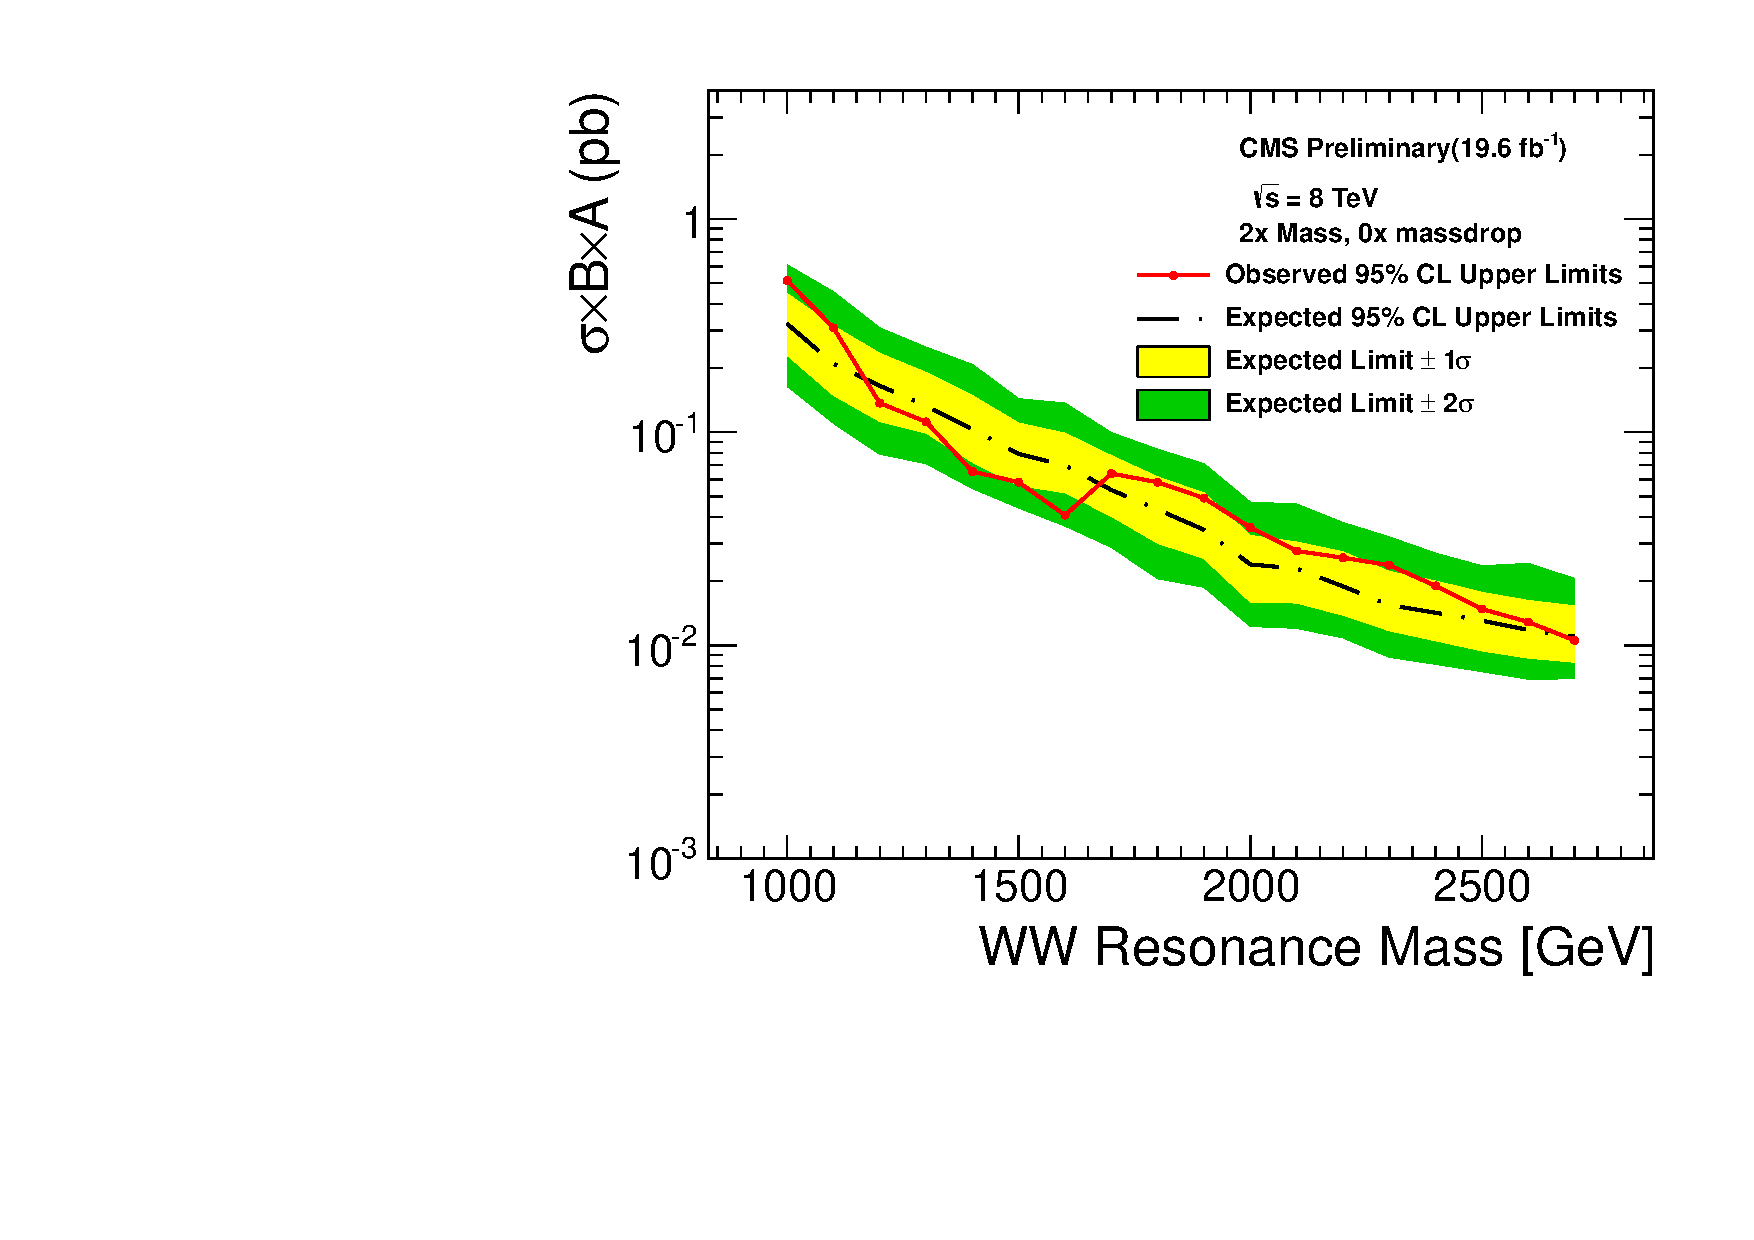
\includegraphics[width=0.48\textwidth,angle=0]{EXO-12-024/figs/VVCheck/RSGWWherwig_2xMass0xMassdrop_limit_obsexp.pdf}
%\end{center}
%\caption{limits for categories c and d}
%\label{fig:cdlimit} 
%\end{figure}
%
%\begin{figure}[htb]
%\begin{center}
%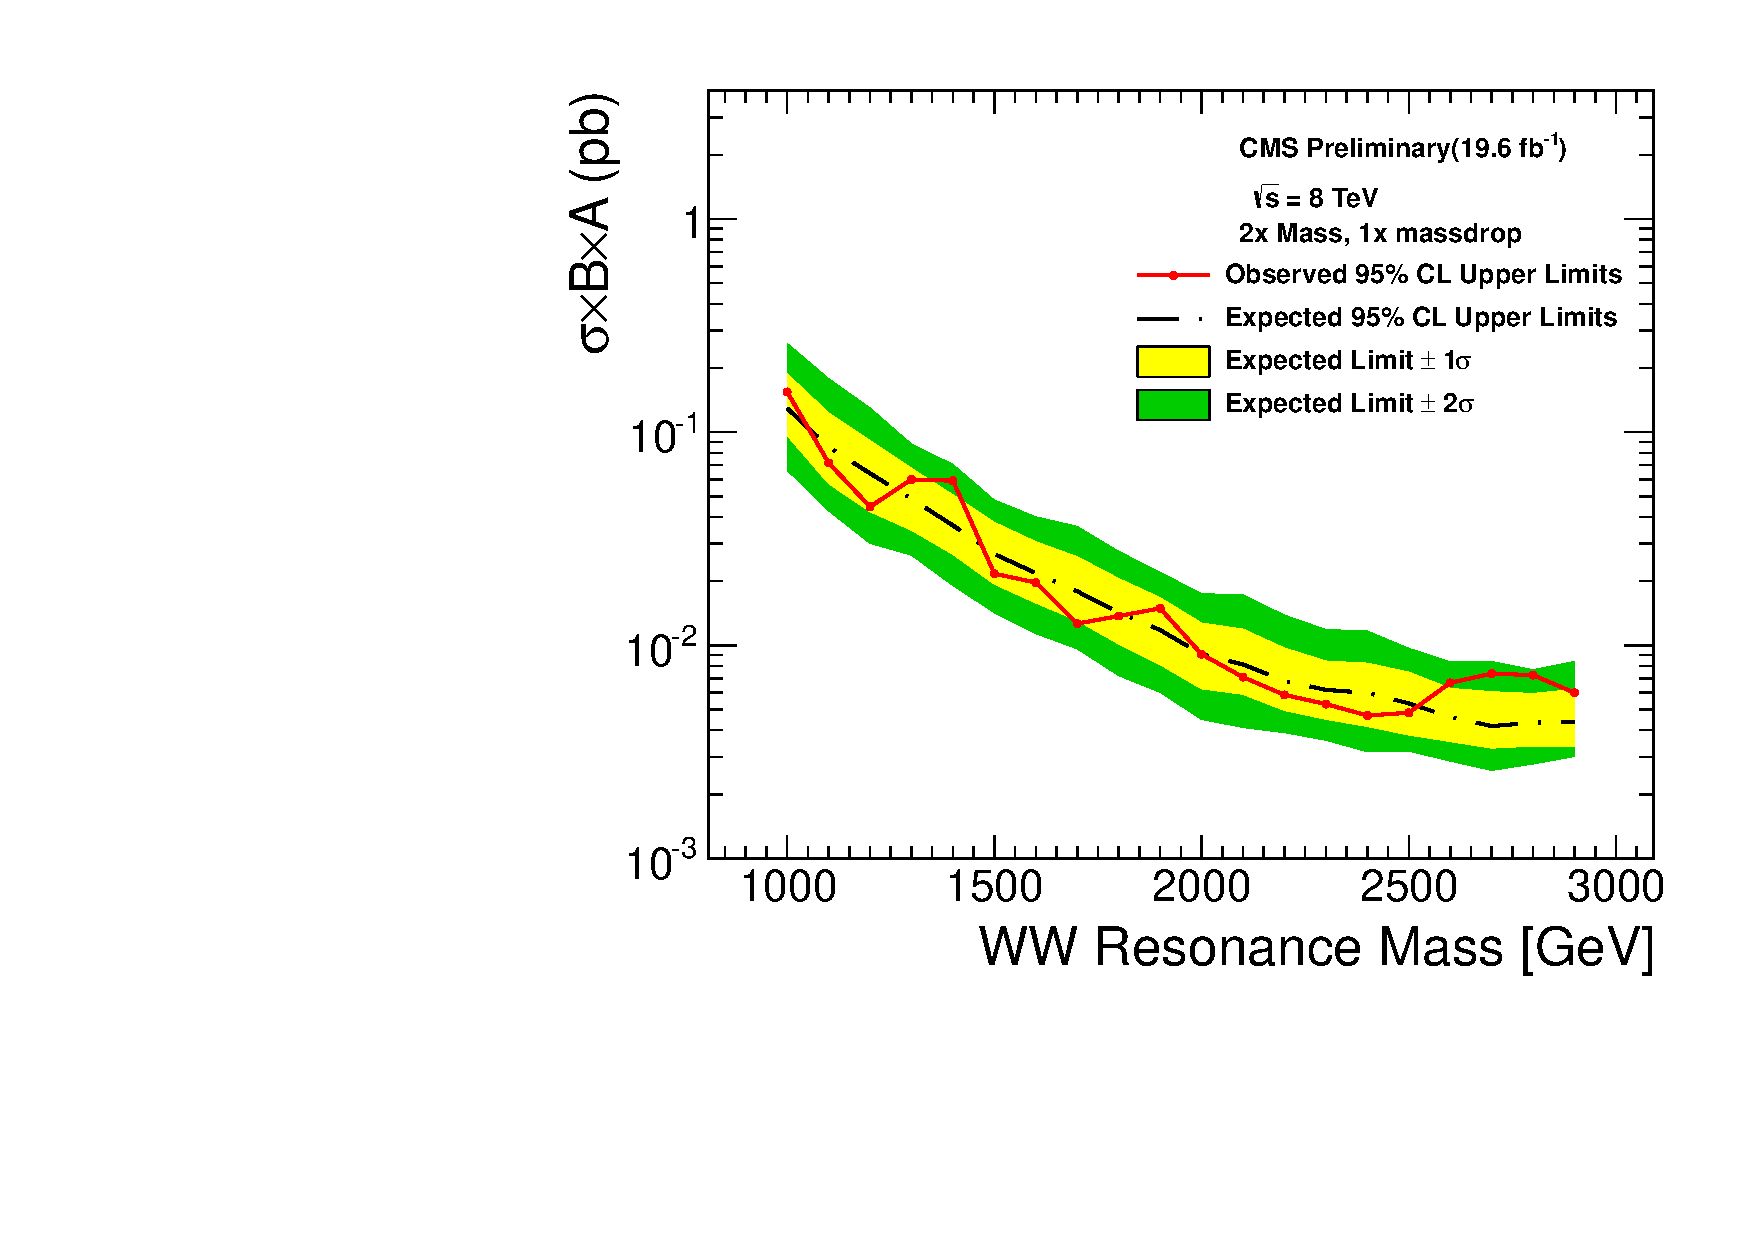
\includegraphics[width=0.48\textwidth,angle=0]{EXO-12-024/figs/VVCheck/RSGWWherwig_2xMass1xMassdrop_limit_obsexp.pdf}
%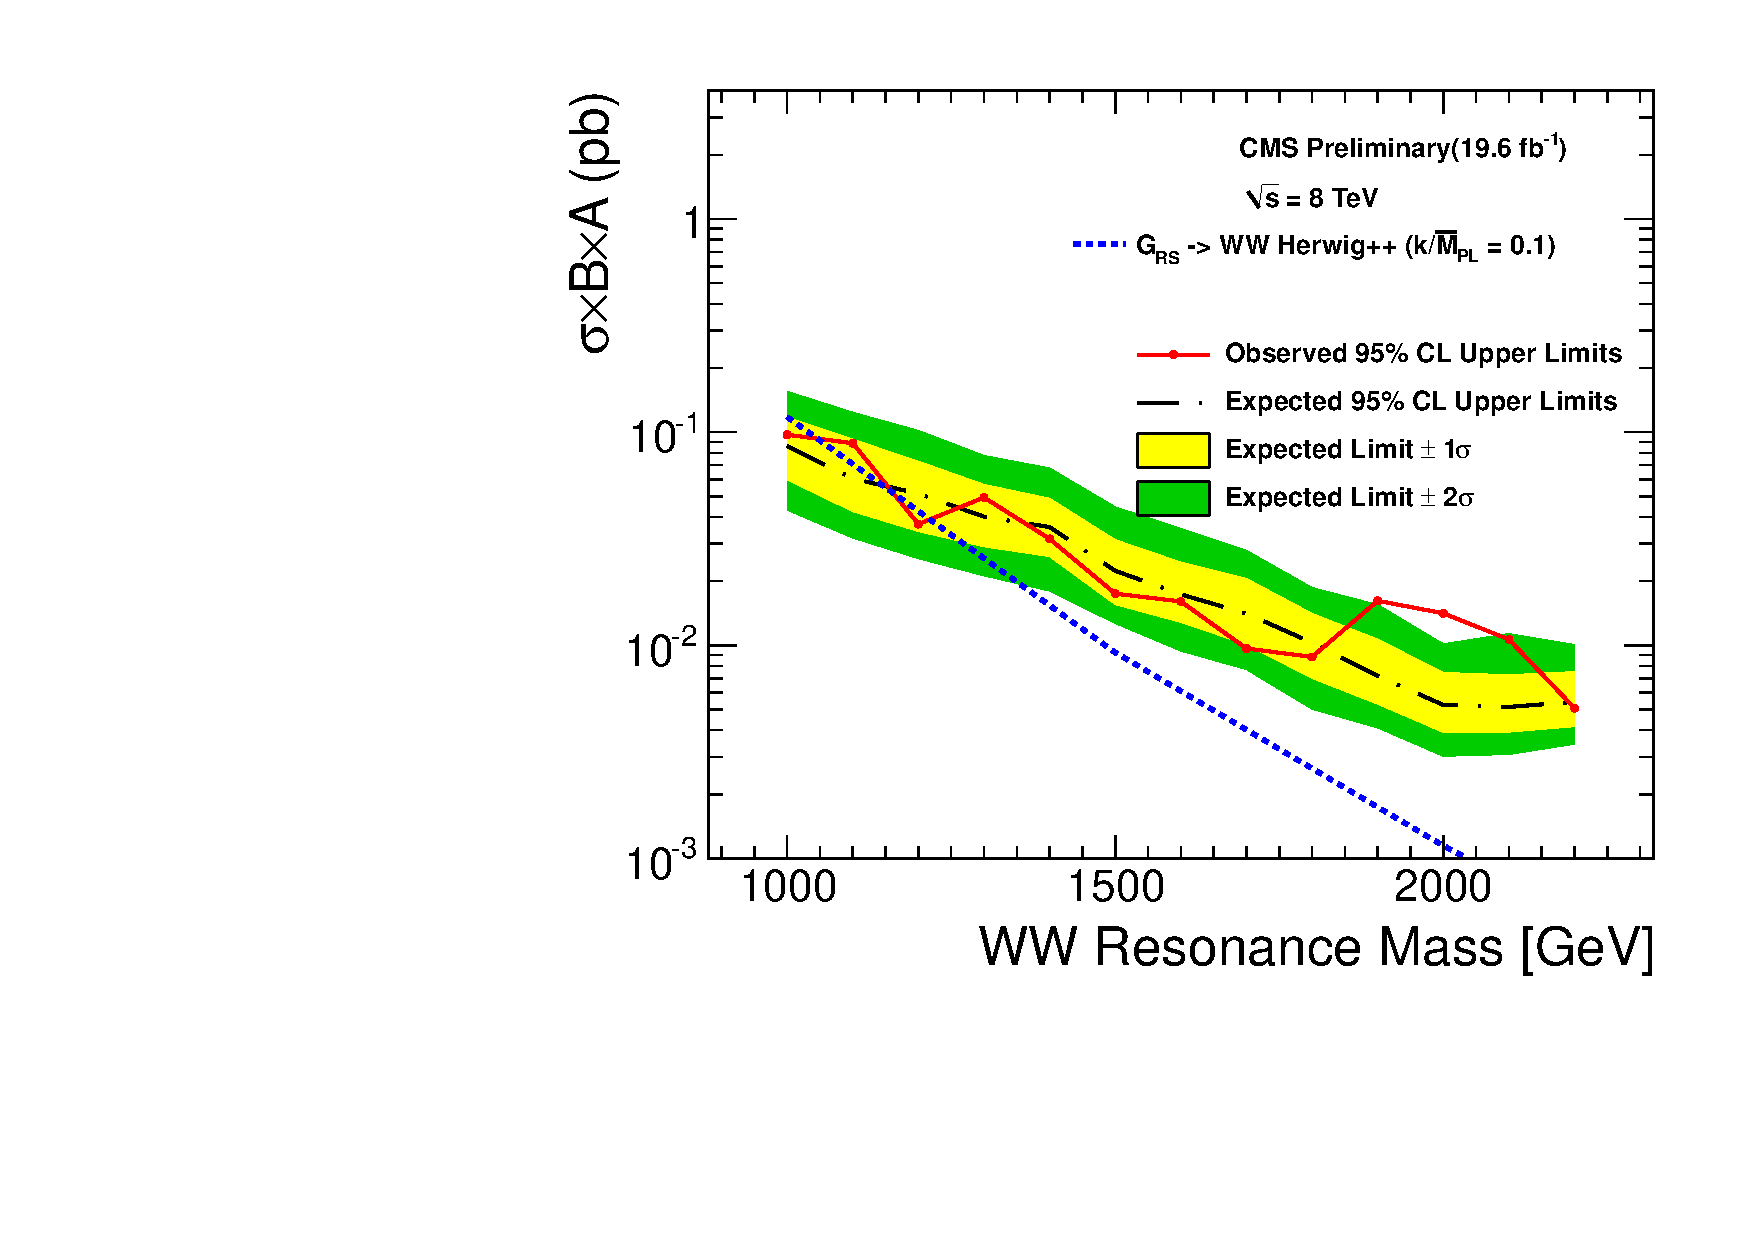
\includegraphics[width=0.48\textwidth,angle=0]{EXO-12-024/figs/VVCheck/RSGWWherwig_2Tag_limit_obsexp.pdf}
%\end{center}
%\caption{limits for categories e and f}
%\label{fig:eflimit}
%\end{figure}
%
%\begin{figure}[htb]
%\begin{center}
%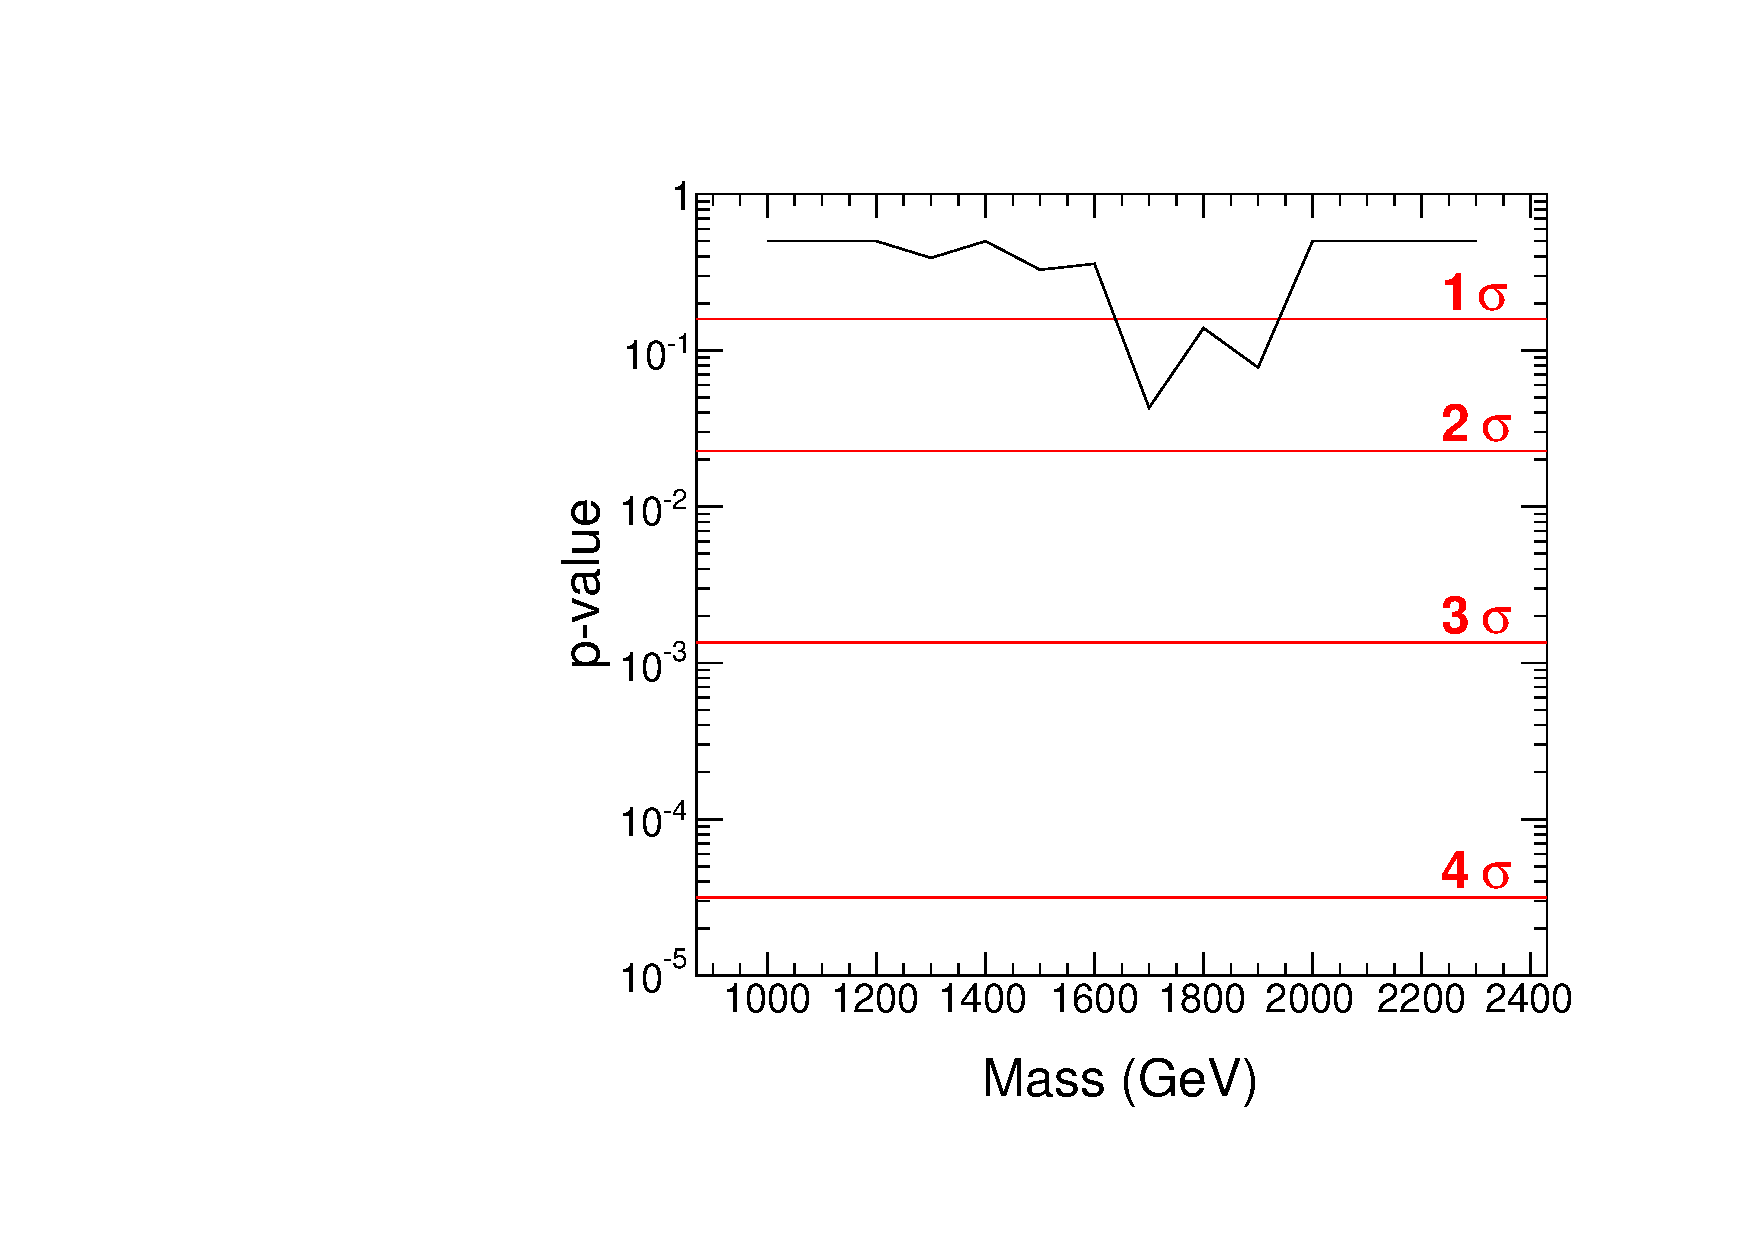
\includegraphics[width=0.48\textwidth,angle=0]{EXO-12-024/figs/appendix/pvalue_WW_channel5_m0.pdf}
%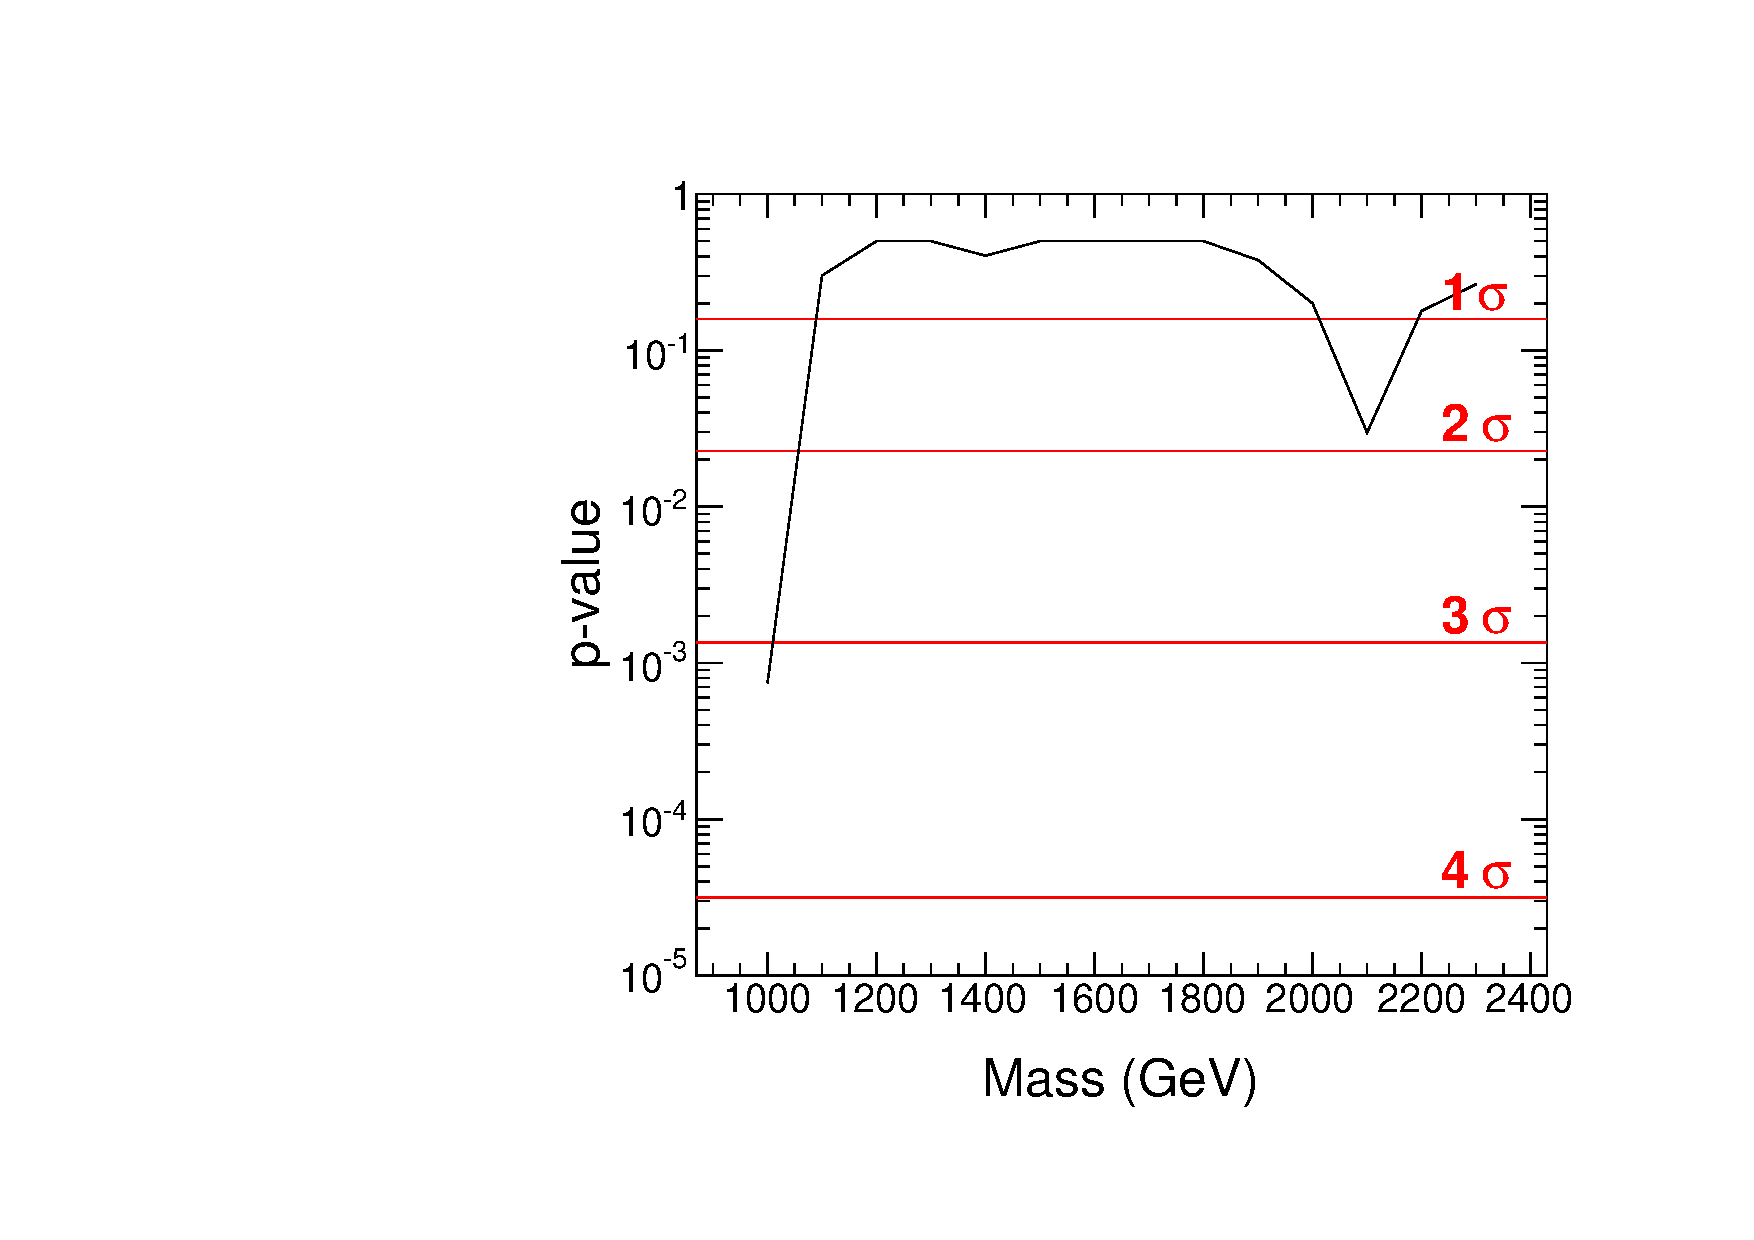
\includegraphics[width=0.48\textwidth,angle=0]{EXO-12-024/figs/appendix/pvalue_WW_channel3_m1mg0.pdf}
%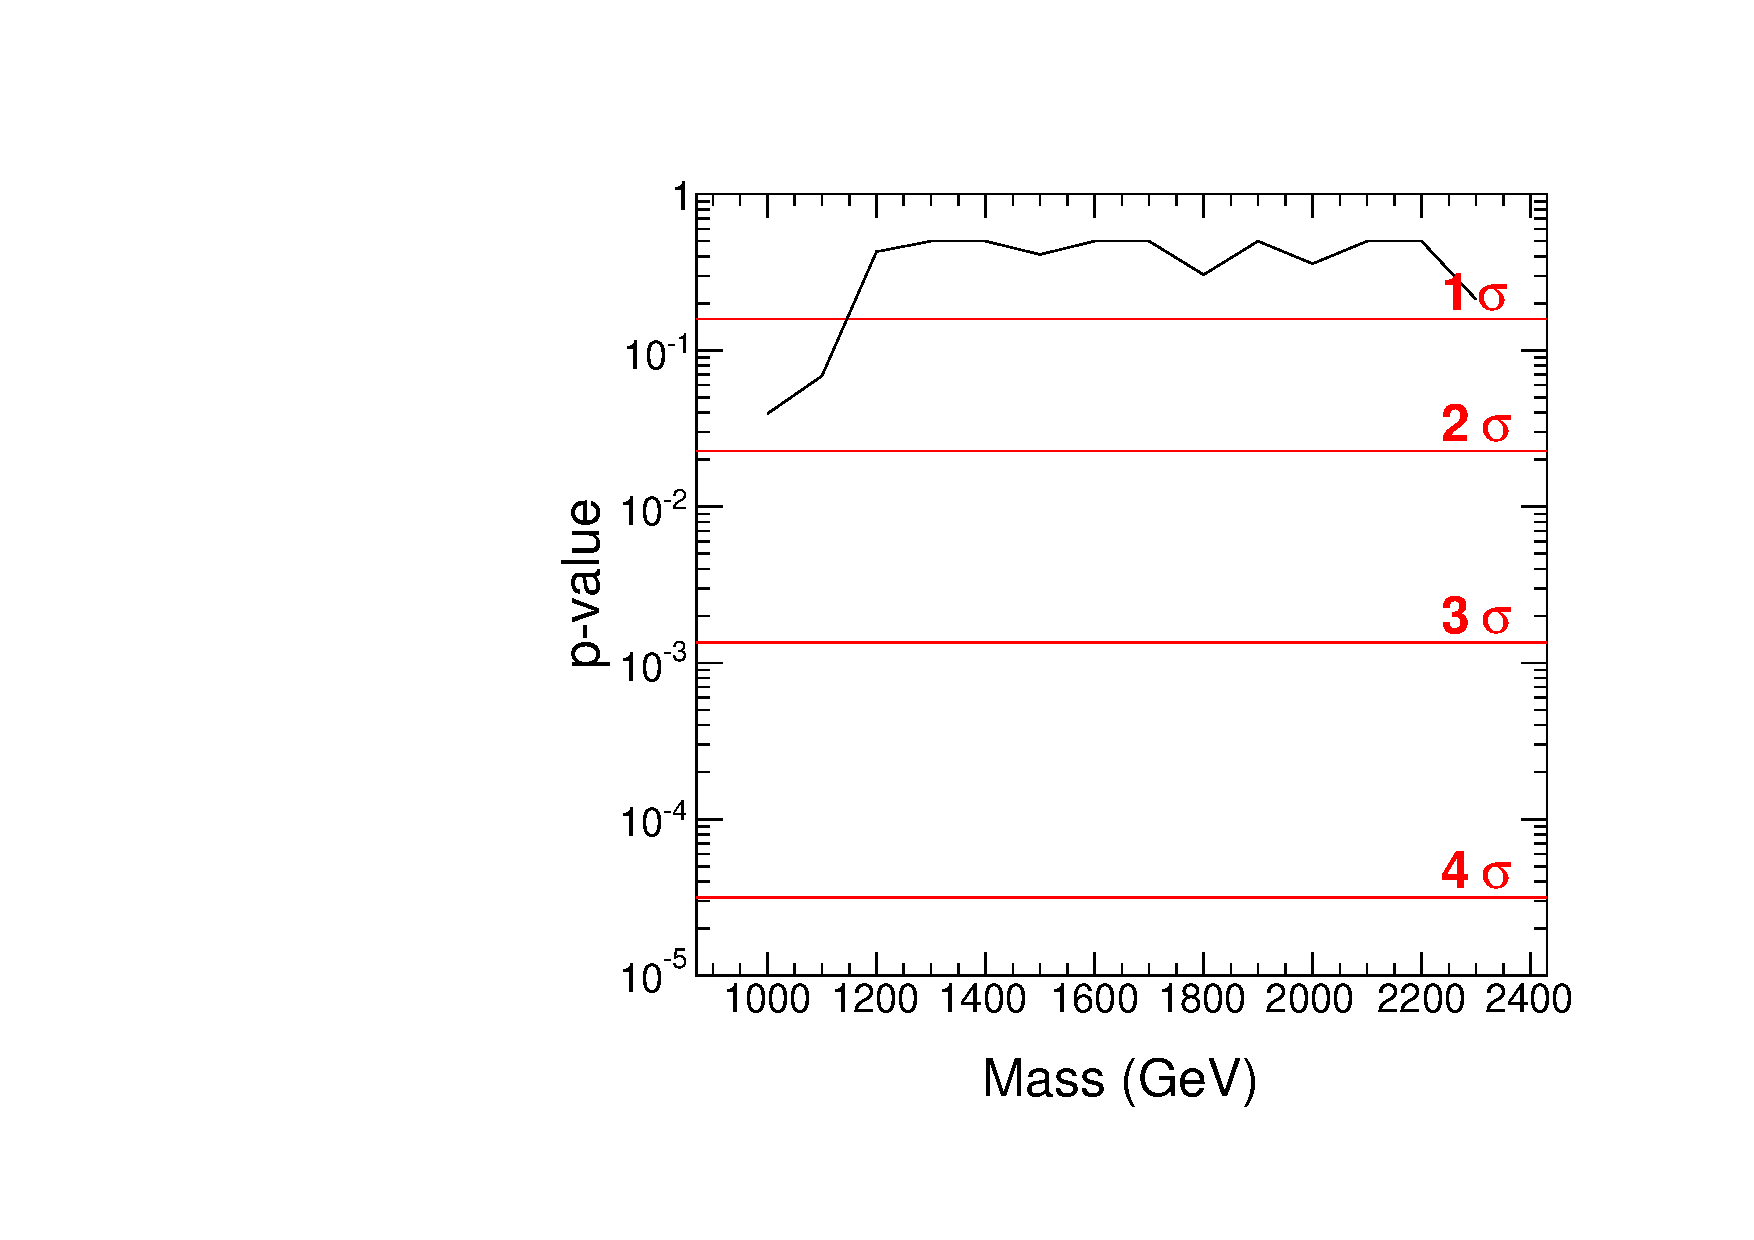
\includegraphics[width=0.48\textwidth,angle=0]{EXO-12-024/figs/appendix/pvalue_WW_channel4_m1mg1.pdf}
%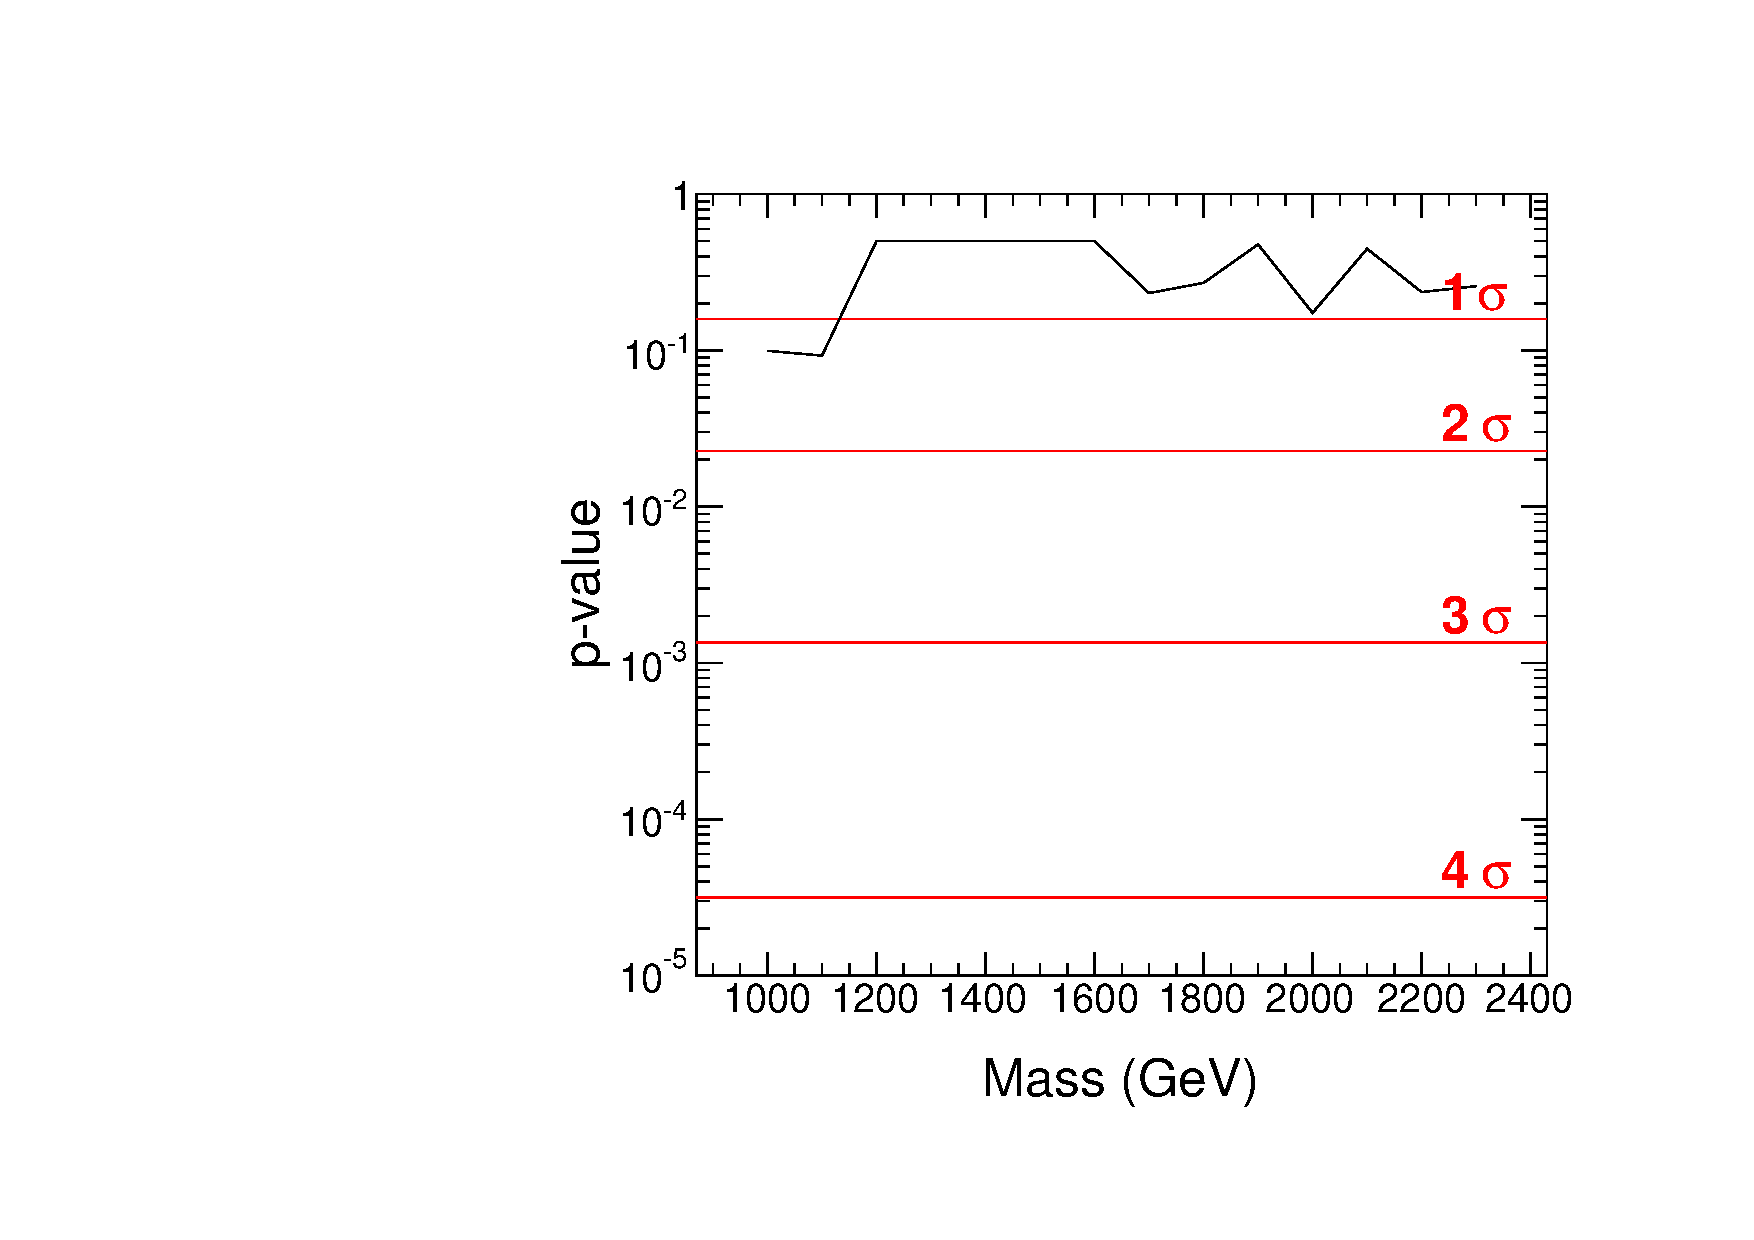
\includegraphics[width=0.48\textwidth,angle=0]{EXO-12-024/figs/appendix/pvalue_WW_channel0_m2mg0.pdf}
%\includegraphics[width=0.48\textwidth,angle=0]{EXO-12-024/figs/appendix/pvalue_WW_channel1_m2mg1.pdf}
%\includegraphics[width=0.48\textwidth,angle=0]{EXO-12-024/figs/appendix/pvalue_WW_channel2_m2mg2.pdf}
%\end{center}
%\caption{Local p-value in categories a, b, c, d, e, f as a function of the WW resonance mass.}
%\label{fig:app}
%\end{figure}
%
%\begin{figure}[htb]
%\begin{center}
%\includegraphics[width=0.48\textwidth,angle=0]{EXO-12-024/figs/appendix/pvalue_ZZ_channel5_m0.pdf}
%\includegraphics[width=0.48\textwidth,angle=0]{EXO-12-024/figs/appendix/pvalue_ZZ_channel3_m1mg0.pdf}
%\includegraphics[width=0.48\textwidth,angle=0]{EXO-12-024/figs/appendix/pvalue_ZZ_channel4_m1mg1.pdf}
%\includegraphics[width=0.48\textwidth,angle=0]{EXO-12-024/figs/appendix/pvalue_ZZ_channel0_m2mg0.pdf}
%\includegraphics[width=0.48\textwidth,angle=0]{EXO-12-024/figs/appendix/pvalue_ZZ_channel1_m2mg1.pdf}
%\includegraphics[width=0.48\textwidth,angle=0]{EXO-12-024/figs/appendix/pvalue_ZZ_channel2_m2mg2.pdf}
%\end{center}
%\caption{Local p-value in categories a, b, c, d, e, f as a function of the ZZ resonance mass.}
%\label{fig:app}
%\end{figure}

%\begin{figure}[htb]
%\begin{center}
%\includegraphics[width=0.48\textwidth,angle=0]{EXO-12-024/figs/appendix/brazilianFlag_acc_WW_m2mg2.pdf}
%\includegraphics[width=0.48\textwidth,angle=0]{EXO-12-024/figs/appendix/brazilianFlag_acc_WW_m2mg1.pdf}
%\includegraphics[width=0.48\textwidth,angle=0]{EXO-12-024/figs/appendix/brazilianFlag_acc_WW_m2mg0.pdf}
%\includegraphics[width=0.48\textwidth,angle=0]{EXO-12-024/figs/appendix/brazilianFlag_acc_WW_m1mg1.pdf}
%\includegraphics[width=0.48\textwidth,angle=0]{EXO-12-024/figs/appendix/brazilianFlag_acc_WW_m1mg0.pdf}
%\includegraphics[width=0.48\textwidth,angle=0]{EXO-12-024/figs/appendix/brazilianFlag_acc_WW_0m.pdf}
%\end{center}
%\caption{THESE FIGURES ARE NOT PROPERLY NORMALIZED}
%\label{fig:app}
%\end{figure}

%\clearpage
%\subsection{Jet mass and massDrop correlation}

%\begin{figure}[htb]
%\begin{center}
%\includegraphics[width=0.48\textwidth,angle=0]{EXO-12-024/figs/MassAndDrop/DataMassAndDrop0.pdf}
%\includegraphics[width=0.48\textwidth,angle=0]{EXO-12-024/figs/MassAndDrop/DataMassAndDrop1.pdf}
%\end{center}
%\caption{Data leading jet mass and massdrop correlation(left);data second leading jet mass and massdrop correlation(right). }
%\label{fig:data}
%\end{figure}

%\begin{figure}[htb]
%\begin{center}
%\includegraphics[width=0.48\textwidth,angle=0]{EXO-12-024/figs/MassAndDrop/QCDHerwigMassAndDrop0.pdf}
%\includegraphics[width=0.48\textwidth,angle=0]{EXO-12-024/figs/MassAndDrop/QCDHerwigMassAndDrop1.pdf}
%\end{center}
%\caption{QCD herwig leading jet mass and massdrop correlation(left);QCD herwig second leading jet mass and massdrop correlation(right). }
%\label{fig:QCDherwig}
%\end{figure}


%\begin{figure}[htb]
%\begin{center}
%\includegraphics[width=0.48\textwidth,angle=0]{EXO-12-024/figs/MassAndDrop/SignalHerwig1TeVMassAndDrop0.pdf}
%\includegraphics[width=0.48\textwidth,angle=0]{EXO-12-024/figs/MassAndDrop/SignalHerwig1TeVMassAndDrop1.pdf}
%\end{center}
%\caption{Signal 1 \TeVcc herwig leading jet mass and massdrop correlation(left);signal 1 \TeVcc herwig second leading jet mass and massdrop correlation(right). }
%\label{fig:signalherwig}
%\end{figure}

\clearpage

\section{Limit calculation cross check}

\begin{figure}[htb]
\begin{center}
\includegraphics[width=0.52\textwidth,angle=0]{EXO-12-024/figs/appendix/RSGWWherwig_2Tag_limit_obsexp.pdf}
\includegraphics[width=0.44\textwidth,angle=0]{EXO-12-024/figs/appendix/brazilianFlag_acc_WW_m2mg2.pdf}
\end{center}
\caption{Expected and observed limits on WW resonances in the 2-tag category.
Left: Bayesian type limits as explained in section. Right: Asymptotic CLs type limits.}
\label{fig:app}
\end{figure}
